\appendix

\section{Notation}
\label{app:notation}

This appendix summarizes our notation and lists the symbols used throughout
the paper, together with the section, equation, or algorithm where each is
defined.

\paragraph{Conventions.}
Lowercase italic letters denote scalars ($t$, $g_\ell$), bold lowercase
letters denote vectors ($\mathbf{x}$, $\mathbf{a}_{ij}$), uppercase italic
letters denote matrices ($W_{\mathrm{dec}}$, $D_i$), and sans-serif letters
denote tensors of rank three or more ($\mathsf{D}$, $\mathsf{P}$). A
subscripted object takes the font corresponding to its own rank: $p_{nij}$
is a scalar element of $\mathsf{P}$, $\mathbf{p}_{ni}$ is a vector slice,
and $D_i := \mathsf{D}_{i\cdot\cdot}$ is a matrix slice; where a lowercase
element could be confused with a reserved count, we enclose it in brackets,
as in $[\mathsf{K}]_{nij}$. Batching adds a leading dimension: a single
sample's assignments are $P \in \mathbb{R}^{h\times k}$, whereas a batch's
are $\mathsf{P} \in \mathbb{R}^{b\times h\times k}$. Vectors are column
vectors, so matrices act on the left ($W_{\mathrm{dec}}\mathbf{r}_\ell$,
with $W_{\mathrm{dec}} \in \mathbb{R}^{d\times e}$ mapping $\mathbb{R}^e$
to $\mathbb{R}^d$). Batches stack samples as rows
($X \in \mathbb{R}^{b\times d}$), so a batched matrix product carries a
transpose, $\hat{X} = R\,W_{\mathrm{dec}}^\top$, or is written as function
application, $\mathrm{dec}(R)$. Sets are written in calligraphic type
($\mathcal{S}_n$, $\mathcal{G}$). Named statistics, losses, and operators
are set in roman type ($\fvu$, $\mathrm{MSE}$, $\mathrm{KL}_m$,
$\mathrm{dec}$, $\mathrm{sg}$), while $H$ denotes entropy and $L$ denotes
the total loss; the discussion around Eq.~\eqref{eq:realized} follows
standard information-theoretic convention by writing random variables in
uppercase. A hat denotes a reconstruction ($\hat{\mathbf{x}}_\ell$), a
tilde denotes a noised quantity ($\tilde{\mathsf{F}}$,
$\tilde{\mathbf{f}}_i$), a bar denotes a mean ($\bar{\mathbf{p}}_i$,
$\bar\kappa$), and a prime on an index denotes a second index of the same
kind ($i'$, $j'$). We write $\odot$ for the elementwise product and
$\oplus$ for concatenation. Cosine similarity is written as the cosine of
the angle between two vectors,
$\cos\angle(\mathbf{a}, \mathbf{b}) :=
\langle\mathbf{a},\mathbf{b}\rangle / (\lVert\mathbf{a}\rVert\lVert\mathbf{b}\rVert)$,
so that $\cos$ takes a single argument; $\lvert\cos\angle\rvert$ alone
denotes its absolute value for the vector pair in context. The expectation
operator $\mathbb{E}$ averages over the index or distribution named in its
subscript: $\mathbb{E}_n$ over the samples in context (a batch in a
training statistic, or the scored rows in an evaluation), $\mathbb{E}_i$
over heads, $\mathbb{E}_{i \neq i'}$ over ordered pairs of distinct heads,
and $\mathbb{E}_{j \sim \bar{\mathbf{p}}_i}$ under a distribution. When
unsubscripted, $\mathbb{E}$ averages over the data. Similarly, $\Pr$
denotes an empirical fraction of samples, with $\Pr_n(\cdot)$ giving the
fraction on which the condition holds. Finally, $\mathbf{1}[\cdot]$ denotes
the indicator function, and $\mathrm{sd}$ and $\mathrm{var}$ denote the
standard deviation and variance, subscripted under the same convention as
$\mathbb{E}$.

\paragraph{Layers and states.}
Layers are indexed by position, $\ell = 0,\dots,l-1$, and states of the
residual stack are indexed by the number of layers applied, $0,\dots,l$, so
that layer $\ell$ takes state $\ell$ as input and produces state $\ell+1$.
Under this convention, $\mathbf{r}_0 = \mathbf{0}$ and
$\mathbf{y}_0 = \mathbf{x}$, the final reconstruction is
$\hat{\mathbf{x}}_l$, and the deep-supervision prefixes are
$\hat{\mathbf{x}}_1,\dots,\hat{\mathbf{x}}_l$. Because prose and tables
refer to layers by index (e.g., ``layer 0''), a table row for layer $\ell$
reports the prefix reconstruction through that layer,
$\hat{\mathbf{x}}_{\ell+1}$.

\paragraph{Indices and sizes.}
\begin{center}\small
\begin{tabular}{@{}llll@{}}
\toprule
index & ranges over & size & \\
\midrule
$n$, $n'$ & samples & $b$ & batch size \\
$\ell$, $\ell'$ & layers, $0,\dots,l-1$ & $l$ & layers \\
$i$, $i'$ & heads of a layer & $h$ & heads per layer \\
$j$, $j'$ & entries of a head & $k$ & entries per head \\
$q$ & coordinates & $d$, $e$ & input dimension, dictionary width \\
\midrule
& & $r$ & fiber rank \\
& & $d_{\mathrm{head}}$ & a head's slice of $e$ under concatenated heads \\
& & $k_{\mathrm{sel}}$ & entries kept by the \texttt{top}$k_{\mathrm{sel}}$ selection rule \\
& & $h'$ & heads kept, probed, or conjoined, out of $h$ \\
& & $n_{\mathrm{const}}$ & constant coordinates appended to a layer's input \\
& & $m$, $k_{\mathrm{SAE}}$ & SAE width, and active latents under $\topk$ \\
\bottomrule
\end{tabular}
\end{center}
Throughout the paper, $k$ without a subscript denotes the number of
Ontologizer entries per head.

\paragraph{Symbols.}
The table below lists all symbols grouped by the component of the paper
that introduces them.

\begingroup\small
\begin{longtable}{@{}>{\raggedright\arraybackslash}p{0.25\linewidth}%
>{\raggedright\arraybackslash}p{0.52\linewidth}%
>{\raggedright\arraybackslash}p{0.15\linewidth}@{}}
\toprule
symbol & meaning & defined \\
\midrule
\endfirsthead
\toprule
symbol & meaning & defined \\
\midrule
\endhead
\bottomrule
\endfoot
\bottomrule
\endlastfoot
\multicolumn{3}{@{}l}{\emph{The model}} \\[2pt]
$\mathbf{x}$, $X$; $\bar{\mathbf{x}}$ & an input ($d$) and a batch ($b\times d$); the data mean & Eqs.~\eqref{eq:mse}, \eqref{eq:fvu} \\
$\mathrm{enc}$ & input encoder (the identity map unless stated otherwise) & Alg.~\ref{alg:ontologizer} \\
$\mathbf{u}_\ell$, $\mathbf{u}$ & layer $\ell$'s normalized input shape, with the constant coordinate appended, passed to the classifier, router, and fibers ($\mathbf{u}$ within a layer) & Eq.~\eqref{eq:y_norm} \\
$\mathsf{W}$, $\mathsf{V}$ & the bilinear classifier's weight tensors & Eq.~\eqref{eq:bilinearblock} \\
$K$, $\mathsf{K}$ & classifier logits for one sample ($h\times k$) and for a batch & Eq.~\eqref{eq:bilinearblock} \\
$t$ & classifier temperature, $P = \mathrm{softmax}_k(K/t)$ & §\ref{sec:labels} \\
$P$, $\mathsf{P}$; $\mathbf{p}_{ni}$, $p_{nij}$ & assignments for one sample and a batch; head $i$'s distribution and entry $j$'s probability & §\ref{sec:labels} \\
$\bar{\mathbf{p}}_i$ & head $i$'s mean assignment (entry usage) over the data & Eq.~\eqref{eq:KL} \\
$p_{\mathrm{drop}}$ & winner-dropout probability & §\ref{sec:bilinear} \\
$\mathsf{D}$, $D_i$ & dictionary tensor ($h\times k\times e$) and head $i$'s slice ($k\times e$) & Eq.~\eqref{eq:dictblock} \\
$\mathbf{a}_{ij}$ & an atom: $\lvert\mathsf{D}_{ij\cdot}\rvert$, or $\mathsf{D}_{ij\cdot}$ when signed & Eq.~\eqref{eq:dictblock} \\
$G_i$ & head $i$'s dictionary Gram matrix & Eq.~\eqref{eq:cossim_b} \\
$\mathbf{f}_i$; $F$, $\mathsf{F}$ & head $i$'s output ($e$); stacked over heads, and over heads and samples & Eq.~\eqref{eq:dictblock} \\
$\mathbf{f}'_\ell$, $F'$ & layer $\ell$'s pooled output for one sample and for a batch & Eq.~\eqref{eq:pool} \\
$\boldsymbol{\gamma}$, $\gamma_i$, $\Gamma$ & router scales across heads, for head $i$, and for a batch & Eq.~\eqref{eq:fiber} \\
$U_{ij}$, $\mathbf{c}_i$; $C$, $\mathsf{C}$ & fiber basis ($e\times r$) and coordinates; stacked over heads and over a batch & Eq.~\eqref{eq:fiber} \\
$\mathsf{A}$, $A_i$; $\beta$, $\rho$ & fiber readout tensor and head $i$'s slice; coordinate bound and norm cap & §\ref{sec:router-fiber} \\
$g_\ell$, $g_n$ & scalar gain: input norm at layer $\ell$ or for sample $n$ & Eq.~\eqref{eq:accum} \\
$\mathbf{r}_\ell$, $R$ & residual accumulator after $\ell$ layers, for one sample and batched & Eq.~\eqref{eq:accum} \\
$W_{\mathrm{dec}}$, $\mathrm{dec}$ & linear decoder shared across all layers & Eq.~\eqref{eq:dec} \\
$\hat{\mathbf{x}}_\ell$, $\hat{X}$ & reconstruction after $\ell$ layers; final batched reconstruction & Eq.~\eqref{eq:dec} \\
$\mathbf{y}_\ell$ & residual after $\ell$ layers (the input to layer $\ell$) & Eq.~\eqref{eq:L2} \\
$\mathrm{sg}[\cdot]$ & stop-gradient operator & Eq.~\eqref{eq:L2} \\
$W_{\mathrm{flat}}$ & code-to-output map of a model's flattened code, $\hat{\mathbf{x}} = W_{\mathrm{flat}}\mathbf{p}_{\mathrm{flat}}$, whose columns are the entries' decode directions & §\ref{app:protocols} \\
\addlinespace
\multicolumn{3}{@{}l}{\emph{Noise, statistics, and loss}} \\[2pt]
$\varepsilon$; $\varepsilon_K$, $\varepsilon_F$ & standard normal draw; logit and feature noise terms & §\ref{sec:noise} \\
$\sigma_X$, $\sigma_K$, $\sigma_F$ & noise scales for inputs, logits, and features & §\ref{sec:noise} \\
$\tilde{\mathsf{F}}$, $\tilde{\mathbf{f}}_i$ & noised per-head outputs & Eq.~\eqref{eq:L1} \\
$\epsilon$ & floating-point epsilon of the working dtype & Eq.~\eqref{eq:y_norm} \\
$\tau_{\mathrm{rev}}$ & dead-entry revival threshold & Alg.~\ref{alg:dictblock} \\
$\mathrm{entropy}_k$, $H$ & entropy of a head's assignment in bits, and its mean over samples and heads & Eq.~\eqref{eq:entropy} \\
$\mathrm{cossim}_b$ & between-sample similarity of per-head outputs & Eq.~\eqref{eq:cossim_b} \\
$\mathrm{KL}_m$ & divergence of each head's batch-mean assignment from uniform, averaged over heads & Eq.~\eqref{eq:KL} \\
$\kappa_i$, $\bar\kappa$ & mean cosine between head $i$'s atoms, and its mean over heads (row collinearity) & Eq.~\eqref{eq:stats}; §\ref{sec:rowcos} \\
$\boldsymbol{\pi}_i$, $\omega$ & head $i$'s usage-weighted coordinate profile; between-head support overlap & Eq.~\eqref{eq:support} \\
$\mathrm{L1}$, $\mathrm{L1}_K$, $\mathrm{L1}_S$ & L1 penalties on features, classifier gates, and router scales & Eqs.~\eqref{eq:L1}, \eqref{eq:stats} \\
$\mathrm{KL}_{\mathrm{pwak}}$, $\mathrm{L2}_{\mathrm{pwak}}$ & partition-consensus statistics & Eq.~\eqref{eq:stats} \\
$\boldsymbol{\psi}_\ell$ & layer $\ell$'s statistics row & Eq.~\eqref{eq:stats} \\
$\mathbf{w}$ & per-dimension MSE weights: inverse variance, normalized to mean one & Eq.~\eqref{eq:mse} \\
$\mathbf{s}$; $s_g$, $s_\omega$, $s_{\mathrm{L1}}$, \dots & loss weights: the vector paired with $\boldsymbol{\psi}_\ell$, and individual weights & Eq.~\eqref{eq:loss_total} \\
$\mathrm{MSE}$, $L$ & whitened reconstruction error; total training loss & Eqs.~\eqref{eq:mse}, \eqref{eq:loss_total} \\
\addlinespace
\multicolumn{3}{@{}l}{\emph{Evaluation and baselines}} \\[2pt]
$\fvu$ & whitened fraction of variance unexplained & Eq.~\eqref{eq:fvu} \\
$\nu$, $\mathcal{S}_\nu$; $\mathbf{o}$ & deviations retained per head and their support set; mean-assignment origin & Eq.~\eqref{eq:topdev} \\
$\mathrm{FVU}_{w,\mathrm{G}}$, $n_{\mathrm{bits}}$; $\lambda_j$, $\theta$ & Gaussian rate--distortion reference and bit budget; covariance eigenvalues and reverse water-filling level & Eq.~\eqref{eq:ratefloor} \\
$H_{\mathrm{real}}$ & realized bits: summed per-head entropy of entry usage & Eq.~\eqref{eq:realized} \\
$\Delta$, $\Delta_j$; $H_{\mathrm{op}}$ & quantizer step size, shared and for coefficient $j$; operational rate in bits per sample & Eq.~\eqref{eq:quantrate} \\
$\mathcal{G}$; $\mathrm{exh}$, $\mathrm{exc}$ & a head or latent group; its exhaustiveness and exclusivity & Eq.~\eqref{eq:exhaust} \\
$\kappa(\mathcal{G})$, $\zeta_{\cos}$; $\mathbf{v}_j$ & within-group mean decode-direction cosine and its standardized score; a decode direction & Eq.~\eqref{eq:zcos} \\
$(\cdot)^{(1)}$, $(\cdot)^{(2)}$ & the two models in a pairwise comparison & Eq.~\eqref{eq:headmatch} \\
$\mathbf{q}^{(1)}_i$; $[M^{\mathrm{part}}]_{ii'}$, $[M^{\mathrm{contr}}]_{ii'}$ & head $i$'s entry selections across rows; head-matching similarity matrices & Eq.~\eqref{eq:headmatch} \\
$\boldsymbol{\phi}_{ni}$, $\mathrm{size}_i$ & head $i$'s output contribution on sample $n$; its share of whitened variance & Eqs.~\eqref{eq:headmatch}, \eqref{eq:headsize} \\
$\mathbf{a}^{\mathrm{dec}}_{ij}$, $\bar{\mathbf{a}}^{\mathrm{dec}}_i$ & a decoded atom; head $i$'s usage-weighted mean decoded atom & Eq.~\eqref{eq:headsize} \\
$\mathrm{recovered}$ & fraction of next-token or decoder loss recovered & Eq.~\eqref{eq:lossrec} \\
$\eta^2$; $\mathcal{C}$, $n_{\mathrm{rows}}$ & fraction of variance explained by a partition; its cells and number of scored rows & Eq.~\eqref{eq:eta} \\
$k_{\mathrm{probe}}$ & sparse-probing budget & §\ref{app:protocols} \\
$\mathbf{z}^\star_n$, $\mathcal{S}_n$; $W$, $\mathbf{b}$ & refitted coefficients on a frozen support; a linear code's decode directions (columns of $W$) and offset & Eq.~\eqref{eq:refit} \\
$\mu_{ni}$; $j_1$, $j_2$; $J_i$; $\alpha$ & a head's logit margin between its top two entries; Jacobian of head $i$'s logits; step strength & Eq.~\eqref{eq:flip} \\
$j^\star$, $\mathrm{dir}$, $\boldsymbol{\xi}_n$ & steering target entry, steering direction, and random control vector & Alg.~\ref{alg:steerembed} \\
$\mathrm{assign}$ & abstraction map from an input to its code & §\ref{sec:formal} \\
$\mathbf{z}$, $z_{nj}$ & SAE latent activations & Eq.~\eqref{eq:exhaust} \\
$W_{\mathrm{enc}}$, $\mathbf{b}_{\mathrm{enc}}$; $W_{\mathrm{dec}}$, $\mathbf{b}_{\mathrm{dec}}$ & SAE encoder weights and bias; SAE decoder (whose columns are decoder directions) and pre-subtracted decoder bias & §\ref{sec:models} \\
$\mathrm{L0}$, $s_{\mathrm{L1}}$, \texttt{aux\_k} & active SAE latents per sample; L1 penalty weight; dead-latent revival count & §\ref{sec:models}; Table~\ref{tab:cfg-sae} \\
\end{longtable}
\endgroup

\section{Supplementary methods}
\label{app:methods}

\subsection{Data and objective}
\label{app:data}

\paragraph{Embedding space and data.}
All main SONAR models are trained on a fixed cache of 4{,}000{,}000
unit-norm SONAR sentence embeddings ($d{=}1024$) computed from an
interleaved 86-language mC4 sample, paired with a ground-truth language
label sidecar. Because the stream order is deterministic, raw source text
is recoverable by row index and verified per row against the language
sidecar. Only six of the 86 configurations (English twice, French, Spanish,
German, and Chinese) were encoded under their native SONAR source-language
tags; the remaining 80 configurations (93\% of rows) were encoded under the
English tag, which specifies the source language to the SONAR encoder.
Re-encoding 400 rows per language under their intended native tags
(\texttt{experiments/\allowbreak lang-tags/\allowbreak retag.py}) shifts the
affected rows by $\fvu = 0.305$, roughly twice the hard code's
reconstruction error, with nearly all of the shift specific to individual
rows rather than a per-language offset. Ground-truth language accounts for
6.7\% of embedding variance under the English tag vs.\ 7.4\% under the
native tags, and reconstruction error on the re-tagged embeddings increases
by 4--12\% across both the hard-code Ontologizer and the SAEs. Throughout
the main SONAR experiments, ``SONAR embeddings'' refers to embeddings
computed under these cached tags, and the language-localization analyses
inherit that convention (Appendix~\ref{sec:langlocal}). The embedding
distribution lies on the unit sphere without being centered:
$\lVert\bar{\mathbf{x}}\rVert = 0.564$, forming a spherical cap in which a
single shared direction accounts for $0.318$ of every sample's squared
norm. It is high-dimensional yet anisotropic, with an effective dimension
of 108 out of 1024 (participation ratio 268 on the whitened evaluation
tail), 943 principal components required to explain 99\% of variance, and a
mean pairwise cosine of $0.31$. Sections~\ref{sec:gpt2}
and~\ref{sec:seeds} additionally evaluate residual-stream activations of
GPT-2 small~\cite{radford2019} leaving block 8 of 12
(\texttt{blocks.8.resid\_post}; $d{=}768$, harvested by
\texttt{encode\_acts.py}), a substrate where sparse dictionary learning is
well established~\cite{gao2024}. Section~\ref{sec:gpt2hard} uses a separate
GPT-2 configuration from the \texttt{headline} branch (the unwhitened
residual stream entering block 8 on FineWeb, also evaluated by GPT-2
next-token loss recovered), whose results are compared only within that
section.

\paragraph{Evaluation.}
All models minimize the whitened MSE of Eq.~\eqref{eq:mse}. We report
$\fvu$, defined as whitened MSE divided by the whitened variance around a
constant mean predictor,
\begin{equation}
	\fvu := \frac{\sum_{n} \sum_{q} w_q \,(\hat{x}_{n,q} - x_{n,q})^2}
	              {\sum_{n} \sum_{q} w_q \,(x_{n,q} - \bar{x}_q)^2},
	\qquad \bar{\mathbf{x}} := \mathbb{E}_n[\mathbf{x}_n],
	\label{eq:fvu}
\end{equation}
where $\mathbf{w}$ is the per-dimension inverse variance normalized to mean
one, evaluated on the final 32{,}768 rows of the cache. This evaluation
tail is held out from training for all SAEs and all straight-through arms.
Because the softmax Ontologizers (\texttt{resid\_nc} and the selection
sweep) predate the holdout split and were trained on the full cache, we
encoded the next 131{,}072 mC4 stream rows following the training corpus
under the identical pipeline (\texttt{encode\_fresh.py}), yielding an
out-of-sample set that no model observed during training. On these fresh
rows, every \texttt{pareto.py} operating point of \texttt{resid\_nc}, the
selection sweep's softmax run, the straight-through stack, and the SAEs
shifts by at most 0.3\% (one near-exact SAE at $\fvu = 10^{-4}$ shifts by
0.9\%), and every operational rate in Appendix~\ref{sec:quantrate} shifts
by at most 0.0004 in $\fvu$, confirming that the softmax models' tail
scores are not inflated by training overlap. Where feature activations are
required, Ontologizer features are the flattened per-head assignment
probabilities $P \in \Delta^{k}{}^{\,l\cdot h}$ evaluated at the run's
final temperature (entry $j$ of head $i$ in layer $\ell$ corresponds to
feature $(\ell h + i)k + j$, with firing threshold $2/k$), and SAE features
are latent activations (with firing threshold $0$, except that runs with
softmax heads use the above-uniform threshold $2/(m/h)$ for $h$ heads to
match the entry convention). Evaluating a softmax checkpoint at the default
temperature $1.0$ rather than its annealed temperature $0.03$ yields
$\fvu \approx 0.91$ even for a healthy model, making it indistinguishable
from a collapsed run; every reported score therefore uses each run's final
training temperature.

\paragraph{Coordinate~837 and the sentence-split cache (\texttt{mc4\_sent16}).}
Because SONAR's encoder applies a final LayerNorm prior to mean pooling,
every unnormalized embedding $\mathbf{x}^{\mathrm{raw}}$ lies in the affine
hyperplane $\sum_{q=1}^{d} (x^{\mathrm{raw}}_q - \beta_q)/\gamma_q = 0$.
In SONAR's pretrained weights, $\gamma_{837} = 0.00492$ is five times
smaller than the next smallest scale and $\beta_{837} = -0.340$ is thirty
times larger than typical, so coordinate~837 carries $97\%$ of the
hyperplane normal's squared length and is determined by the remaining
1{,}023 coordinates to a root-mean-square error of $1.9\times10^{-9}$
($1.2\times10^{-4}$ in float16 storage). On the L2-normalized cache
\texttt{mc4\_4M}, dividing by $\lVert\mathbf{x}^{\mathrm{raw}}\rVert$ turns
that fixed coordinate into an almost exact proxy for
$1/\lVert\mathbf{x}^{\mathrm{raw}}\rVert$ (Pearson correlation $0.996$ with
$\beta_{837}/\lVert\mathbf{x}^{\mathrm{raw}}\rVert$). Although it retains
the smallest variance and therefore receives the largest inverse-variance
weight ($w_{837} = 27.25$, or $2.66\%$ of total weight, with the top ten
coordinates accounting for $5.1\%$), $1/\lVert\mathbf{x}^{\mathrm{raw}}\rVert$
varies smoothly over the sphere. Consequently, every model reconstructs
coordinate~837 to $\mathrm{FVU}_{837} \le 0.088$, lower than its mean
coordinate error and accounting for at most $0.41\%$ of whitened error in
any sparse model (\texttt{coordfvu.py}); zeroing $w_{837}$ at evaluation
changes $\fvu$ by at most $+0.0043$ and leaves all model rankings unchanged.
A companion sentence-split cache, \texttt{mc4\_sent16}
(\texttt{experiments/\allowbreak sentence-split/}), segments the first
4{,}000{,}000 mC4 documents with SaT (\texttt{sat-3l-sm}, capped at 200
characters; the three-layer model slightly outperforms the twelve-layer
model on round-trip SONAR chrF2, $0.593$ vs.\ $0.583$, by avoiding
under-segmented long spans). It encodes up to 16 consecutive segments per
document ($44{,}104{,}959$ rows from $3{,}974{,}496$ documents: $59.1\%$
full sentences, $21.6\%$ newline-split lines, and $19.4\%$ length-capped
pieces) under each row's native fastText language tag (83 of 86 languages
mapped to their own NLLB tag), storing unnormalized float16 embeddings
alongside document-boundary and segment-kind sidecars. Without L2
normalization, coordinate~837 is nearly constant and receives
$w_{837} = 837$, or $81.8\%$ of the total inverse-variance weight. In
paired 369.5k-step training runs on a 4M-row slice with and without
$w_{837}$ (\texttt{ste\_h76\_sent16\_w837} vs.\ \texttt{\_no837}, alongside
matching \texttt{k32} SAEs), retaining $w_{837}$ leaves 265 SAE latents
dead ($16\times$ as many as in the masked run), whereas the SAE's decoder
bias absorbs the constant offset so that coordinate~837 contributes only
$0.03\%$ of its error compared to $2.0$--$3.4\%$ for the bias-free
Ontologizer. Masking $w_{837}$ resolves this pathology---improving $\fvu$
on the remaining 1{,}023 coordinates from $0.1489$ to $0.1462$ for the
Ontologizer and from $0.4596$ to $0.4538$ for the SAE---and reconstructing
coordinate~837 analytically from the LayerNorm hyperplane prior to M2M100
decoding recovers the $0.03$ chrF2 lost when it is left unconstrained.

\subsection{Models and baselines}
\label{sec:models}

Full configurations for all models are tabulated in
Appendix~\ref{app:configs}.

\paragraph{Softmax Ontologizers.}
The reference Ontologizer (\texttt{resid\_nc}) instantiates the
architecture of Section~\ref{sec:arch} with softmax selection across
$l{=}5$ residual layers of $h{=}32$ heads and $k{=}32$ entries per head.
Layers 0--3 trained cleanly (reducing prefix $\fvu$ from $0.129$ to
$0.0051$), whereas layer 4 froze 22 of 32 heads late in temperature
annealing and slightly degrades final reconstruction
(Section~\ref{sec:lastlayer}). A subsequent \emph{selection sweep} holds
this architecture fixed and varies only the \texttt{DictBlock} selection
rule (\texttt{top1}, \texttt{top2}, \texttt{top4}, \texttt{top8},
\texttt{top16}, and \texttt{softmax}), training each variant both with and
without a raised batch-mean uniformity weight $s_{\mathrm{KL}_m}$
(\texttt{\_shm}).

\paragraph{The straight-through arm.}
The straight-through trainer (\texttt{train\_ste.py}) imports the
\texttt{sonar.py} configuration and overrides \texttt{select="ste"},
selecting the one-hot argmax in the forward pass while using
$\mathrm{softmax}(K/t)$ as a surrogate gradient in the backward pass. Its
architecture, calibration, and initialization are detailed alongside its
results in Section~\ref{sec:ste}.

\paragraph{SAEs.}
Our SAE baselines follow the architecture of Gao et al.~\cite{gao2024},
computing pre-activations
$\mathrm{relu}(W_{\mathrm{enc}}(\mathbf{x}-\mathbf{b}_{\mathrm{dec}})+\mathbf{b}_{\mathrm{enc}})$
with $\topk$ selection of $k_{\mathrm{SAE}}$ active latents and
reconstructions $\hat{\mathbf{x}} = W_{\mathrm{dec}}\mathbf{z} + \mathbf{b}_{\mathrm{dec}}$.
Decoder directions (the columns of $W_{\mathrm{dec}}$) are renormalized to
unit norm after every step, the linear encoder is initialized to the
decoder's transpose, and dead latents are revived via \texttt{aux\_k} (512
dead latents weighted by $1/32$, with a latent marked dead after 1000 steps
without firing); all models are trained to convergence. Departing from the
recipe of Gao et al.~\cite{gao2024}, our $\topk$ pre-activation retains the
encoder bias $\mathbf{b}_{\mathrm{enc}}$ (which their $\topk$ encoder
omits), $\mathbf{b}_{\mathrm{dec}}$ is initialized to the data mean rather
than the geometric median, the reconstruction objective is whitened, Adam
runs with its default $\epsilon$ without weight averaging or
decoder-gradient projection, and training makes multiple passes over a
fixed embedding cache. ReLU+L1 SAEs replace $\topk$ selection with an L1
sparsity penalty and periodic neuron resampling.

\paragraph{The structural-ablation ladder.}
To attribute empirical differences to individual architectural choices
rather than to complete architectures, we train a ladder of SAE variants at
$m{=}5120$ on the same data and objective, each introducing a single
Ontologizer-style constraint:

\begin{center}
\begin{tabular}{@{}llll@{}}
\toprule
rung & run & added structure & analogue \\
\midrule
1  & \texttt{k32} & none ($\topk$, $k_{\mathrm{SAE}}{=}32$) & baseline \\
2a & \texttt{g160top1} & 160 heads, hard winner per head & hard heads, router \\
2b & \texttt{g160softmax} & 160 heads, softmax per head & heads (soft) \\
3  & \texttt{k32\_p5} & 5 nested prefix losses (matryoshka) & deepsup layers \\
--- & \texttt{k32\_bl} & bilinear encoder, $[\mathbf{x}{-}\mathbf{b}_{\mathrm{dec}};1]$ factors & bilinear classifier \\
\bottomrule
\end{tabular}
\end{center}

Rungs 2a and 2b partition the $m{=}5120$ latents into 160 heads of 32
entries, and we treat them as simplified Ontologizer variants rather than
external baselines. Per-head competition over a shared decoder reduces to a
single layer of linear classifiers selecting dictionary entries, omitting
the bilinear classifier, the residual stack, and the non-negative
dictionary. Specifically, \texttt{g160softmax} is a one-layer softmax
Ontologizer whose per-head coefficients sum to one, leaving each head
without an independent magnitude. Conversely, \texttt{g160top1} is a
one-layer hard-code Ontologizer with a scalar router fused into its
classifier: each head selects one entry by argmax, and the ReLU of the
winning logit scales that entry's unit-norm atom. This winning activation
plays the role of the per-head router scale
(Section~\ref{sec:router-fiber}), computed directly by the classifier
rather than by a separate projection, so the code's 160 continuous
coefficients act as router scales alongside its 800 index bits. Fusing the
router also trains hard selection without a straight-through estimator,
since the winning logit receives reconstruction gradients through its
scale while non-winning logits receive zero gradient. Equivalently, this
model is an SAE with a rectified local winner-take-all
activation~\cite{srivastava2013} applied within each head. From a vector
quantization perspective, both rungs take the form of a single additive
quantizer comprising 160 codebooks of 32 atoms that each span the output
space~\cite{babenko2014}: \texttt{g160softmax} forms convex combinations
within each codebook, whereas \texttt{g160top1} selects one atom per
codebook scaled by the router gain, making each head a gain--shape vector
quantizer~\cite{aharon2006}. Switch SAEs~\cite{mudide2025} adopt the
transposed design, routing each input to a single expert with multiple
active latents inside it, whereas \texttt{g160top1} keeps every head active
with a single active entry per head. The bilinear variant \texttt{k32\_bl}
computes each latent pre-activation as the product of two linear
projections of the input, matching how the bilinear autoencoder of Dooms
et al.~\cite{dooms2026} implements its atomic latents (though defined there
via a single squared projection). Whereas Dooms et al.\ apply no centering
or bias to the raw input, \texttt{k32\_bl} centers the input by
$\mathbf{b}_{\mathrm{dec}}$ and appends a constant coordinate so that its
latents are not sign-blind; and whereas their model uses no activation
function, a Hoyer sparsity penalty, and a tied decoder reconstructing
$\mathbf{x}\mathbf{x}^\top$, \texttt{k32\_bl} applies a $\topk$ activation
and a standard linear decoder of $\mathbf{x}$, making it a $\topk$ SAE with
a bilinear encoder. Finally, Rung~3 (\texttt{k32\_p5}) is a Matryoshka
SAE~\cite{bussmann2025} with five equal prefix blocks of 1024 latents,
rather than blocks that roughly double in width.

We also train wider SAE baselines at $m{=}11{,}264$ (parameter-matched to
the Ontologizer): \texttt{k32}, \texttt{k160} (coefficient-matched to one
deviation per head), and \texttt{k5120} (coefficient-matched to the full
soft code; here the $\topk$ constraint never binds, with measured
$\mathrm{L0} \approx 1520$, so the model reduces to a dense ReLU
autoencoder in the regime where $\topk$ latents become dense and
PCA-like~\cite{gao2024}). A second-seed replica (\texttt{k32\_s43}) is
trained for cross-seed stability analysis. Latents of the bilinear encoder
admit closed-form eigenfeature analysis: each latent's symmetric
interaction matrix $\mathrm{sym}(\mathbf{w}_1 \mathbf{w}_2^\top)$
(Pearce et al.~\cite{pearce2025}) has rank at most 2, and its dominant
(top-$|\lambda|$) eigenvector is
$\mathbf{w}_1/\lVert\mathbf{w}_1\rVert \pm
\mathbf{w}_2/\lVert\mathbf{w}_2\rVert$, taking the sign of
$\mathbf{w}_1\cdot\mathbf{w}_2$. When the two factor vectors are negatively
correlated, as holds for 90\% of \texttt{k32\_bl}'s latents, this dominant
eigenvalue is negative: the quadratic form decreases along that eigenvector
(suppressing the latent), whereas the positive-eigenvalue eigenvector
$\mathbf{w}_1/\lVert\mathbf{w}_1\rVert + \mathbf{w}_2/\lVert\mathbf{w}_2\rVert$
increases the pre-activation. The \texttt{eig} autointerp mode
(\texttt{sae.eigenfeatures}) uses the top-$|\lambda|$ eigenvector.
Under our steering evaluation, the simplified head-based variants provide
the primary structural comparison: \texttt{g160softmax} isolates the
hypothesis of parallel softmax classifiers from the residual stack,
bilinear classifiers, and shared dictionary, and \texttt{g160top1} isolates
hard per-head selection with a fused router.

\subsection{Model configurations}
\label{app:configs}

Tables~\ref{tab:cfg-softmax}--\ref{tab:cfg-sae} report the configuration of
every evaluated model directly from its saved run artifacts: training
hyperparameters from each run's final configuration record, any
hyperparameter modified when a run was resumed, and architectural
dimensions from its checkpoint.

% Softmax Ontologizers on SONAR. Values from each run's log.jsonl
% (final env_config) and checkpoint spec.
\begin{table}[tp]\centering\small
\begin{tabular}{@{}l>{\raggedright\arraybackslash}p{0.78\linewidth}@{}}
\toprule
\multicolumn{2}{@{}l}{\emph{shared by every softmax run}} \\
\midrule
input & SONAR mC4 embeddings, $d{=}1024$, unit norm \\
shape & $l{=}5$ layers $\times$ $h{=}32$ heads, $k{=}32$ entries per head \\
classifier & bilinear (order 2), no gate \\
forward & residual; \texttt{resid\_norm}, \texttt{resid\_const}; \texttt{resid\_gain} in the \texttt{sweep\_*} runs only (\texttt{resid\_nc} and \texttt{resid\_nc\_hm} predate it); joint deep supervision \\
optimizer & Adam, lr $5\times10^{-5}$, gradient clip 1.0, batch 256, 24 epochs \\
temperature & $t{=}1 \to 0.03$, geometric over 50k steps, then held \\
noise & logits normal, $\sigma_K{=}0.02 \to 0.006$; features featvar, $\sigma_F{=}0.1$; input off \\
winner dropout & $p_{\mathrm{drop}}{=}0 \to 0.1$ over the anneal \\
loss & whitened MSE; $s_{\mathrm{cossim}_b}{=}10^{-5}$; ghost path off \\
seed & 42 \\
\bottomrule
\end{tabular}

\vspace{8pt}
{\footnotesize\setlength{\tabcolsep}{4pt}%
\begin{tabular}{@{}l>{\raggedright\arraybackslash}p{0.22\linewidth}ll%
>{\raggedright\arraybackslash}p{0.27\linewidth}r@{}}
\toprule
run & selection & $e$ & $s_{\mathrm{KL}_m}$ & other & steps \\
\midrule
\texttt{resid\_nc} & softmax & 4096 & $10^{-6}$$^\dagger$ & $s_{\mathrm{L1}}{=}10^{-9}$, $s_{\mathrm{cossim}_h}{=}0 \to 10^{-5}$$^\dagger$ & 372.6k \\
\texttt{resid\_nc\_hm} & softmax & 2048 & $10^{-6}$ & $s_{\mathrm{L1}}{=}10^{-9}$, $s_{\mathrm{cossim}_h}{=}10^{-5} \to 10^{-6}$$^\dagger$ & 8.27M$^\ddagger$ \\
\texttt{sweep\_softmax} & softmax & 2048 & $10^{-6}$ & $s_{\mathrm{cossim}_h}{=}10^{-6}$ & 369.5k \\
\texttt{sweep\_top}$k_{\mathrm{sel}}$ & top-$k_{\mathrm{sel}}$, $k_{\mathrm{sel}} \in \{1, 2, 8, 16\}$ & 2048 & $10^{-6}$ & $s_{\mathrm{cossim}_h}{=}10^{-6}$ & 369.5k \\
\texttt{sweep\_top8\_relu} & top-8 & 2048 & $10^{-6}$ & ReLU gate on the classifier & 369.5k \\
\texttt{sweep\_*\_shm} & softmax, top-$k_{\mathrm{sel}}$, $k_{\mathrm{sel}} \in \{2, 4, 8, 16\}$ & 2048 & $3\times10^{-5}$ & $s_{\mathrm{cossim}_h}{=}10^{-6}$ & 369.5k \\
\bottomrule
\end{tabular}}
\caption{Softmax Ontologizer configurations. $^\dagger$Changed at a resume:
\texttt{resid\_nc} acquired $s_{\mathrm{KL}_m}$ and its $s_{\mathrm{cossim}_h}$
mid-run, and \texttt{resid\_nc\_hm} lowered $s_{\mathrm{cossim}_h}$.
$^\ddagger$Latest checkpoint; results attributed to \texttt{resid\_nc\_hm}
in Appendix~\ref{app:softdyn} use its 4.38M-step checkpoint.
$\mathrm{cossim}_h$ is the retired between-head cosine
(Appendix~\ref{app:stats}).}
\label{tab:cfg-softmax}
\end{table}

% Straight-through Ontologizers on SONAR (experiments/ste-arm/train_ste.py,
% base sonar). Values from each run's log.jsonl and checkpoint spec.
\begin{table}[tp]\centering\small
\begin{tabular}{@{}l>{\raggedright\arraybackslash}p{0.78\linewidth}@{}}
\toprule
\multicolumn{2}{@{}l}{\emph{shared by every SONAR straight-through arm}} \\
\midrule
input & SONAR mC4 embeddings, $d{=}1024$; eval tail held out \\
selection & straight-through (\texttt{ste}): argmax forward, softmax backward \\
classifier & bilinear (order 2), no gate \\
dictionary & non-negative, $e{=}2048$, shared linear decoder \\
forward & residual; \texttt{resid\_norm}, \texttt{resid\_const}, \texttt{resid\_gain}; joint deep supervision \\
optimizer & Adam, lr $10^{-5}$, gradient clip 1.0, batch 256, 24 epochs \\
temperature & $t{=}1.5\times10^{-4}$, constant \\
noise & logits batchnorm, $\sigma_K{=}0.3$; features featvar, $\sigma_F{=}0.1$; input off \\
winner dropout & $p_{\mathrm{drop}}{=}0.1$ \\
loss & whitened MSE; $s_{\mathrm{L1}}{=}10^{-9}$, $s_{\mathrm{cossim}_b}{=}10^{-5}$,
$s_{\mathrm{cossim}_h}{=}10^{-6}$; ghost path off \\
seed & 42 unless noted \\
\bottomrule
\end{tabular}

\vspace{8pt}
{\footnotesize\setlength{\tabcolsep}{4pt}%
\begin{tabular}{@{}llrrll>{\raggedright\arraybackslash}p{0.2\linewidth}r@{}}
\toprule
arm & shape & $k$ & bits & $s_{\mathrm{KL}_m}$ & \stackhead{init\\scale} & other & steps \\
\midrule
\texttt{ste\_h76} & $5\times76$ & 32 & 1900 & $10^{-4}$ & --- & & 369.5k \\
\texttt{ste\_h76\_init01} & $5\times76$ & 32 & 1900 & $10^{-4}$ & 0.1 & & 369.5k \\
\texttt{ste\_h76\_i01\_s43} & $5\times76$ & 32 & 1900 & $10^{-4}$ & 0.1 & seed 43 & 369.5k \\
\texttt{ste\_h76\_hm1e6} & $5\times76$ & 32 & 1900 & $10^{-6}$ & --- & & 369.5k \\
\texttt{ste\_h76\_kcos} & $5\times76$ & 32 & 1900 & $10^{-4}$ & --- & row-cosine setpoint 0.5 & 377.3k \\
\texttt{ste\_h76\_hsic3} & $5\times76$ & 32 & 1900 & $10^{-4}$ & --- & head CKA $10^{-3}$ (biased) & 380.2k \\
\texttt{ste\_k2\_h380} & $5\times380$ & 2 & 1900 & $5\times10^{-4}$ & 0.1 & batch 128 & 739.0k \\
\texttt{ste\_l1\_h380} & $1\times380$ & 32 & 1900 & $10^{-4}$ & --- & & 369.5k \\
\texttt{ste\_l1\_h380\_hm5} & $1\times380$ & 32 & 1900 & $5\times10^{-4}$ & --- & & 369.5k \\
\texttt{ste\_l1\_h380\_zca} & $1\times380$ & 32 & 1900 & $5\times10^{-4}$ & --- & frozen ZCA encoder & 353.3k \\
\texttt{ste\_l1\_h380\_enc} & $1\times380$ & 32 & 1900 & $5\times10^{-4}$ & --- & trained linear encoder & 369.5k \\
\texttt{ste\_l1\_h380\_kcos} & $1\times380$ & 32 & 1900 & $10^{-4}$ & --- & row-cosine setpoint 0.5; batch $256 \to 128$$^\dagger$ & 929.4k \\
\texttt{ste\_l1\_h380\_i01} & $1\times380$ & 32 & 1900 & $5\times10^{-4}$ & 0.1 & & 369.5k \\
\texttt{ste\_l1\_h380\_i01\_s43} & $1\times380$ & 32 & 1900 & $5\times10^{-4}$ & 0.1 & seed 43 & 369.5k \\
\texttt{ste\_l1\_h380\_i01\_hm1e4} & $1\times380$ & 32 & 1900 & $10^{-4}$ & 0.1 & & 369.5k \\
\texttt{ste\_k128\_h54} & $5\times54$ & 128 & 1890 & $10^{-4}$ & 0.1 & $s_\omega{=}10^{-6}$$^\ddagger$ & 369.5k \\
\texttt{ste\_k128\_h54\_direct} & $5\times54$ & 128 & 1890 & $10^{-4}$ & 0.1 & signed direct atoms, $s_\omega{=}10^{-6}$$^\ddagger$ & 369.5k \\
\bottomrule
\end{tabular}}
\caption{SONAR straight-through configurations. Init scale corresponds to
\texttt{--dict-init-scale}, which rescales each dictionary at initialization
so that a layer writes that fraction of its input norm (--- denotes the
default initialization). $^\dagger$Changed at a resume. $^\ddagger$Trained
after $\mathrm{cossim}_h$ was retired, using $s_\omega$ in its place.}
\label{tab:cfg-ste-sonar}
\end{table}

% Straight-through Ontologizers on GPT-2 small, this branch
% (train_ste.py --base gpt2_l8). Values from log.jsonl and checkpoint spec.
\begin{table}[tp]\centering\small
\begin{tabular}{@{}l>{\raggedright\arraybackslash}p{0.78\linewidth}@{}}
\toprule
\multicolumn{2}{@{}l}{\emph{shared by every GPT-2 straight-through arm on this branch}} \\
\midrule
input & GPT-2 small, residual leaving block 8, $d{=}768$; document-level holdout \\
selection & straight-through (\texttt{ste}) \\
classifier & bilinear (order 2) \\
forward & residual; \texttt{resid\_norm}, \texttt{resid\_const}, \texttt{resid\_gain}; joint deep supervision \\
optimizer & Adam, lr $5\times10^{-5}$, gradient clip 1.0, batch 256, 24 epochs \\
temperature & $t{=}1.0$, constant (the naive port's setting, Appendix~\ref{sec:calib}) \\
noise & logits normal, $\sigma_K{=}0.02$ (absolute, not relative to the logit scale); features featvar, $\sigma_F{=}0.1$; input off \\
winner dropout & $p_{\mathrm{drop}}{=}0.1$ \\
loss & MSE weighted by \texttt{gpt2\_l8.mse\_weights\_matched}; $s_{\mathrm{L1}}{=}10^{-9}$,
$s_{\mathrm{cossim}_b}{=}10^{-5}$, $s_{\mathrm{cossim}_h}{=}10^{-6}$, $s_{\mathrm{KL}_m}{=}10^{-6}$ \\
\bottomrule
\end{tabular}

\vspace{8pt}
{\footnotesize\setlength{\tabcolsep}{4pt}%
\begin{tabular}{@{}llr>{\raggedright\arraybackslash}p{0.27\linewidth}llr@{}}
\toprule
arm & shape & $k$ & dictionary & gate & \stackhead{init scale,\\seed} & steps \\
\midrule
\texttt{ste\_h76} & $5\times76$ & 32 & non-negative, $e{=}1536$ & none & 1.0, 42 & 371.9k \\
\texttt{ste\_h76\_e768} & $5\times76$ & 32 & non-negative, $e{=}768$ & none & 1.0, 42 & 371.9k \\
\texttt{ste\_h76\_sgn} & $5\times76$ & 32 & signed, $e{=}1536$ & none & 1.0, 42 & 371.9k \\
\texttt{ste\_h76\_sgn768} & $5\times76$ & 32 & signed, $e{=}768$ & none & 1.0, 42 & 371.9k \\
\texttt{ste\_h76\_cat32} & $5\times76$ & 32 & non-negative, concat, $d_{\mathrm{head}}{=}32$ & none & 1.0, 42 & 371.9k \\
\texttt{ste\_h20\_cat128} & $5\times20$ & 256 & signed, concat, $d_{\mathrm{head}}{=}128$ & sigmoid & ---, 42 & 371.9k \\
\texttt{ste\_h20\_cat128-43} & $5\times20$ & 256 & signed, concat, $d_{\mathrm{head}}{=}128$ & sigmoid & ---, 43 & 371.9k \\
\texttt{ste\_h20\_cat128-sc} & $5\times20$ & 256 & as above, plus router & sigmoid & ---, 42 & 371.75k \\
\texttt{ste\_h20\_cat128-sc43} & $5\times20$ & 256 & as above, plus router & sigmoid & ---, 43 & 371.75k \\
\bottomrule
\end{tabular}}
\caption{GPT-2 straight-through configurations on this branch: the
orthant arms of Table~\ref{tab:orthant} and the concatenated seed pairs
of Section~\ref{sec:seeds}. The router (\texttt{scaled}) is
sigmoid-gated and non-negative.}
\label{tab:cfg-ste-gpt2}
\end{table}

% Hard-code runs from the headline branch (experiments/gpt2/train_onto.py).
% Values from experiments/gpt2/results/*/config.json.
\begin{table}[tp]\centering\small
\begin{tabular}{@{}l>{\raggedright\arraybackslash}p{0.78\linewidth}@{}}
\toprule
\multicolumn{2}{@{}l}{\emph{shared by the headline-branch runs of Section~\ref{sec:gpt2hard}}} \\
\midrule
input & GPT-2 small, residual entering block 8, $d{=}768$; mean-centered, scaled to unit mean square; FineWeb \\
shape & $l{=}5$ layers $\times$ $h{=}32$ heads, $k{=}32$ entries per head (800 bits) unless noted \\
selection & straight-through, temperature $t{=}1 \to 0.03$ over the first 60k steps \\
classifier & bilinear (order 2) \\
forward & residual; \texttt{resid\_first}, \texttt{resid\_gain}, \texttt{gain\_clip}, \texttt{resid\_norm}, \texttt{resid\_const}; joint deep supervision \\
optimizer & Adam, lr $2\times10^{-4}$, batch 256 \\
noise & logits normal, $\sigma_K{=}0.02 \to 0.006$; features featvar, $\sigma_F{=}0.1$ \\
winner dropout & $p_{\mathrm{drop}}{=}0 \to 0.1$ \\
loss & unwhitened MSE; $s_{\mathrm{L1}}{=}10^{-9}$, $s_{\mathrm{cossim}_b}{=}10^{-5}$,
$s_{\mathrm{cossim}_h}{=}10^{-6}$, $s_{\mathrm{KL}_m}{=}10^{-6}$ \\
seed & 42 unless noted \\
\bottomrule
\end{tabular}

\vspace{8pt}
\begin{tabular}{@{}l>{\raggedright\arraybackslash}p{0.36\linewidth}%
>{\raggedright\arraybackslash}p{0.24\linewidth}@{}}
\toprule
run & dictionary & data \\
\midrule
direct + gain + STE & signed atoms in $\mathbb{R}^{768}$, no decoder & 40M tokens, one pass (156k steps) \\
private heads + gain + STE & non-negative, $e{=}1536$ in 48-dimensional blocks, shared decoder & 40M tokens, one pass \\
one-epoch ablations & as in Appendix~\ref{sec:gpt2ablation} & 10M tokens \\
\bottomrule
\end{tabular}
\caption{Configurations of the headline-branch GPT-2 runs
(\texttt{experiments/gpt2/results/D40\_*/config.json}). Fiber variants
add \texttt{fiber\_rank} $r$ with the dropout, cap, or freezing settings
listed in Section~\ref{sec:gpt2hard}.}
\label{tab:cfg-gpt2-headline}
\end{table}

% SAE baselines and single-layer variants (sae.py), on the SONAR cache.
% Values from each run's meta.json and loss.csv, and the commands in
% sae_ladder.sh / sae_evals.sh (batch 4096 is 962 steps per epoch).
\begin{table}[tp]\centering\small
\begin{tabular}{@{}l>{\raggedright\arraybackslash}p{0.78\linewidth}@{}}
\toprule
\multicolumn{2}{@{}l}{\emph{shared by every \texttt{sae.py} run}} \\
\midrule
input & same SONAR cache and held-out evaluation tail as the Ontologizers, $d{=}1024$ \\
objective & whitened MSE, matching the Ontologizers \\
architecture & pre-subtracted decoder bias; encoder initialized tied to the decoder, except \texttt{m5120\_k32\_bl}, whose two factors are initialized randomly and scaled to match the tied encoder's pre-activation norm \\
decoder & unit-norm column directions in $W_{\mathrm{dec}}$, except \texttt{g160softmax}, whose columns carry unconstrained norm because its coefficients are bounded \\
dead latents & \texttt{aux\_k} 512 ($\topk$ and grouped runs) or neuron resampling every 5000 steps (L1 runs) \\
optimizer & Adam, batch 4096 \\
\bottomrule
\end{tabular}

\vspace{8pt}
{\footnotesize\setlength{\tabcolsep}{4pt}%
\begin{tabular}{@{}lr>{\raggedright\arraybackslash}p{0.19\linewidth}l%
>{\raggedright\arraybackslash}p{0.19\linewidth}rr@{}}
\toprule
run & $m$ & sparsity & encoder & structure & lr & steps \\
\midrule
\texttt{m5120\_k32} & 5120 & top-32 & linear & --- & $4\times10^{-4}$ & 144.3k \\
\texttt{m5120\_k32\_s43} & 5120 & top-32 & linear & seed 43 & $4\times10^{-4}$ & 144.3k \\
\texttt{m5120\_k32\_bl} & 5120 & top-32 & bilinear & --- & $4\times10^{-4}$ & 144.3k \\
\texttt{m5120\_k32\_p5} & 5120 & top-32 & linear & 5 nested prefixes (Matryoshka) & $4\times10^{-4}$ & 144.3k \\
\texttt{m5120\_l1}$\ast$ & 5120 & L1, five weights $s_{\mathrm{L1}}$ (caption) & linear & --- & $4\times10^{-4}$ & 144.3k \\
\texttt{m11264\_k32} & 11264 & top-32 & linear & --- & $10^{-4}$ & 336k \\
\texttt{m11264\_k160} & 11264 & top-160 & linear & --- & $10^{-4}$$^\dagger$ & 336k \\
\texttt{m11264\_k5120} & 11264 & top-5120 & linear & --- (dense, $\mathrm{L0} \approx 1520$) & $10^{-4}$ & 22k \\
\midrule
\texttt{m5120\_g160top1} & 5120 & 160 heads, top-1 & linear & one-layer hard variant & $4\times10^{-4}$ & 144.3k \\
\texttt{m5120\_g160softmax} & 5120 & 160 heads, softmax & linear & one-layer soft variant & $4\times10^{-4}$ & 144.3k \\
\bottomrule
\end{tabular}}
\caption{SAE baselines (above the rule) and single-layer Ontologizer variants
(below it; Section~\ref{sec:models}). The L1 sweep covers five weights
$s_{\mathrm{L1}} \in \{3\times10^{-6}, 10^{-5}, 3\times10^{-5}, 10^{-4}, 3\times10^{-4}\}$,
where $\ast$ denotes the weight string in the run name
(e.g., \texttt{m5120\_l13e-05}). $^\dagger$Not logged; inferred from the
step count shared with \texttt{m11264\_k32}.}
\label{tab:cfg-sae}
\end{table}


\subsection{The statistics row and its retired entries}
\label{app:stats}

The training loop logs each layer's auxiliary statistics as an append-only
row: newly added statistics are placed at the end while retired statistics
retain their positions, ensuring that shorter rows from earlier runs remain
column-aligned and that positional loss weights remain paired with their
intended quantities. Accordingly, the statistics vector of
Eq.~\eqref{eq:stats} is stored with two retired slots,
\[
	\begin{gathered}
	\big[\,
	\mathrm{L1}_K \;\; \mathrm{L1} \;\; H \;\; \mathrm{cossim}_b \;\;
	\mathrm{cossim}_h \;\; \mathbb{E}_i\kappa_i \;\; \max_i \kappa_i
	\\
	\mathrm{KL}_m \;\; \mathrm{KL}_{\mathrm{pwak}} \;\; \mathrm{L2}_{\mathrm{pwak}}
	\;\; \mathrm{cossim}_{\mathrm{flat}} \;\; \mathrm{L1}_S \;\; \omega
	\,\big],
	\end{gathered}
\]
where the two retired entries are recorded as NaN and zeroed prior to the
weighted loss sum.

\emph{Between-head cosine} $\mathrm{cossim}_h$ was defined on clean
per-head features as the mean absolute cosine across ordered pairs of heads
within each sample,
\[
	\mathrm{cossim}_h(\mathsf{F}) :=
	\mathbb{E}_{n}\,\mathbb{E}_{i \neq i'}\left\lvert
	\frac{\langle \mathbf{f}_{n,i}, \mathbf{f}_{n,i'}\rangle}
	     {\lVert \mathbf{f}_{n,i}\rVert \lVert \mathbf{f}_{n,i'}\rVert}
	\right\rvert.
\]
Although $\mathrm{cossim}_h = 0$ implies disjoint support when features are
non-negative (Section~\ref{sec:disjoint}), it penalized support overlap
only indirectly at $\mathcal{O}(bh^2e)$ cost and provided no support
guarantee for signed dictionaries, where orthogonality can arise from sign
cancellation rather than disjoint coordinates. Moreover, because it
depended only on the entries selected on each sample, unselected entries in
a hard code remained unconstrained. By contrast, the support overlap
$\omega$ measures coordinate sharing directly across all used entries, for
both non-negative and signed dictionaries, in $\mathcal{O}(hke + h^2e)$
time.

\emph{Flattened row cosine} $\mathrm{cossim}_{\mathrm{flat}}$ was the mean
off-diagonal cosine across all pairs of atoms in a layer, both within and
between heads. It was introduced to penalize heads whose atoms are
internally diverse yet aligned with those of another head, a failure mode
not captured by the within-head collinearity $\kappa_i$. Because its
average is dominated by cross-head pairs (only $k-1$ of an atom's $hk-1$
partners belong to the same head), and because zero cross-head cosine on
non-negative atoms is equivalent to disjoint support, the usage-weighted
per-head-pair overlap $\omega$ superseded $\mathrm{cossim}_{\mathrm{flat}}$
as well.

\subsection{Evaluation protocols}
\label{app:protocols}

Each evaluation protocol is implemented as a standalone script sharing a
common evaluation split and feature-activation convention; all root-level
scripts are unit-tested on synthetic data with planted structure.
Figure~\ref{fig:evalpipeline} summarizes the inputs consumed by each script
and the evaluation question it addresses.

\begin{figure}[tp]
\centering
\resizebox{\linewidth}{!}{\begin{tikzpicture}[
    font=\footnotesize,
    >={Stealth[round,length=1.8mm,width=1.6mm]},
    art/.style={draw, rounded corners=2pt, fill=wakaruice, rotate=90,
                anchor=west, minimum height=4.6mm, inner xsep=3pt,
                font=\scriptsize},
    proc/.style={draw, rounded corners=2pt, fill=white, anchor=west,
                 minimum height=4.8mm, minimum width=22mm, inner xsep=3pt,
                 font=\scriptsize\ttfamily},
    qn/.style={draw=wakaruiris, rounded corners=2pt, fill=wakarulilac!35, anchor=west,
               minimum height=4.8mm, text width=79mm, align=left, inner xsep=3pt, font=\scriptsize,
               text=black},
    lab/.style={inner sep=1.5pt, font=\scriptsize, align=center},
    grp/.style={inner sep=1.5pt, font=\scriptsize\itshape, wakarumuted},
    sig/.style={->, semithick},
    aux/.style={->, densely dashed, semithick, black!45},
    rd/.style={fill=black},
    opt/.style={draw=black, fill=white, semithick},
  ]
  % Columns x = 0, 0.55, ..., 3.3 are the artifacts a script reads; rows
  % are scripts (y = -0.62 r). A filled mark is a required input, an open
  % one an optional input or one of several alternatives.
  \def\dx{0.55}
  \def\dy{0.62}
  \def\R{0.075}

  %% ---- artifact headers ----------------------------------------------
  \node[art] at (0*\dx, 0.25) {cache rows \texttt{.npy}};
  \node[art] at (1*\dx, 0.25) {\texttt{.langs.npy}};
  \node[art] at (2*\dx, 0.25) {\texttt{.index.npy}};
  \node[art] at (3*\dx, 0.25) {\texttt{.mse\_weights.npy}};
  \node[art] at (4*\dx, 0.25) {Ontologizer ckpt};
  \node[art] at (5*\dx, 0.25) {\texttt{sae.py} \texttt{params.npz}};
  \node[art] at (6*\dx, 0.25) {SONAR\,/\,M2M100};

  \draw[wakarurule] (-0.2, 2.75) -- (3*\dx+0.2, 2.75);
  \node[grp, anchor=south] at (1.5*\dx, 2.75) {cache + sidecars};
  \draw[wakarurule] (4*\dx-0.2, 2.75) -- (5*\dx+0.2, 2.75);
  \node[grp, anchor=south] at (4.5*\dx, 2.75) {models};
  \node[grp, anchor=south] at (6*\dx, 2.75) {frozen};

  % faint column guides
  \foreach \c in {0,...,6}
    \draw[wakarurule, very thin] (\c*\dx, 0.15) -- (\c*\dx, -17.5*\dy);

  %% ---- rows: script, inputs, question ---------------------------------
  % #1 row, #2 required columns, #3 optional/alternative columns
  \def\marks#1#2#3{%
    \foreach \c in {#2} \fill[rd] (\c*\dx, -#1*\dy) circle (\R);
    \foreach \c in {#3} \filldraw[opt] (\c*\dx, -#1*\dy) circle (\R);}

  \def\px{4.05}  % script column
  \def\qx{6.75}  % question column

  % reconstruction
  \marks{1}{0,3,4,5}{}
  \node[proc] (s1) at (\px,-1*\dy) {pareto.py};
  \node[qn]   (q1) at (\qx,-1*\dy) {whitened FVU vs.\ code capacity, Ontologizer vs.\ $\topk$ SAEs};
  \marks{2}{0,4}{3}
  \node[proc] (s2) at (\px,-2*\dy) {selection.py};
  \node[qn]   (q2) at (\qx,-2*\dy) {noise2self score and FVU over a sweep, vs.\ trivial baselines};
  \marks{3}{0,3}{4,5}
  \node[proc] (s3) at (\px,-3*\dy) {refit.py};
  \node[qn]   (q3) at (\qx,-3*\dy) {shrinkage: selection vs.\ magnitude error on a frozen support};
  \marks{4}{0,6}{4,5}
  \node[proc] (s4) at (\px,-4*\dy) {textfid.py};
  \node[qn]   (q4) at (\qx,-4*\dy) {does the reconstruction decode to the same text? (chrF, NLL)};

  % meaning
  \marks{5}{0,1}{4,5}
  \node[proc] (s5) at (\px,-5*\dy) {langprobe.py};
  \node[qn]   (q5) at (\qx,-5*\dy) {is language identity a latent-level concept? ($k$-sparse probes)};
  \marks{6}{0,4}{1,2}
  \node[proc] (s6) at (\px,-6*\dy) {enrich.py};
  \node[qn]   (q6) at (\qx,-6*\dy) {which entries are enriched for a label value? (Fisher, FDR)};
  \marks{7}{0,6}{1,4,5}
  \node[proc] (s7) at (\px,-7*\dy) {autointerp.py};
  \node[qn]   (q7) at (\qx,-7*\dy) {do feature descriptions detect where the feature fires?};
  \marks{8}{}{3,4,5,6}
  \node[proc] (s8) at (\px,-8*\dy) {headcoh.py};
  \node[qn]   (q8) at (\qx,-8*\dy) {do a head's entries decode to semantically similar directions?};

  % structure
  \marks{9}{0}{4,5}
  \node[proc] (s9) at (\px,-9*\dy) {headstruct.py};
  \node[qn]   (q9) at (\qx,-9*\dy) {head-like groups: exhaustive, exclusive, modular?};
  \marks{10}{0,4}{1,2}
  \node[proc] (s10) at (\px,-10*\dy) {assignmap.py};
  \node[qn]   (q10) at (\qx,-10*\dy) {per-sample assignments: head collapse and dead entries};
  \marks{11}{0}{4,5}
  \node[proc] (s11) at (\px,-11*\dy) {splitting.py};
  \node[qn]   (q11) at (\qx,-11*\dy) {feature splitting across widths; seed stability across replicas};
  \marks{12}{0,4}{}
  \node[proc] (s12) at (\px,-12*\dy) {entrydrift.py};
  \node[qn]   (q12) at (\qx,-12*\dy) {do entries keep their usage and direction across steps?};
  \marks{13}{4}{}
  \node[proc] (s13) at (\px,-13*\dy) {bilinspec.py};
  \node[qn]   (q13) at (\qx,-13*\dy) {is each classifier feature near rank-1? (weights only)};
  \marks{14}{0,4}{}
  \node[proc] (s14) at (\px,-14*\dy) {headnmi.py};
  \node[qn]   (q14) at (\qx,-14*\dy) {heads redundant within or across layers? (partition NMI)};

  % intervention
  \marks{15}{0,4}{}
  \node[proc] (s15) at (\px,-15*\dy) {effinfo.py};
  \node[qn]   (q15) at (\qx,-15*\dy) {effective information: does forcing a head change later heads?};
  \marks{16}{0,3,4}{}
  \node[proc] (s16) at (\px,-16*\dy) {compose.py};
  \node[qn]   (q16) at (\qx,-16*\dy) {do two-head set-interventions compose additively?};
  \marks{17}{0,6}{4,5}
  \node[proc] (s17) at (\px,-17*\dy) {steerfid.py};
  \node[qn]   (q17) at (\qx,-17*\dy) {steering effect vs.\ collateral at matched magnitude};

  \foreach \i in {1,...,17} \draw[sig] (s\i.east) -- (q\i.west);

  %% ---- theme separators ------------------------------------------------
  \foreach \y in {0.5, 4.5, 8.5, 14.5}
    \draw[wakarurule] (-0.75, -\y*\dy) -- (\qx+8.2, -\y*\dy);
  \foreach \y/\t in {2.5/reconstruction, 6.5/meaning, 11.5/structure,
                     16/intervention}
    \node[grp, rotate=90] at (-0.5, -\y*\dy) {\t};

  %% ---- outputs of one script read by another -----------------------------
  % selection.py reads pareto.py's pareto.csv when one exists;
  % headcoh.py --desc-dir reads autointerp.py's descriptions and
  % --assignment headstruct.py's discovered groups;
  % headnmi.py --ei reads effinfo.py's EI matrix
  \draw[aux] (s1.west) to[out=200, in=160] (s2.west);
  \draw[aux] (s7.west) to[out=200, in=160] (s8.west);
  \draw[aux] (s9.west) to[out=160, in=200] (s8.west);
  \draw[aux] (s15.west) to[out=160, in=200] (s14.west);

  %% ---- key ------------------------------------------------------------
  \begin{scope}[shift={(0,-18.35*\dy)}]
    \node[draw, rounded corners=2pt, fill=wakaruice, minimum width=4mm,
          minimum height=3mm] at (0,0) {};
    \node[lab, anchor=west] at (0.3,0) {artifact};
    \node[draw, rounded corners=2pt, fill=white, minimum width=4mm,
          minimum height=3mm] at (1.6,0) {};
    \node[lab, anchor=west] at (1.9,0) {evaluation script};
    \node[draw=wakaruiris, rounded corners=2pt, fill=wakarulilac!35, minimum width=4mm,
          minimum height=3mm] at (4.4,0) {};
    \node[lab, anchor=west] at (4.7,0) {question};
    \fill[rd] (6.2,0) circle (\R);
    \node[lab, anchor=west] at (6.35,0) {reads};
    \filldraw[opt] (7.4,0) circle (\R);
    \node[lab, anchor=west] at (7.55,0) {optional, or one of the alternatives};
    \draw[aux] (11.75,0) -- (12.35,0);
    \node[lab, anchor=west] at (12.4,0) {reads another script's output};
  \end{scope}

\end{tikzpicture}
}
\caption[What validates what]{\textbf{What validates what.} Columns denote
	the artifacts consumed by each evaluation script: the embedding or
	activation cache (whose final rows form the evaluation split held out by
	\texttt{sae.py}) together with its sidecars; Ontologizer checkpoints;
	\texttt{sae.py} baselines; and the frozen SONAR encoder and M2M100
	decoder. Filled markers indicate required inputs, and open markers
	indicate optional or alternative inputs (most scripts accept either
	model family, whereas \texttt{splitting.py} compares a pair of runs such
	as seed replicas). Dashed arrows trace intermediate outputs produced by
	one script and consumed by another. The effective-information script
	\texttt{effinfo.py} (in \texttt{experiments/\allowbreak effective-information/})
	is described alongside \texttt{headnmi.py}, which consumes its output.}
\label{fig:evalpipeline}
\end{figure}

\paragraph{Capacity Pareto (\texttt{pareto.py}).}
Code capacity is measured by the number of continuous coefficients
transmitted per sample together with the index bits naming them. Ontologizer
operating points are generated by \emph{top-$\nu$ deviation truncation}:
within each head, we retain the $\nu$ entries with the largest absolute
deviation $\lvert p_j - o_j\rvert$ from an origin distribution $\mathbf{o}$,
pin the remaining entries to $\mathbf{o}$, and renormalize,
\begin{equation}
	\mathcal{S}_\nu := \operatorname*{top-}\nu_{\,j}\, \lvert p_{j} - o_{j}\rvert,
	\qquad
	p'_j := \frac{\mathbf{1}[j \in \mathcal{S}_\nu]\,p_j + \mathbf{1}[j \notin \mathcal{S}_\nu]\,o_j}
	             {\sum_{j' \in \mathcal{S}_\nu} p_{j'} + \sum_{j' \notin \mathcal{S}_\nu} o_{j'}},
	\qquad \mathbf{o} := \mathbb{E}_n[\mathbf{p}_n],
	\label{eq:topdev}
\end{equation}
applied to every head so that the code transmits $\nu$ continuous
coefficients per head. The origin $\mathbf{o}$ is the empirical corpus-mean
assignment rather than the uniform distribution. Because model output is
jointly \emph{linear} in the flattened assignments when residual gains are
absent (zero initial accumulator, linear decoder, and no $g_\ell$ scaling,
which \texttt{resid\_nc} predates), $\mathrm{decode}(\mathbf{o}) =
\mathbb{E}[\hat{\mathbf{x}}]$, which decodes to generic corpus-mean text,
whereas the uniform assignment lands off-manifold (cosine $0.067$ with
$\bar{\mathbf{x}}$). Notably, \texttt{resid\_nc} was trained without the
batch-mean uniformity term $\mathrm{KL}_m$ intended to align the uniform
assignment with the corpus mean (Section~\ref{sec:labels}); this
observation motivated adding $\mathrm{KL}_m$, though whether models trained
with $\mathrm{KL}_m$ achieve that alignment has not been measured directly.
The truncation curve spans the endpoints $\nu{=}0$ (the input-independent
origin), $\nu{=}k$ (the exact soft model), and end-to-end one-hot argmax
(``hard''). An alternative head-level truncation mean-ablates all but the
$h'$ lowest-entropy heads per layer, while SAE operating points use the
empirical evaluation $\mathrm{L0}$. Index bits count the code length
required to identify which coefficients are transmitted. Because
transmitted coefficients follow a canonical order, specifying $r$ active
slots out of $n$ requires $\log_2\binom{n}{r}$ bits rather than
$r\log_2 n$: $l\cdot h\log_2\binom{k}{\nu}$ for the deviation code,
$l\log_2\binom{h}{h'}$ for the head-level code, and
$\log_2\binom{m}{\mathrm{L0}}$ at the mean $\mathrm{L0}$ for an SAE (or,
for the single-layer hard variant, the active heads plus each active head's
winning entry). Index bits alone do not represent the total rate of a code
that also transmits continuous coefficients. When comparing such a code
against a hard code at matched total rate (index bits plus coefficients at
whatever quantization precision equalizes the two totals), we lower-bound
its distortion by the least-squares refit on its frozen support
(Eq.~\eqref{eq:refit}), which no quantization of the coefficients can
improve upon. For a hard code, the $l\cdot h\log_2 k$ index bits constitute
its entire rate apart from the scalar per-layer gains
(Appendix~\ref{sec:depthdetail}). We compare each hard rate against a
\emph{Gaussian reference}: the minimum distortion achievable at that rate
on a memoryless Gaussian source matching the evaluation tail's whitened
covariance, given by reverse water-filling~\cite[Thm.~10.3.3]{cover2006}.
Letting $\lambda_1, \dots, \lambda_d$ denote the eigenvalues of that
covariance, a budget of $n_{\mathrm{bits}}$ bits per sample yields
\begin{equation}
	\mathrm{FVU}_{w,\mathrm{G}}(n_{\mathrm{bits}}) = \frac{\sum_j \min(\theta, \lambda_j)}{\sum_j \lambda_j},
	\qquad
	n_{\mathrm{bits}} = \sum_j \max\!\Big(0,\; \tfrac{1}{2}\log_2 \frac{\lambda_j}{\theta}\Big),
	\label{eq:ratefloor}
\end{equation}
where the water level $\theta$ is solved from $n_{\mathrm{bits}}$. This
curve serves as a reference rather than a lower bound for two reasons.
First, among all sources with a given covariance, the Gaussian maximizes
the squared-error rate--distortion function~\cite[Problem~10.8]{cover2006},
so the true distortion--rate function of the embeddings at
$n_{\mathrm{bits}}$ is \emph{at most}
$\mathrm{FVU}_{w,\mathrm{G}}(n_{\mathrm{bits}})$ and may lie well below it.
Second, the rate--distortion function is an asymptotic limit over block
length, approached by fixed-rate codes that jointly index long blocks of
samples~\cite[Sec.~10.5]{cover2006}, whereas our models encode each sample
individually (while the converse bound applies at every block
length~\cite[Sec.~10.4]{cover2006}). The comparison is therefore informative
in one direction only: a code scoring \emph{above}
$\mathrm{FVU}_{w,\mathrm{G}}$ lies at least that far above the data's
distortion--rate curve (though not necessarily that far above the optimal
per-sample code), and nothing we report can establish that a given bit
budget is too small.

\paragraph{Operational rate (\texttt{quantrate.py}).}
To place codes with and without continuous coefficients on a single rate
axis, every scalar transmitted by a code is quantized and entropy-coded. A
coefficient $z_{nj}$ with origin $o_j$ and decode direction $\mathbf{v}_j$
is mapped to an integer symbol and reconstructed as
\begin{equation}
	\hat z_{nj} = o_j + \Delta_j \Big\lfloor \frac{z_{nj} - o_j}{\Delta_j} \Big\rceil,
	\qquad
	\Delta_j = \frac{\Delta}{\lVert \mathbf{w}^{1/2} \odot \mathbf{v}_j \rVert},
	\qquad
	H_{\mathrm{op}} = \sum_j H\Big(\Big\lfloor \frac{z_{\cdot j} - o_j}{\Delta_j} \Big\rceil\Big),
	\label{eq:quantrate}
\end{equation}
where $\lfloor\cdot\rceil$ rounds to the nearest integer, so coefficients
within $\Delta_j/2$ of $o_j$ map to the origin symbol and every active
coordinate incurs approximately equal whitened quantization error
($\Delta^2/12$ at fine step sizes). The origin $o_j$ is $0$ for sparse
codes and the training-set mean for dense codes (matching $\mathbf{o}$ from
Eq.~\eqref{eq:topdev} for a soft Ontologizer). The operational rate
$H_{\mathrm{op}}$ (in bits per sample) encodes each slot's symbol under its
own marginal distribution, estimated by plug-in entropy on the evaluation
tail with the Miller--Madow correction; codebooks fitted on held-out
training rows agree to within $0.5$ bits. A grouped top-1 SAE encodes one
joint symbol per head representing either silence or its winning entry and
quantized level. Ontologizers are quantized inside the forward pass so that
each subsequent layer classifies the residual of the quantized prefix; a
hard code's selected entries are charged their realized entropy
(Eq.~\eqref{eq:realized}), and its per-layer gains are quantized in the
same way as coefficients. No parameters are refitted after quantization,
and sweeping $\Delta$ traces out each model's operational rate--distortion
curve. A companion fixed-support rate replaces marginal support entropies
with the combinatorial index cost $\log_2\binom{m}{\mathrm{L0}}$ per sample
(or the nominal $l\cdot h\log_2 k$ for a hard code), while still
entropy-coding the quantized values.

\paragraph{Categorical form (\texttt{headstruct.py}).}
An Ontologizer head is both exhaustive (firing on every input) and mutually
exclusive (selecting a single winner). To test whether flat SAE latents
self-organize into analogous categorical units, we split the evaluation
rows in half: on the discovery half, latents are clustered under a
group-size cap by \emph{paradigmatic} affinity (the product of co-firing
profile similarity across the rest of the dictionary and pairwise
anti-correlation, gated at $\mathrm{PMI} < 1$); on the held-out half, each
discovered group $\mathcal{G}$ is evaluated by its exhaustiveness,
exclusivity, and the coefficient of variation of its summed activation,
\begin{equation}
	\begin{gathered}
	\mathrm{exh}(\mathcal{G}) := \Pr\nolimits_n\!\big(\textstyle\sum_{j \in \mathcal{G}} \mathbf{1}[z_{nj} > 0] \ge 1\big),
	\\
	\mathrm{exc}(\mathcal{G}) := \mathbb{E}_n\!\big[\textstyle\sum_{j \in \mathcal{G}} \mathbf{1}[z_{nj} > 0]
	\;\big|\; \textstyle\sum_{j \in \mathcal{G}} \mathbf{1}[z_{nj} > 0] \ge 1\big],
	\end{gathered}
	\label{eq:exhaust}
\end{equation}
benchmarked against size-matched random partitions of the live-latent pool.
An ideal categorical head satisfies $\mathrm{exh} = \mathrm{exc} = 1$.
Head-like structure requires exhaustiveness \emph{above} the null paired
with exclusivity \emph{below} the null, whereas topical co-firing clusters
produce the opposite signature. Passing \texttt{--trained-groups} evaluates
a model's explicitly trained heads under the same protocol.

\paragraph{Semantic coherence vs.\ contrast (\texttt{headcoh.py}).}
Complementing the test of categorical firing form, we evaluate whether a
head's entries encode semantically similar meanings or form a contrastive
set. Every entry possesses an exact decode direction in SONAR output space
(for the Ontologizer, the corresponding column of the linear map
$W_{\mathrm{flat}}$ satisfying
$\hat{\mathbf{x}} = W_{\mathrm{flat}}\mathbf{p}_{\mathrm{flat}}$; for SAEs,
the decoder directions), and because SONAR is a semantic sentence space,
within-head directional similarity directly reflects semantic similarity
among decoded entries. For any head whose assignments sum to one (including
the Ontologizer and \texttt{g160softmax}), the forward map determines these
columns only up to a per-head vector shift whose shifts across heads sum to
zero: because $\mathbf{p}_{\mathrm{flat}}$ sums to one within each head,
such shifts leave $\hat{\mathbf{x}}$ invariant. Consequently, raw column
cosines reflect the trained parameterization, whereas only within-head
differences---the entry-swap directions---are uniquely fixed by the input--output
map (Section~\ref{sec:prelim-orth}). By contrast, standard SAE latents and
\texttt{g160top1} winners carry unconstrained magnitudes and have no such
gauge freedom. For each head or group $\mathcal{G}$, we report the mean
pairwise cosine and the top-singular-value energy fraction, standardized as
$\zeta$ against size-matched random subsets drawn from the same pool (the
same layer for Ontologizer heads),
\begin{equation}
	\kappa(\mathcal{G}) := \mathbb{E}_{j \neq j' \in \mathcal{G}}\cos\angle(\mathbf{v}_j, \mathbf{v}_{j'}),
	\qquad
	\zeta_{\cos}(\mathcal{G}) := \frac{\kappa(\mathcal{G}) - \mathbb{E}_{\mathcal{G}'}[\kappa(\mathcal{G}')]}{\mathrm{sd}_{\mathcal{G}'}[\kappa(\mathcal{G}')]},
	\label{eq:zcos}
\end{equation}
where $\mathbf{v}_j$ is entry $j$'s decode direction and $\mathcal{G}'$
ranges over 500 random subsets of equal size; as a metric-hygiene control,
both statistics are also recomputed under the training objective's
inverse-variance inner product (\texttt{--metric whitened}). Values
$\zeta_{\cos} \gg 0$ indicate semantic clustering within a head, whereas
$\zeta_{\cos} \ll 0$ indicates geometric repulsion among its atoms, as
expected for a \emph{contrastive classifier} (arising either from the
contrastive differences themselves or from the per-head offsets selected by
training). A complementary text-based view encodes autointerp descriptions
with SONAR and tests pooled within-head cosine similarity against a
permutation null. Passing \texttt{--assignment} scores post hoc discovered
groups.

\paragraph{Between-head support (\texttt{headsupport.py}).}
Along the complementary between-head axis, we test whether distinct heads
occupy disjoint coordinate supports, as motivated for non-negative
dictionaries in Section~\ref{sec:disjoint}. On a trained checkpoint, each
head's usage-weighted coordinate profile and the resulting mean pairwise
overlap $\omega$ follow Eq.~\eqref{eq:support}, with $\bar{\mathbf{p}}_i$
computed as the head's mean assignment over the evaluation tail from a
forward pass at the run's final temperature. A \emph{decoded} variant
replaces each dictionary atom with $\lvert\mathbf{a}^{\mathrm{dec}}_{ij}\rvert$,
where $\mathbf{a}^{\mathrm{dec}}_{ij} := \mathrm{dec}(\mathbf{a}_{ij}) -
\mathrm{dec}(\mathbf{0})$ is the output-space direction along which
interventions act; for an \texttt{sae.py} model, which has no intermediate
dictionary space, the profile of a head or group $\mathcal{G}$ is defined
as $\boldsymbol{\pi}_{\mathcal{G}} = \sum_{j \in \mathcal{G}}
\mathbb{E}[z_j]\,\lvert \mathbf{w}^{\mathrm{dec}}_j\rvert$. Because
dense non-negative profiles have positive overlap by chance, $\omega$ is
benchmarked against a coordinate-permutation null (50 independent random
permutations of each head's profile coordinates), which preserves every
head's marginal coordinate distribution while destroying cross-head
alignment. We also report each head's \emph{spread}, defined as its
profile's participation ratio normalized by the ambient dimension,
$(\sum_q \pi_{iq})^2 / (e \sum_q \pi_{iq}^2)$ (with $d$ replacing $e$ in
the decoded variant); an even partition into $h$ disjoint blocks requires a
spread near $1/h$.

\paragraph{Feature splitting and seed stability (\texttt{splitting.py},
\texttt{partition.py}, \texttt{headcontrib.py}).}
Given a coarse model~(1) and a fine model~(2) evaluated on shared rows,
each latent $j'$ of model~(2) is classified relative to each candidate
parent latent $j$ of model~(1) by two-way firing containment at threshold
$\tau$: $j'$ is a \emph{child} of $j$ if $\Pr(j \mid j') \geq \tau$ and
$\Pr(j' \mid j) < \tau$, where $\Pr(j \mid j')$ denotes the fraction of
rows on which $j'$ fires where $j$ also fires, and a \emph{match} if both
conditional probabilities are at least $\tau$. Splits ($\geq 2$ children)
are summarized by the children's union coverage of the parent's firing set
and by pairwise child firing overlap. Note that firing containment is an
activation-coverage criterion that can admit high-frequency latents as
spurious parents~\cite{cao2026}. Incorporating decoder geometry, the script
also identifies \emph{geometric twins}---latents in model~(2) with decoder
cosine at least $0.6$ to a latent in model~(1) that nevertheless rarely
co-fire with it ($\Pr(j \mid j') < 0.2$)---and compares each model's
nearest-neighbor decoder-cosine distribution against a random baseline.
Although the codebase refers to geometric twins as ``absorption
candidates'', they differ from feature absorption as defined by Chanin
et al.~\cite{chanin2025}, which is a within-model failure mode evaluated
against a ground-truth probe in which the absorbing latent's decoder
direction retains only a small component of the general feature direction.
When applied to two runs of identical architecture differing only in random
seed, the match fractions measure cross-seed feature reproducibility. For
hard-code Ontologizers, \texttt{partition.py} matches heads across runs by
the normalized mutual information (NMI) of their sample partitions (what
each head separates), while \texttt{headcontrib.py} matches heads by the
cosine similarity of their output contributions (what each head writes),
defined as each head's whitened decoded output minus
$\mathrm{dec}(\mathbf{0})$ and centered across rows (without row centering,
the shared non-negative dictionary offset induces spurious cross-run
agreement). Letting $q^{(1)}_{ni}$ denote the entry selected by head $i$ of
run~(1) on row $n$, $\mathbf{q}^{(1)}_i$ the vector of selections across
all rows, and $\boldsymbol{\phi}^{(1)}_{ni}$ the head's whitened decoded
contribution on row $n$, the pairwise head-similarity matrices are
\begin{equation}
	\begin{gathered}
	\relax [M^{\mathrm{part}}]_{ii'} := \mathrm{NMI}(\mathbf{q}^{(1)}_{i}, \mathbf{q}^{(2)}_{i'}),
	\\
	[M^{\mathrm{contr}}]_{ii'} := \cos\angle\!\big(\mathrm{vec}_{n}[\boldsymbol{\phi}^{(1)}_{ni}
	- \bar{\boldsymbol{\phi}}^{(1)}_{i}],\; \mathrm{vec}_{n}[\boldsymbol{\phi}^{(2)}_{ni'}
	- \bar{\boldsymbol{\phi}}^{(2)}_{i'}]\big),
	\end{gathered}
	\label{eq:headmatch}
\end{equation}
where $\mathrm{NMI}(\mathbf{q}, \mathbf{q}') := 2I(\mathbf{q};\mathbf{q}')/
(H(\mathbf{q})+H(\mathbf{q}'))$ under the empirical row distribution,
$\bar{\boldsymbol{\phi}}_i$ is the row mean, and $\mathrm{vec}_n[\cdot]$
concatenates per-row vectors across evaluation samples. Each matrix is
matched one-to-one via the Hungarian algorithm to maximize summed
similarity, and we report the mean over matched head pairs. A permutation
null repeats this matching after shuffling run~(2)'s rows, while a positive
control matches a run against an earlier checkpoint from its own training
trajectory. In addition, \texttt{headcontrib.py} decomposes each head's
variance contribution into its layer's input gain and its decoded-atom
spread: because head $i$'s contribution on row $n$ equals the layer gain
$g_n$ multiplied by the selected entry's decoded atom
$\mathbf{a}^{\mathrm{dec}}_{i,q_{ni}}$,
\begin{equation}
	\mathrm{size}_i := \frac{\sum_n \lVert \boldsymbol{\phi}_{ni} - \bar{\boldsymbol{\phi}}_i\rVert^2}
	                       {\sum_n \lVert \mathbf{w}^{1/2} \odot (\mathbf{x}_n - \bar{\mathbf{x}})\rVert^2}
	\approx \frac{\mathbb{E}_n[g_n^2]\; \mathbb{E}_{j \sim \bar{\mathbf{p}}_i}
	        \lVert \mathbf{a}^{\mathrm{dec}}_{ij} - \bar{\mathbf{a}}^{\mathrm{dec}}_i\rVert^2}
	       {\mathbb{E}_n \lVert \mathbf{w}^{1/2} \odot (\mathbf{x}_n - \bar{\mathbf{x}})\rVert^2},
	\label{eq:headsize}
\end{equation}
where $\bar{\mathbf{p}}_i$ is head $i$'s entry-usage distribution (mean
assignment) and $\bar{\mathbf{a}}^{\mathrm{dec}}_i$ is its usage-weighted
mean decoded atom, factoring the contribution into mean squared gain times
decoded-atom variance up to small gain--entry covariation. Given a
reference seed pair (such as a single-layer control), the script also
compares cross-seed agreement at matched head size.

\paragraph{Text fidelity (\texttt{textfid.py}).}
As a SONAR analogue of language-model ``loss recovered'', we decode both
$\mathbf{x}$ and $\mathrm{recon}(\mathbf{x})$ through the M2M100 decoder
with target language forced to \texttt{eng\_Latn}. Prior to decoding, both
vectors are rescaled to SONAR's corpus-median mean-pooled norm ($0.307$) so
that the evaluation isolates directional error: native SONAR embeddings are
far from unit norm, the M2M100 decoder is sensitive to vector
scale~\cite{qiu2026unifiedvisionlanguagemodelingconcept}, and round-trip
decode-then-re-encode fidelity peaks near $0.307$ (every M2M100 decode in
this paper uses that scale). Surface text agreement between the two decodes
is scored by sentence-level chrF2~\cite{popovic-2015-chrf,popovic2016}
(character 1--6-grams with whitespace removed and recall weighted twice
precision, averaged over rows on a $0$--$1$ scale equal to sacreBLEU's
sentence chrF2~\cite{post2018} divided by 100) and by exact-match rate. We
also compute the decoder's teacher-forced per-token negative log-likelihood
(NLL) of the \emph{original} embedding's decode conditioned on the original
embedding (ceiling), the reconstruction, and the corpus-mean embedding
(floor, which decodes to generic text). Loss recovered normalizes the
reconstruction's NLL between this floor and ceiling,
\begin{equation}
	\mathrm{recovered} := \frac{\mathrm{NLL}_{\mathrm{floor}} - \mathrm{NLL}_{\mathrm{recon}}}
	                           {\mathrm{NLL}_{\mathrm{floor}} - \mathrm{NLL}_{\mathrm{ceil}}},
	\label{eq:lossrec}
\end{equation}
matching the form of GPT-2's cross-entropy loss recovered
(Section~\ref{sec:gpt2hard}). Within the steering evaluation, baseline text
fidelity also sets an upper bound on steering specificity: a code whose
unsteered reconstruction fails to preserve decoded text cannot steer text
with low collateral.

\paragraph{Language probing (\texttt{langprobe.py}, \texttt{headlang.py},
\texttt{headscript.py}).}
Following the $k_{\mathrm{probe}}$-sparse probing protocol of
SAEBench~\cite{karvonen2025}, with the corpus's 86 ground-truth language
labels in place of balanced synthetic tasks, \texttt{langprobe.py} selects
the top latents per language by two-sample t-statistic on training rows and
evaluates held-out one-vs-rest F1 at $k_{\mathrm{probe}}{=}1$ (single
latent with a fitted threshold) and $k_{\mathrm{probe}}{=}4,16$ (logistic
probes), alongside a dense probe on the raw embedding as a ceiling,
reporting macro-F1 across languages. Note an architectural caveat: sparse
single-latent probing tests whether a factor is encoded in individual
latent magnitudes, whereas a classifier head encodes a factor in its
categorical assignment (partition), which single-latent probes cannot
resolve. Distribution-based monosemanticity
metrics~\cite{fereidouni2025evaluatingsparseautoencodersmonosemantic}, which
credit a unit for responding to multiple concepts provided its response
distribution separates them, provide the per-unit analogue that transfers
to categorical heads. Accordingly, \texttt{headlang.py} evaluates heads
directly by computing, for each head, the NMI between its partition and the
language label (null-corrected by subtracting a label-shuffled baseline),
alongside a held-out linear probe on the concatenated one-hot codes of the
top $h'$ heads benchmarked against a dense ridge ceiling. Because NMI is
normalized here by the arithmetic mean of the two marginal entropies, its
attainable upper bound is
$2\min(H_{\mathrm{head}},H_{\mathrm{lang}})/(H_{\mathrm{head}}+H_{\mathrm{lang}})$,
which equals $0.875$ for a 5-bit head evaluated against the 6.43-bit
language label. The companion script \texttt{headscript.py} repeats this
analysis for writing-system script labels and additionally scores per-label
cells and cross-head conjunctions. Finally, \texttt{headeta.py} and
\texttt{topichead.py} measure the fraction of embedding variance explained
by a partition,
\begin{equation}
	\eta^2(\mathcal{C}) := \frac{\sum_{\mathcal{C}_c \in \mathcal{C}} \lvert\mathcal{C}_c\rvert\,
	                       \lVert \bar{\mathbf{x}}_{\mathcal{C}_c} - \bar{\mathbf{x}}\rVert^2}
	                  {\sum_n \lVert \mathbf{x}_n - \bar{\mathbf{x}}\rVert^2},
	\qquad
	\mathbb{E}_{\mathcal{C}'}\big[\eta^2(\mathcal{C}')\big] \approx
	\frac{\lvert\mathcal{C}\rvert-1}{n_{\mathrm{rows}}-1},
	\label{eq:eta}
\end{equation}
for a partition $\mathcal{C}$ of $n_{\mathrm{rows}}$ rows into cells
$\mathcal{C}_c$ with cell means $\bar{\mathbf{x}}_{\mathcal{C}_c}$,
reporting both raw $\eta^2$ and its excess over the mean across random
partitions $\mathcal{C}'$ of the same size $\lvert\mathcal{C}\rvert$.

\paragraph{Shrinkage (\texttt{refit.py}).}
Following the coefficient-refitting procedure of Gao et al.~\cite{gao2024}
without its non-negativity constraint, we freeze each sample's active
support $\mathcal{S}_n$, solve for the whitened least-squares coefficients
on that support via masked normal equations (forcing inactive slots to
zero),
\begin{equation}
	\mathbf{z}^{\star}_n := \operatorname*{arg\,min}_{\mathbf{z} :\, z_j = 0 \;\forall j \notin \mathcal{S}_n}
	\big\lVert \mathbf{w}^{1/2} \odot \big(\mathbf{x}_n - \mathbf{b} - W \mathbf{z}\big)\big\rVert^2,
	\label{eq:refit}
\end{equation}
where the columns of $W$ are the code's decode directions and $\mathbf{b}$
is its constant offset, and compare the resulting $\fvu$ against the
unrefitted reconstruction. The gap between raw and refitted $\fvu$ measures
magnitude (shrinkage) error, whereas the refitted $\fvu$ isolates support
selection error. The Ontologizer is evaluated under the same solver via its
exact linearity $\hat{\mathbf{x}} = W_{\mathrm{flat}}
\mathbf{p}_{\mathrm{flat}}$ (with $W_{\mathrm{flat}}$ extracted by decoding
constant one-hot codes), taking the top-$\nu$ deviation entries as active
supports; operating points with support size at least $d$ are excluded as
underdetermined. Note a distinction in raw truncation conventions:
\texttt{refit.py} truncates the soft forward pass's assignments $P$
non-adaptively, whereas \texttt{pareto.py} truncates inside the forward
pass so that downstream layers reclassify against the truncated prefix
residual.

\paragraph{Steering fidelity in text (\texttt{steerfid.py}).}
To evaluate steering fidelity in decoded text, we perturb embeddings along
unit-normalized native steering directions (SAE decoder directions, bilinear
eigenfeatures, or the Ontologizer's \texttt{withArgs} entry-forcing output
delta) at matched embedding norm multiples. Steering effect is measured by
cycle consistency: the steered text decode is re-encoded through SONAR, and
the target feature's activation gain is normalized by its
firing-conditioned quantiles relative to the \emph{cycled} unsteered decode
so that both terms experience identical round-trip degradation. Collateral
is measured as $1 - \mathrm{chrF}$ relative to the unsteered decode.
Perturbations along random unit directions provide a norm-matched control
curve, and \emph{net} effect is defined as feature effect minus that
random control.

\paragraph{Steering fidelity in embedding space (\texttt{steerembed.py}).}
To avoid M2M100 round-trip confounding and test causal specificity directly
in representation space, \texttt{steerembed.py} translates each input along
a candidate direction, re-runs the model, and records both whether the
target head now selects the intended entry (\emph{realization}) and what
fraction of the \emph{other} heads change their winning entry
(\emph{collateral}). Five direction families are evaluated: \texttt{decode}
(the output delta produced by forcing the target entry), \texttt{grad} (the
input gradient of the target logit), \texttt{margin} (the input gradient of
the target entry's logit margin over the head's incumbent winner),
\texttt{adjoint} (the bilinear classifier's dominant eigenvector via
\texttt{BilinearBlock.rev}), and \texttt{random}. Step strength $\alpha$ is
specified as a fraction of each sample's norm. We also evaluate each
model's \emph{native} step size: the output delta of forcing the entry in
an Ontologizer, or the decoder direction scaled by the latent's mean
nonzero activation in an SAE. Algorithm~\ref{alg:steerembed} gives the full
procedure.

\begin{algorithm}[tp]
	\caption{Embedding-space steering evaluation (\texttt{steerembed.py}).
	For an Ontologizer, a target $j^\star$ is an entry of head $i$ in layer
	$\ell$, and each head's choice is its argmax entry. For an SAE with
	heads, a target is a latent and each head's choice is its winning latent
	(with abstention in a top-1 head treated as a distinct outcome); for an
	SAE without heads, a target is a latent that counts as selected when
	active, and collateral is the fraction of a sample's other active
	latents that drop out.}
	\label{alg:steerembed}
	\DontPrintSemicolon

	\KwIn{model; held-out rows $X$; strengths $\alpha \in \{0.25, 0.5, 1, 2,
		4\}$; 64 targets per model, stratified by layer, each selected
		on at least 0.5\% of reference rows}
	\KwOut{realization and collateral per direction and strength, and at
		the native step}

	\Begin{
		\ForEach{target $j^\star$}{
			$X_{j^\star} \leftarrow$ 32 rows on which $j^\star$ is \emph{not}
				already selected\;
			record every head's choice on $X_{j^\star}$\;
			\ForEach{direction $\mathrm{dir} \in \{$\texttt{decode}, \texttt{grad},
				\texttt{margin}, \texttt{adjoint}, \texttt{random}$\}$}{
				$\mathbf{v}_n \leftarrow \mathrm{dir}(\mathbf{x}_n, j^\star) /
					\lVert \mathrm{dir}(\mathbf{x}_n, j^\star)\rVert$
					\tcp*{unit direction per row}
				\ForEach{strength $\alpha$}{
					$\mathbf{x}'_n \leftarrow \mathbf{x}_n + \alpha\,\lVert\mathbf{x}_n\rVert\,
						\mathbf{v}_n$;\quad
						$\mathbf{x}'_n \leftarrow \mathbf{x}'_n\,
						\lVert\mathbf{x}_n\rVert / \lVert\mathbf{x}'_n\rVert$
						\tcp*{rescale to $\lVert\mathbf{x}\rVert$}
					recompute every head's choice on the steered rows\;
					realization $\leftarrow \mathbb{E}_n\,\mathbf{1}[j^\star$
						selected on $\mathbf{x}'_n]$\;
					collateral $\leftarrow$ share of (row, other head)
						pairs whose choice changed\;
				}
			}
			$\boldsymbol{\delta}_n \leftarrow
				\hat{\mathbf{x}}_n(\text{$j^\star$ forced}) - \hat{\mathbf{x}}_n$,
				or, for an SAE, the latent's decoder direction times
				$\bar{z}_{j^\star}$, its mean activation when it fires
				\tcp*{native step}
			score $\mathbf{x}_n + \boldsymbol{\delta}_n$, unrescaled, and the
				control $\mathbf{x}_n + \lVert\boldsymbol{\delta}_n\rVert\,
				\boldsymbol{\xi}_n$ for a random unit $\boldsymbol{\xi}_n$\;
		}
		\Return{the means over targets}\;
	}
\end{algorithm}


\paragraph{Eigenvector orientation.}
\label{sec:eigorient}
The adjoint direction of a bilinear classifier is an eigenvector of its
symmetric interaction matrix, which \texttt{eigh} determines only up to
sign because a bilinear eigenvector enters the quadratic form through the
square of its projection~\cite{pearce2025}. Orienting each eigenvector by
the sign of its eigenvalue with a leading-coordinate tie-break
(\texttt{nlinear.orient}) realizes $0.427$ of targets on the softmax model
at strength $0.25$, compared to $0.224$ under the arbitrary sign returned
by \texttt{eigh} and $0.446$ when oriented per sample. On isotropic inputs,
a purely weight-based sign convention could not improve over chance: a step
of size $\alpha$ along $\mathbf{v}$ changes $\mathbf{x}^\top B\mathbf{x}$
to first order by $2\alpha\lambda(\mathbf{x}\cdot\mathbf{v})$, whose sign
depends on the sample (increasing the logit on roughly half of isotropic
Gaussian draws). Weight-only orientation succeeds on SONAR because the
embedding cloud is uncentered and anisotropic, so $\mathbf{x}\cdot\mathbf{v}$
is dominated by $\bar{\mathbf{x}}\cdot\mathbf{v}$, which has a consistent
sign across the corpus. On the hard-code Ontologizer, however, the oriented
eigendirection remains below the random-direction baseline at every step
strength.

\paragraph{Linearized collateral (\texttt{steergeom.py}).}
To separate the direct within-layer effect of an input perturbation on
non-target heads from downstream cascades through subsequent layers,
\texttt{steergeom.py} linearizes the target layer's logits while holding
all upstream codes fixed. Under residual forwarding, an input perturbation
$\mathbf{v}$ shifts the target layer's unnormalized residual input by
exactly $\mathbf{v}$. Letting $J_i$ denote the Jacobian of head $i$'s
logits at the layer input $\mathbf{e}_n$, head $i$'s winner--runner-up
margin and its first-order change under a step of magnitude
$\alpha\lVert\mathbf{x}_n\rVert$ are
\begin{equation}
	\mu_{ni} := [\mathsf{K}]_{nij_1} - [\mathsf{K}]_{nij_2},
	\qquad
	\Delta\mu_{ni} := \alpha\,\lVert\mathbf{x}_n\rVert\,
	\Big(\big(J_i\mathbf{v}_n\big)_{j_1} - \big(J_i\mathbf{v}_n\big)_{j_2}\Big),
	\label{eq:flip}
\end{equation}
where $\mathsf{K}$ denotes the logits and $j_1, j_2$ are head $i$'s top two
entries on row $n$. For a target in head $i^\star$, the linearized flip
fraction is $\mathbb{E}_{n,\,i \neq i^\star}\,\mathbf{1}[\mu_{ni} +
\Delta\mu_{ni} < 0]$ evaluated at $\alpha{=}0.25$, reported for the
\texttt{decode}, \texttt{grad}, and \texttt{random} directions alongside
the median margin $\mu$. Two additional summary statistics are computed
from the same Jacobians: \emph{off}, the mean magnitude
$\lVert\mathbf{x}_n\rVert\,\lvert J_i\mathbf{v}_n\rvert$ across non-target
heads and entries normalized by that of a random direction (values below
$1$ indicate reduced alignment with non-target classifier subspaces); and
\emph{own}, the median first-order margin gain of the target entry over the
incumbent per unit of $\lVert\mathbf{x}_n\rVert$, divided by the initial
margin gap.

\paragraph{Intervention composition (\texttt{compose.py}).}
To test whether heads compose additively when treated as candidate causal
variables, we sample pairs of forced entry interventions
$(\ell_1,i_1){\to}j_1$ and $(\ell_2,i_2){\to}j_2$ (8 random heads per
layer, one random entry per head; all within-layer pairs plus 60
cross-layer pairs) across 512 held-out rows, comparing the joint
intervention's decode delta $\boldsymbol{\delta}_{12}$ against the sum
$\boldsymbol{\delta}_1{+}\boldsymbol{\delta}_2$ of the single-intervention
deltas via the median per-row cosine similarity and the relative error
$\lVert\boldsymbol{\delta}_{12}-(\boldsymbol{\delta}_1{+}\boldsymbol{\delta}_2)\rVert
/\lVert\boldsymbol{\delta}_1{+}\boldsymbol{\delta}_2\rVert$ in both
unwhitened and whitened coordinates. Because the decoder is strictly linear
in the flattened assignments, final-layer pairs compose additively by
construction; that stratum simultaneously establishes the empirical
numerical floor (cancellation from $\lVert\mathbf{r}\rVert{\approx}31$ to
$\lVert\hat{\mathbf{x}}\rVert{\approx}1$ through the decoder amplifies
float32 rounding to ${\sim}0.02$ relative error across differently compiled
variants, whereas float64 evaluation is exact). Any non-additivity above
this floor in earlier layers arises from downstream reclassification as
subsequent layers re-encode the modified residual.

\paragraph{Autointerp (\texttt{autointerp.py}).}
The automated interpretability pipeline executes in four stages: harvesting
(collecting top-activating rows, negative examples, frequency-stratified
feature subsets, and parameter-derived decode embeddings), text recovery
(deterministic mC4 stream replay by row index, verified per row against the
language sidecar), description generation, and blinded detection scoring.
Five description modes are supported: \texttt{params}, the M2M100 text
decode of a parameter-derived embedding (for Ontologizer entries, the
origin $\mathbf{o}$ with one head forced one-hot; for SAE latents,
$\mathbf{b}_{\mathrm{dec}} + \alpha\,\mathbf{w}^{\mathrm{dec}}_j$);
\texttt{pdev}, the M2M100 decode obtained after subtracting the pure-origin
embedding decode; \texttt{eig}, the M2M100 decode of the bilinear
eigenfeature; \texttt{acts}, an LLM summary of top-activating text
snippets; and \texttt{cacts}, a \emph{contrastive} summary in which the LLM
receives top-activating snippets alongside random corpus draws and is
prompted to state what distinguishes them, preventing the degenerate
corpus-level descriptions invited by uncontrasted summaries on noisy
multilingual web text. Scoring uses an identical blinded detection protocol
over held-out positives and negatives across all modes, reporting
per-feature F1 relative to the always-match baseline of
$\mathrm{F1} \approx 0.67$ on balanced items. Both the \texttt{acts} and
\texttt{cacts} descriptions and the detection judgments are produced by
Claude Haiku (\texttt{claude-haiku-4-5}) via the Anthropic Messages API
with rate metering and bounded reply lengths, so describer and judge are a
single model without an independent LLM or human rater; failed API
judgments are omitted rather than recorded (avoiding an earlier outage
artifact that scored empty responses as $\mathrm{F1}=0$). Six models are
evaluated: the Ontologizer, ladder rungs \texttt{k32}, \texttt{k32\_bl},
\texttt{g160top1}, and \texttt{g160softmax}, and the dense control
\texttt{k5120}.

\paragraph{Modularity (\texttt{headstruct.py --modularity}).}
A head's assignments partition samples into soft cells, and soft
modularity---Newman's $Q$~\cite{newman2006} with the hard co-membership
indicator replaced by the inner product of soft membership vectors,
matching the fuzzy modularity of Nepusz et al.~\cite[Eq.~14]{nepusz2008}---quantifies
the excess affinity concentrated within those cells relative to random
assignment at matched node degrees. On each batch of 4{,}096 rows, given
symmetric $15$-nearest-neighbor heat-kernel edge weights $\chi_{nn'} =
\exp((\cos\angle(\mathbf{y}_n, \mathbf{y}_{n'})-1)/0.2)$ between layer
inputs $\mathbf{y}_n$ (self-edges removed, symmetrized by union), node
degrees $\chi_n = \sum_{n'}\chi_{nn'}$, and total degree
$\chi = \sum_n\chi_n$, head $i$'s modularity is
\begin{equation}
	Q_i = \frac{1}{\chi}\sum_{n,n'}\Big(\chi_{nn'}
	- \frac{\chi_n\chi_{n'}}{\chi}\Big)\,
	\mathbf{p}_{ni}\cdot\mathbf{p}_{n'i},
	\label{eq:modularity}
\end{equation}
with the graph and degrees restricted to the samples on which the head or
group is active so that sparse groups are not penalized for incomplete
coverage. This restriction evaluates cells as communities of the induced
active subgraph, whereas Newman's subdivision retains the parent graph's
degrees~\cite{newman2006}. Each Ontologizer layer is scored on its own
input ($\mathbf{x}$ at layer 0, and the corresponding residual at deeper
layers); prefix block $\ell$ of a Matryoshka SAE is scored on its prefix
residual ($\mathbf{x}$ minus the decoded reconstruction of blocks prior to
$\ell$, so block 0 is scored on $\mathbf{x}-\mathbf{b}_{\mathrm{dec}}$);
and flat models are scored on $\mathbf{x}$, with each SAE group's soft
memberships obtained by normalizing member activations within the group.
Each layer's mean $Q_i$ is compared against 20 size-matched permutation
nulls that randomly regroup entries within the same layer or block across
cache rows 524{,}288--1{,}048{,}575 (training rows; post hoc SAE groups are
discovered on the preceding slice).

\paragraph{Classifier geometry (\texttt{bilinspec.py}).}
In the trained classifiers (bilinear order 2 without gating), each logit is
a single bilinear form over the normalized layer shape,
$(\mathbf{w}\cdot\mathbf{u})(\mathbf{v}\cdot\mathbf{u}) =
\mathbf{u}^\top B\mathbf{u}$, where $B =
(\mathbf{w}\mathbf{v}^\top+\mathbf{v}\mathbf{w}^\top)/2$ is the symmetric
interaction matrix of a bilinear unit~\cite{pearce2025}. Because $B$ has
rank at most $2$, with nonzero eigenvalues $\lambda_\pm =
(\mathbf{w}\cdot\mathbf{v} \pm
\lVert\mathbf{w}\rVert\lVert\mathbf{v}\rVert)/2$ and eigenvectors
$\mathbf{w}/\lVert\mathbf{w}\rVert \pm \mathbf{v}/\lVert\mathbf{v}\rVert$,
every scale-invariant statistic of an entry's spectrum is a function of
$\cos\angle(\mathbf{w},\mathbf{v})$. Across saved checkpoints,
\texttt{bilinspec.py} computes these quantities directly from the weights
on the semantic coordinates of $\mathbf{u}$ (excluding the constant
coordinate) without requiring input data, reporting per layer the median
and quartiles of $\lvert\cos\angle\rvert$, the fraction of entries whose
dominant eigenvalue is negative, and the norm of the constant coordinate's
weight relative to the rest of $\mathbf{w}$. These closed-form spectra
agree with dense eigendecompositions to $10^{-14}$.

\paragraph{Assignment maps (\texttt{assignmap.py}).}
To inspect sample-level assignments directly, \texttt{assignmap.py} draws a
label-stratified sample of evaluation-tail rows (a fixed count per language
from the cache sidecar, or per coarse token class for GPT-2: word,
capitalized word, continuation, punctuation, digit, newline, or space) and
plots their assignment probabilities across each head's $k$ entries, with
rows grouped by label and sorted within each group by winning entry and
entries ordered by mean usage. Each head is annotated with its ``use'' and
``row'' summary metrics (Figure~\ref{fig:anatomy}). For an SAE, the same
rows in identical order are plotted against its latents, with each cell
showing a latent's activation as a share of the row's total activation and
latents ordered by usage; trained SAE heads are rendered as individual
heads, whereas a flat SAE is rendered as a single block with ``use'' and
``row'' computed analogously.

\paragraph{Entry drift (\texttt{entrydrift.py}).}
Across a run's saved checkpoints, \texttt{entrydrift.py} records each
entry's evaluation-tail usage $\bar{p}_{ij}$ at that checkpoint's training
temperature together with the cosine similarity between its decoded atom
$\mathbf{a}^{\mathrm{dec}}_{ij}$ (the decoded one-hot code minus the
decoded zero code) at that checkpoint and at the final checkpoint. Entries
with $\bar{p}_{ij} < 1/(4k)$ are considered inactive: because an unused
entry receives negligible gradient, its direction freezes and yields a
trivial cosine near $1$, so drift statistics are summarized over the
entries active at the final checkpoint.

\paragraph{Label enrichment (\texttt{enrich.py}).}
Each evaluation-tail row is assigned within every head to its winning
entry. For each (entry, label) cell, under the null hypothesis of
independence conditioned on the row and column margins, the overlap count
follows a hypergeometric distribution. We apply a two-sided exact test
(doubling the tail probability on the observed side of the expectation) to
every cell whose observed count or expected count is at least $5$,
adjusting $p$-values via the Benjamini--Hochberg procedure across all
tested cells of all heads; effect size is measured by the $2\times 2$
$\log_2$ odds ratio with $0.5$ added to each cell count. At the head level,
the NMI between the winning entry and the ground-truth label (mutual
information divided by the arithmetic mean of the two entropies), minus its
mean across five label-shuffled draws, quantifies how much of the head's
partition is explained by the label.

\paragraph{Head-partition NMI and effective information (\texttt{headnmi.py},
\texttt{effinfo.py}).}
Pairwise similarity between heads' winning-entry partitions on the
evaluation tail is measured by chance-adjusted NMI,
$(I - I_0)/(\bar{H} - I_0)$, where $I$ is the mutual information, $\bar{H}$
is the arithmetic mean of the two marginal entropies, and $I_0$ is the
Miller--Madow approximation to the mutual information expected between two
independent partitions with the same numbers of used entries (empirical
permutation nulls agree with $I_0$ to within 10\%). Under this scaling, $0$
corresponds to chance agreement and $1$ to identical partitions; heads with
fewer than $1.1$ effective entries carry no partition and are omitted.
Effective information~\cite{hoel2013} from an upstream source head to a
downstream effect head is computed across 4{,}096 evaluation-tail contexts
as the mutual information between an intervention forcing the source head
uniformly over the entries it uses on the evaluation tail and the effect
head's resulting argmax selection. For a hard code, those forced entries
are the source head's native forward states, keeping the intervention on
distribution.

\paragraph{Selection surfaces (\texttt{selection.py}).}
On each batch of 2{,}048 evaluation-tail rows, head $i$'s assignments $P_i$
define the co-classification neighbor graph $N_i$ (Figure~\ref{fig:anatomy}b)
over the layer's input $Y_\ell$, obtained by multiplying $P_iP_i^\top$
elementwise with the input heat kernel, zeroing self-edges, and
row-normalizing. Each head is scored by how accurately its co-classified
neighbors predict each row,
$\lVert Y_\ell - N_iY_\ell\rVert^2/\lVert Y_\ell - \bar{Y}_\ell\rVert^2$
with batch mean $\bar{Y}_\ell$---the leave-one-out objective minimized by
$\mathrm{L2}_{\mathrm{pwak}}$ (Eq.~\eqref{eq:stats}) using the weighted
affinity kernel of DEWAKSS~\cite{tjarnberg2021}. Although inspired by
noise2self~\cite{batson2019}, this score lacks noise2self's formal
guarantee: removing self-edges excludes a row's value from its own linear
combination, but the row's input still influences its weights through both
its assignment and the heat kernel, so the estimator is not
$\mathcal{J}$-invariant in the sense of Batson and Royer~\cite{batson2019}.
A score of $0$ indicates exact neighbor prediction, whereas $1$ indicates
no improvement over the batch mean. Two baselines are evaluated on the same
runs and rows: placing all rows in a single cell (the unpartitioned
heat-kernel smoother) and permuting row assignments to form an
input-independent random partition with matched cell sizes (three draws per
batch); scores are averaged across heads and batches. A strictly
$\mathcal{J}$-invariant split variant (\texttt{--jinv}) centers each
batch's input, applies a random orthogonal rotation, and partitions the
coordinates into two halves: one half is used to construct all assignment
gates and heat kernels while the other half is predicted, ensuring that
predicted coordinates never enter their own weights. Under this split
estimator, the kernel bandwidth is selected to minimize the unpartitioned
smoother's error, following DEWAKSS~\cite{tjarnberg2021}, and learned
partitions are benchmarked against random-projection heads that assign each
row to the argmax over $k$ random Gaussian directions---evaluated
individually, as the joint gate of $8$ heads, and as the joint gate of $64$
heads (which approximates their collision kernel).

\paragraph{Diagnostic scripts (\texttt{experiments/\allowbreak ste-arm/}).}
Analyses of the straight-through arm and dictionary geometry rely on
several targeted diagnostic scripts, detailed where their results appear:
\texttt{inputgeom.py} (geometry of the normalized input vector passed to
each classifier), \texttt{blendablate.py} (decoupling a layer's residual
input from the sample's own upstream reconstruction),
\texttt{gainablate.py} (isolating the scalar norm side-channel),
\texttt{dictgeom.py} (within-head atom collinearity and effective rank
computed directly from dictionary weights), \texttt{lastlayer.py}
(final-layer ablations relative to deep-supervision prefixes),
\texttt{decodehead.py} (decoding a head's atoms as deviations from their
mean), \texttt{embedgeom.py} (global geometry of the SONAR embedding
cloud), \texttt{entryshare.py} (measuring inequality in entry output
contributions within a layer and attributing it across usage, gain, and
atom norm), and \texttt{bigatoms.py} (analyzing how large-norm atoms are
distributed across heads and whether the heads containing them reproduce
across seeds).

\section{Supplementary results: the softmax Ontologizer against SAEs}
\label{app:soft}

\subsection{Categorical form}
\label{sec:categorical}

Evaluated on 1M rows with split-half scoring against 20 size-matched
nulls, \texttt{g160top1}'s trained partition is strictly head-like
(exhaustiveness $1.0000$ vs.\ a null of $0.64$, exclusivity $1.0000$ vs.\
$1.51$, and sum-CV $0.25$ vs.\ $1.03$). Its heads match the structure of
the mutually exclusive feature groups that Huang and Hahn
hypothesize~\cite{huang2025decomposing}. Although their synthetic feature
groups can also remain inactive on a subset of inputs---a state that
\texttt{g160top1} can represent because a head whose maximum logit is
non-positive receives a router scale of zero, unlike an unrouted head---an
exhaustiveness of $1.0000$ shows that its heads almost never remain
inactive in practice. By contrast, post hoc group discovery on every
unstructured SAE run (\texttt{m11264\_k32}, \texttt{m5120\_k32},
\texttt{k32\_p5}, and \texttt{m11264\_k160}) exhibits the opposite
signature, with exhaustiveness below the null ($\zeta$ from $-30$ to
$-50$) and exclusivity above it ($\zeta$ from $+13$ to $+31$). Spontaneous
group structure in SAEs therefore consists of co-firing topical clusters
rather than mutually exclusive categorical slots, even when the discovery
affinity explicitly selects for anti-correlated same-context pairs.
Meanwhile, \texttt{g160softmax} never fires sparsely: no coefficient
exceeds $2/32$ on any test row. Instead, soft per-head codes converge to
dense, near-uniform mixtures, just as the softmax Ontologizer does (where
the mean assignment $\mathbf{o}$ lies within $0.06$--$0.16$ bits of
uniform in unfrozen layers, and matching the full soft reconstruction
requires roughly 16 of the 32 deviations per head). Thus, categorical
structure appears only when enforced through hard selection during
training; it does not emerge from softmax competition under a
reconstruction objective, and enforcing it across 160 heads increases
$\fvu$ roughly $60$-fold ($0.274$ vs.\ $0.0044$). For steering, this
implies that soft classifier codes operate through continuous deviations
from $\mathbf{o}$ rather than discrete winning entries, unless hard
selection is imposed during training---an approach that
Section~\ref{sec:ste} shows incurs a much smaller reconstruction penalty
once the head count is increased. Figure~\ref{fig:anatomy-softmax}
illustrates the structure of one soft head in \texttt{resid\_nc}.

\begin{figure}[tp]
\centering
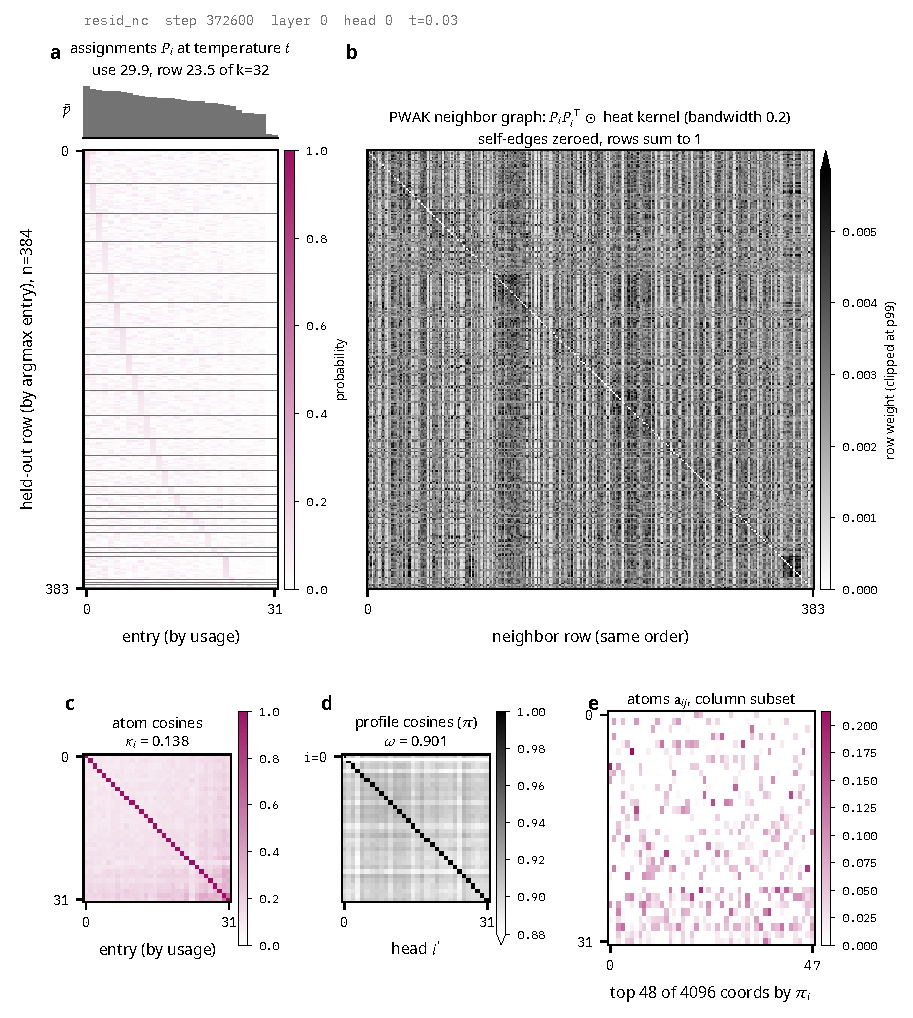
\includegraphics[width=\linewidth]{figures/fig-anatomy-softmax.pdf}
\caption[One softmax head, block by block]{\textbf{One softmax head,
	block by block.} Diagnostic panels corresponding to
	Figure~\ref{fig:anatomy} for head 0 of layer 0 in \texttt{resid\_nc}
	(step 372{,}600, $t{=}0.03$, one seed) evaluated on $n{=}384$
	held-out tail rows. Overall usage is spread across entries (use
	$29.9$ of $k{=}32$), but each row receives a near-uniform mixture
	(row $23.5$ in (a)), so the neighbor graph in (b) closely resembles
	the heat kernel alone, forming hub columns rather than discrete
	blocks ($\kappa_i{=}0.138$, $\omega{=}0.901$, $e{=}4096$). As in
	Figure~\ref{fig:anatomy}, this model was trained without the
	graph-based auxiliary statistics.}
\label{fig:anatomy-softmax}
\end{figure}

When hard selection is enforced during training, this categorical
structure is directly visible at the individual sample level
(Figure~\ref{fig:assignmap}, \texttt{assignmap.py}). On both SONAR and
GPT-2, layer-0 heads of the straight-through stack assign each row to a
single entry (row $1.0$) while distributing the dataset across 14--30
effective entries (use), and rows that share a ground-truth label tend to
select the same entry: most Cebuano sentences map to a single entry in
each of the three SONAR heads shown, and most GPT-2 newline and space
tokens map to a single entry per head. By contrast, a
$k_{\mathrm{SAE}}{=}32$ $\topk$ SAE evaluated on the same inputs
distributes each row across 25--29 effective active latents and spreads
the displayed subset across 1{,}066--1{,}533 effective latents overall;
there, a label such as GPT-2 newlines appears as a set of co-firing
latents rather than a single discrete slot.

\begin{figure}[tp]
\centering
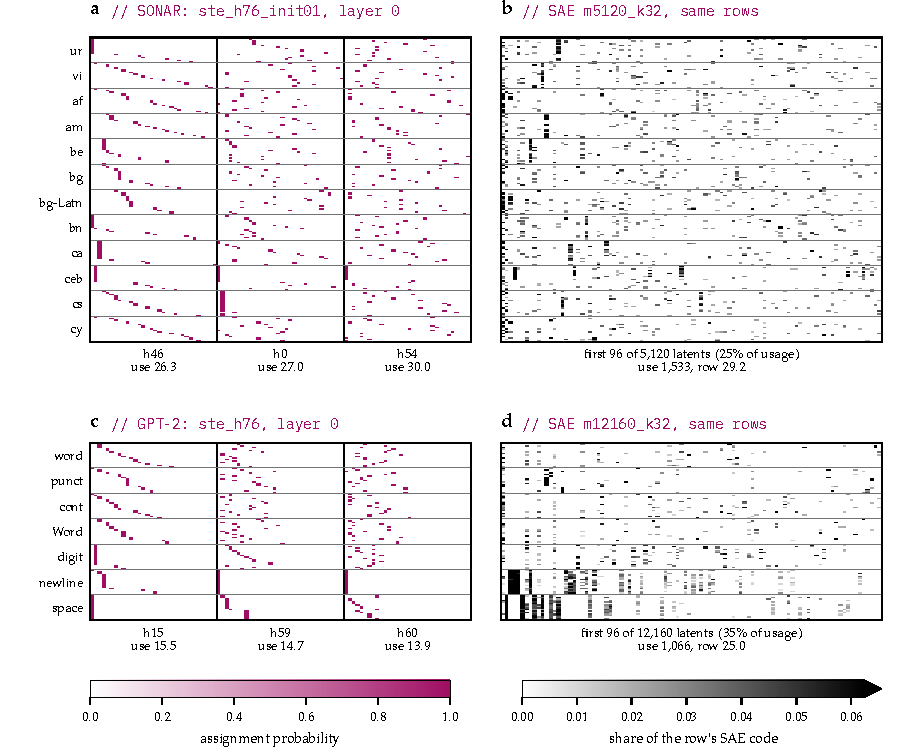
\includegraphics[width=\linewidth]{figures/fig-assignmap.pdf}
\caption[Hard codes against SAE codes, row by row]{\textbf{Hard codes
	against SAE codes, row by row.} Layer-0 assignments of the
	straight-through stacks on held-out tail rows (24 rows per label
	value, one seed per model) for the three heads with the highest
	null-adjusted NMI with the ground-truth label: (a) SONAR
	\texttt{ste\_h76\_init01} grouped by language, and (c) GPT-2
	\texttt{ste\_h76} grouped by token class. Entries are sorted by
	overall usage, and rows are grouped by label and ordered by their
	winning entries; each head's effective entry usage (use) is reported
	below, with per-row effective usage (row) equal to $1.0$. Panels (b)
	and (d) show the same rows in the same order encoded by a $\topk$ SAE
	trained on the corresponding cache (\texttt{m5120\_k32} and
	\texttt{m12160\_k32}), displaying each latent's share of a row's
	code across the 96 latents most used on these rows, with full-code
	use and row statistics reported below.}
\label{fig:assignmap}
\end{figure}

\subsection{Semantic coherence in detail}
\label{sec:coherence}

Under the whitened inner product that the training objective optimizes,
the softmax Ontologizer's mean within-head coherence $\zeta_{\cos}$ is
$-24.4$ (vs.\ $-17.6$ unwhitened, with the fraction of heads below $-2$
unchanged at $0.96$), the single-layer soft variant's mean is $-14.7$
(unchanged), and the single-layer hard variant's mean is $+179.3$ (vs.\
$+161.3$ unwhitened).

Only two heads in the reference softmax model (\texttt{resid\_nc})
exhibit positive clustering rather than repulsion: head 25 in layer 2
($\zeta_{\cos}{=}{+}346$) and head 28 in layer 3
($\zeta_{\cos}{=}{+}280$), followed by heads in the partially frozen
layer 4. Sampled entries from these heads also decode to generic text,
pointing to partial head collapse---entries that failed to differentiate
during training---rather than genuine semantic coherence; we have not
inspected them further.

Measuring within-head coherence via text similarity of plain autointerp
summaries is uninformative because roughly 77\% of Ontologizer entries
and 49\% of $k_{\mathrm{SAE}}{=}32$ SAE latents receive generic
summaries, inflating the permutation null (yielding $\zeta{=}{+}0.14$ for
Ontologizer heads). Switching to contrastive descriptions recovers a
modest signal: within-head description similarity exceeds the
head-membership permutation null for the softmax Ontologizer
($\zeta{=}{+}2.03$ across 155 within-head pairs), is marginal for the
single-layer hard variant ($\zeta{=}{+}1.55$, 62 pairs), and is weaker
still for the single-layer soft variant ($\zeta{=}{+}1.09$, 217 pairs).
Combined with the geometric results, this matches the pattern expected
for mutually exclusive values of a shared attribute: decoded entry
directions within an Ontologizer head repel one another geometrically
while their contrastive descriptions weakly cohere. This metric is also
the first to separate the stacked softmax Ontologizer from its
single-layer soft counterpart, although the evidence remains suggestive
given the limited sample coverage (a single global $\zeta$ per model
computed over the sampled features).

\subsection{Heads as communities of their input}
\label{sec:modularity}

Each head partitions its layer's input distribution into soft cells. To
test whether these cells align with local neighborhoods of that
input---concentrating more pairwise affinity within cells than expected
under a degree-preserving null graph---we compute soft modularity
(Eq.~\eqref{eq:modularity}) relative to size-matched random regroupings
of the same entries (Figure~\ref{fig:modularity}, using one checkpoint
per model). We compare the softmax Ontologizer \texttt{bl\_ctl\_full}
against two Matryoshka SAEs, \texttt{m5120\_g160top1\_p5} (trained heads)
and \texttt{m5120\_k32\_p5} (discovered groups), as well as their flat
counterparts \texttt{m5120\_g160top1} and \texttt{m5120\_k32}.

On the raw input graph itself, none of the models form modular
communities: layer 0 of the Ontologizer reaches $1.25\times$ its null
modularity, while every SAE sits between $0.76\times$ and $1.06\times$.
When each deeper layer is evaluated on its own residual input, however,
layers 1--4 of the Ontologizer achieve $2.1$--$2.9\times$ the modularity
of random entry regroupings. By contrast, Matryoshka SAEs evaluated on
matched prefix-residual graphs remain at chance, whether using trained
heads ($0.96$--$1.06\times$) or post hoc discovered groups
($0.88$--$1.03\times$ across blocks with sufficient coverage). Thus,
residual modularity does not arise merely from evaluating on residual
graphs or from imposing coarse-to-fine prefix losses on a head-structured
dictionary. Instead, the key distinction is that each Ontologizer layer
directly classifies the residual on which it is evaluated, whereas a
Matryoshka block is encoded from the original input and only trained to
reconstruct that residual. Because unnormalized modularity increases with
depth in both the learned partitions and the nulls (reaching $0.218$ vs.\
$0.105$ in layer 4) as assignments sharpen and residual graphs become
more clustered, the null-normalized ratio provides the appropriate
cross-layer comparison. Finally, low modularity on the raw input is
consistent with a factorial representation: a head that isolates one of
many independent factors cuts across nearest-neighbor structure in the
full embedding space, since nearby inputs share most factors without
necessarily sharing the one selected by that head.

\begin{figure}[tp]
\centering
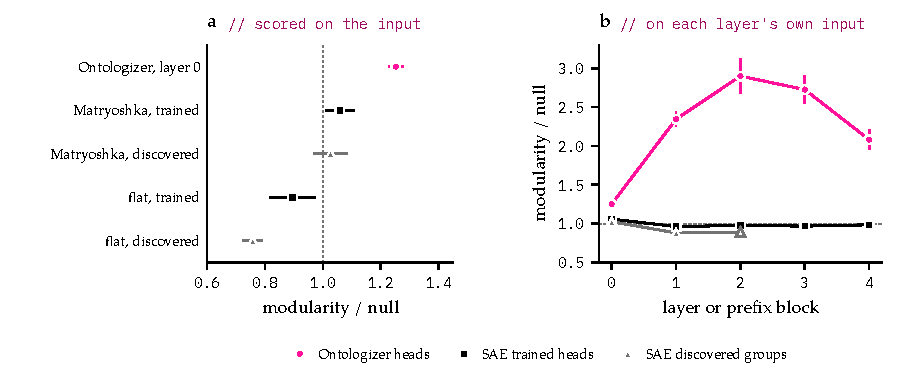
\includegraphics[width=\linewidth]{figures/fig-modularity.pdf}
\caption[Head partitions as communities of their input]{\textbf{Ontologizer
	heads form communities on the residual they classify, whereas SAE
	heads and groups do not.} Ratio of soft modularity to its
	size-matched regrouping null (\texttt{headstruct.py --modularity},
	Eq.~\eqref{eq:modularity}; one checkpoint per model), with error bars
	indicating $\pm2$ null standard deviations. (a) Models evaluated on
	the unreduced input graph: layer 0 of the softmax Ontologizer, block
	0 of the two Matryoshka SAEs (evaluated on the centered encoder input
	$\mathbf{x}-\mathbf{b}_{\mathrm{dec}}$), and the two flat SAEs. (b)
	Modularity ratio across depth, evaluating each layer or prefix block
	on the affinity graph of its own residual input. Hollow markers
	denote blocks whose discovered groups cover fewer than 10\% of
	samples; blocks 3 and 4 for discovered groups are omitted because
	block 3's null lies within two standard deviations of zero (3\%
	coverage) and block 4 contains only a single group, which its null
	reproduces identically.}
\label{fig:modularity}
\end{figure}

\subsection{Feature reliability}

Even in standard SAEs, individual latents are only partially reproducible
across random seeds. Comparing two $k_{\mathrm{SAE}}{=}32$ runs trained
with identical architectures and data from different initializations
(\texttt{k32} vs.\ \texttt{k32\_s43}, achieving $\fvu = 0.4994$ vs.\
$0.4967$), the fraction of latents with a cross-seed match is $0.31$,
$0.24$, $0.15$, and $0.03$ at activation-containment thresholds
$\tau = 0.3$, $0.5$, $0.7$, and $0.9$, respectively; at moderate
containment ($\tau{=}0.5$), roughly three quarters of individual latents
fail to reproduce across initializations. Comparing across dictionary
widths (\texttt{k32} $\to$ \texttt{m11264\_k32}), 190 of 5{,}114 active
parent latents split at $\tau{=}0.7$ (with a median of 3 child latents,
$0.37$ union coverage, and $0.42$ child overlap), alongside 441 geometric
twins and a heavy-tailed nearest-neighbor decoder-direction cosine
distribution (median $0.234$ vs.\ $0.119$ for random directions). Feature
splitting is therefore present, though topical co-firing remains the more
prominent organizational pattern. For an unsupervised steering-vector
generator, however, the relevant unit of reproducibility is the
head-level partition rather than an isolated feature vector;
Section~\ref{sec:seeds} evaluates partition reproducibility in the
hard-code Ontologizer and shows that it is substantially lower than
cross-seed latent matching in SAEs.

\subsection{Text-space fidelity (collateral ceiling)}
\label{sec:textfid}

\begin{table}[htbp]\centering\small
\begin{tabular}{@{}lrrr@{}}
\toprule
model & chrF & exact & NLL (ceiling 1.560, floor 3.999) \\
\midrule
corpus-mean floor & 0.176 & 0 & 3.999 \\
k32 tier (incl.\ p5, m11264) & 0.23 & 0.00 & 3.16--3.18 \\
k32\_bl          & 0.204 & 0.00 & 3.365 \\
k160 / g160top1  & 0.27--0.28 & 0.00 & 2.41--2.43 \\
onto soft        & 0.552 & 0.070 & 1.585 (gap 0.025) \\
g160softmax      & 0.591 & 0.094 & 1.568 (gap 0.008) \\
k5120            & 0.841 & 0.562 & 1.560 (gap 0.000) \\
\bottomrule
\end{tabular}
\caption{Downstream text fidelity on 512 held-out tail rows under forced
English decoding. The NLL ceiling ($1.560$) is shared across all models
and corresponds to scoring the unperturbed embedding's decode under the
unperturbed embedding.}
\end{table}

The relationship between $\fvu$ and decoded text fidelity is strongly
nonlinear: reconstructions at $\fvu \approx 0.5$ decode to text that
preserves rough topic while altering factual content, scoring only
slightly above the corpus-mean floor, whereas both the softmax
Ontologizer and \texttt{g160softmax} remain close to the likelihood
ceiling and preserve nearly all decodable content. Across the eleven
Ontologizer runs for which both metrics were evaluated (spanning the
selection-rule sweep and the straight-through arms in
Table~\ref{tab:steerfid}), downstream ``loss recovered'' is strictly
monotonic in $\fvu$ (Spearman rank correlation $-1$). Text-space fidelity
therefore confirms that the whitened embedding objective transfers
monotonically to decoded text rather than defining an independent
performance axis. This baseline fidelity is particularly consequential
for steering: a steering primitive routed through a sparse reconstruction
that fails to preserve text (including the entire
$k_{\mathrm{SAE}}{\leq}160$ SAE tier) starts from roughly $0.75$
collateral before any intervention is applied, whereas the dense-mixture
classifier codes start near zero.

\subsection{Concept (language) localization}
\label{sec:langlocal}

\begin{table}[htbp]\centering\small\setlength{\tabcolsep}{4pt}
\begin{tabular}{@{}lrrrrrr@{}}
\toprule
& \multicolumn{3}{c}{86 languages} & \multicolumn{3}{c}{five languages, F1@1} \\
\cmidrule(lr){2-4}\cmidrule(l){5-7}
model & F1@1 & F1@4 & F1@16 & own tags & \stackhead[r]{it pt\\nl ja} & \stackhead[r]{ca ro\\sv ko} \\
\midrule
k160             & 0.119 & \textbf{0.393} & \textbf{0.473} & 0.684 & 0.841 & 0.841 \\
k32 ($m{=}5120$) & 0.089 & 0.347 & 0.465 & 0.624 & 0.868 & 0.876 \\
m11264\_k32      & 0.078 & 0.364 & 0.471 & 0.551 & 0.860 & 0.871 \\
k32\_bl          & 0.084 & 0.228 & 0.368 & 0.695 & 0.840 & 0.786 \\
k32\_p5          & 0.061 & 0.322 & 0.456 & 0.625 & 0.862 & 0.870 \\
g160top1         & 0.066 & 0.207 & 0.302 & 0.592 & 0.542 & 0.700 \\
g160softmax      & 0.067 & 0.162 & 0.328 & 0.432 & 0.437 & 0.433 \\
k5120            & 0.064 & 0.130 & 0.237 & 0.439 & 0.448 & 0.447 \\
softmax Ontologizer (entries) & 0.022 & 0.022 & 0.135 & 0.333 & 0.333 & 0.333 \\
hard-code stack (entries) & \textbf{0.121} & 0.153 & 0.362 & 0.685 & 0.804 & 0.806 \\
hard-code flat (entries) & 0.120 & 0.141 & 0.319 & 0.609 & 0.798 & 0.703 \\
\bottomrule
\end{tabular}
\caption{Language localization (\texttt{langprobe.py}): held-out
one-vs-rest macro F1 of the single best latent and of logistic probes on
the best 4 and 16 latents across tail rows. The first three columns
evaluate all 86 languages, where the always-positive baseline scores
$0.023$ and a dense linear probe on the raw embedding scores $0.676$. The
final three columns report single-latent macro F1 within three
five-language subsets, where the always-positive baseline scores $0.333$:
English, French, Spanish, German, and Chinese, which were encoded under
their own SONAR source tags (Appendix~\ref{app:data}), alongside two
composition-matched subsets encoded under the English tag. The softmax
Ontologizer is \texttt{resid\_nc}, and the hard-code models are
\texttt{ste\_h76\_init01} and \texttt{ste\_l1\_h380\_i01}.}
\label{tab:langlocal}
\end{table}

Language identity remains distributed across features in every model
(Table~\ref{tab:langlocal}): the highest single-latent macro F1 is
$0.121$, compared to a dense-probe ceiling of $0.676$ (script-distinctive
languages such as Chinese reach roughly $0.98$ from a single latent,
whereas languages sharing a script overlap heavily). Individual entry
probabilities in the softmax Ontologizer do not localize language at all,
remaining at the always-positive baseline at both 1 and 4 entries. By
contrast, the hard-code models' one-hot entries match the best SAE at a
single entry ($0.121$ and $0.120$ vs.\ $0.119$), though they trail at 4
and 16 entries. Under a single-feature SAE lens, the soft code's baseline
score appears uninformative; under a categorical-classifier lens,
however, a soft head encodes a factor in its \emph{assignment}
distribution rather than in any single entry's scalar probability.
Consistent with this view, partition-level analysis of \texttt{resid\_nc}
identified layer-1 heads whose partitions carry mutual information with
script and language family, including one entry (entry 17 of head 8 in
layer 1) causally verified to produce Burmese decodes. Evaluating head
partitions directly with \texttt{headlang.py} on a configuration-matched
softmax reference and on the hard-code arms (Section~\ref{sec:lang})
shows that the softmax reference's strongest head reaches a
null-corrected NMI of only $0.043$, roughly one quarter of the hard
code's peak. Even in the hard-code stacks, language information is
distributed weakly across many heads' partitions rather than concentrated
in a few: across both seeds, the 76 most language-informative heads out
of 380 are precisely the 76 heads in layer 0 (\texttt{headlang.py}), with
the strongest head reaching roughly one fifth of the maximum attainable
NMI, every deeper head scoring below all layer-0 heads, and removing the
top 32 heads leaving most of the recoverable language signal intact in
the rest of the code (Appendix~\ref{sec:langdetail}).

\paragraph{What the English tag does to localization.} Because most of
the SONAR cache was encoded under the English source-language tag
(Appendix~\ref{app:data}), this tagging artifact strongly shapes
Table~\ref{tab:langlocal}. Each $\topk$ SAE learns a single latent that
fires jointly on French, Spanish, and German---the three Latin-script
languages encoded under their own source tags---separating them from the
English-tagged remainder without distinguishing them from one another
(yielding F1@1 near $0.49$ for each, vs.\ $0.03$--$0.15$ for Italian,
Portuguese, Dutch, Catalan, Romanian, and Swedish). When evaluation is
restricted to the five correctly tagged languages, neither French nor
German has a dedicated latent or entry in any model (best F1@1 of
$0.39$--$0.50$ vs.\ the $0.33$ baseline), whereas English ($0.64$--$0.96$)
and Chinese ($0.86$--$0.997$ in the sparse SAEs and hard codes) do.
Moreover, five-language subsets of matching composition that were encoded
under the English tag achieve higher single-latent localization (macro
F1@1 of $0.70$--$0.88$ vs.\ $0.55$--$0.70$ for the correctly tagged
subset) in every model except \texttt{g160top1} and the dense codes, even
though a dense linear probe separates the correctly tagged subset at
least as accurately ($0.95$--$1.00$ vs.\ $0.92$--$0.98$), indicating that
each English-tagged Latin-script language carries a distinct signature.
Consequently, most single-latent localization among Latin-script
languages in this cache reflects source-tag mismatch rather than
intrinsic language separation; whether dictionaries trained on
consistently tagged embeddings would allocate dedicated latents to those
languages remains untested.

Entry-level enrichment tests the same relationship at the granularity of
individual (entry, label) cells (Figure~\ref{fig:enrich},
\texttt{enrich.py}). In \texttt{resid\_nc}, 3{,}698 of 226{,}763 tested
(entry, language) cells are statistically significant at FDR $0.05$, and
label alignment is concentrated almost entirely in layer 0: the highest
null-adjusted head NMI is $0.050$ in layer 0, compared to $0.006$,
$0.003$, $0.002$, and $0.001$ across layers 1--4. The GPT-2 hard code
exhibits the same concentration in layer 0 for both token class ($0.149$
in layer 0 vs.\ at most $0.029$ in deeper layers, with 11{,}777 of
53{,}412 tested (entry, token class) cells significant) and token
position ($0.105$ in layer 0 vs.\ at most $0.011$ in deeper layers).

\begin{figure}[tp]
\centering
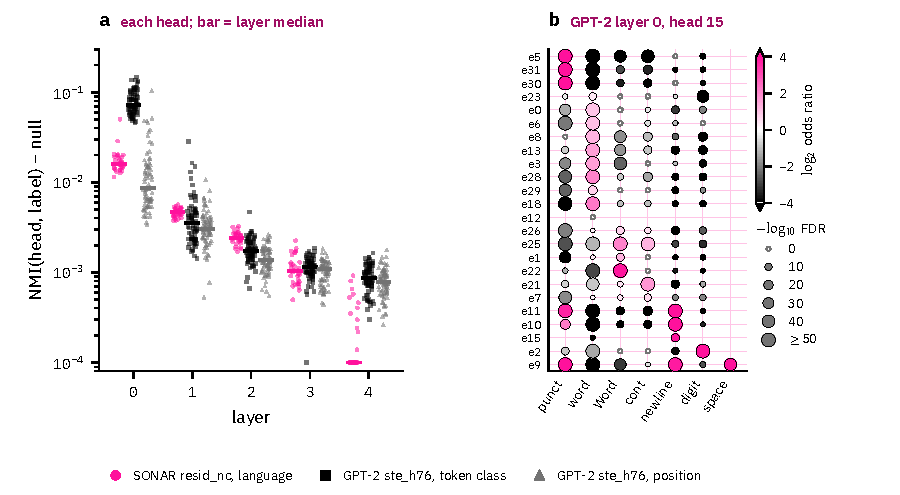
\includegraphics[width=\linewidth]{figures/fig-enrich.pdf}
\caption[Label structure by layer]{\textbf{Label structure is concentrated
	in layer 0.} (a) NMI between each head's winning entry and a
	ground-truth label on the held-out tail, minus the mean across five
	label-shuffled permutations, showing one point per head (values at or
	below the null mean are plotted at $10^{-4}$) and horizontal bars at
	each layer's median: SONAR \texttt{resid\_nc} against language, and
	GPT-2 \texttt{ste\_h76} against token class and token position. (b)
	Enrichment across entries and token classes for the GPT-2 layer-0 head
	with the highest token-class NMI (head 15): marker color encodes the
	Haldane-corrected $\log_2$ odds ratio, marker area encodes
	$-\log_{10}$ FDR (capped at 50), and filled circles indicate FDR
	$<0.05$, with entries grouped by the token class for which they are
	most enriched. One seed per model.}
\label{fig:enrich}
\end{figure}

\subsection{Shrinkage decomposition}

Standard $\topk$ SAEs exhibit very small magnitude error: refitting
unconstrained least-squares coefficients on each sample's frozen active
support reduces pre-refit $\fvu$ by only $2.2$--$2.4\%$ for the
$k_{\mathrm{SAE}}{=}32$ variants, $8.5\%$ for \texttt{k160}, $0.6\%$ for
the bilinear SAE (\texttt{k32\_bl}), and $1.9\%$ for the Matryoshka SAE
(\texttt{k32\_p5}). Similarly, \texttt{g160top1} is nearly perfectly
calibrated ($0.3\%$ reduction), indicating that its reconstruction gap
stems purely from support selection. For the softmax Ontologizer's
truncated deviation codes, support-frozen refitting removes $16\%$ of the
error at $\nu{=}1$ and $33\%$ at $\nu{=}2$, matching the fraction
$\lvert\mathcal{S}\rvert / d$ ($160/1024$ and $320/1024$ across
\texttt{resid\_nc}'s $5\times32$ heads) that any $\lvert\mathcal{S}\rvert$
unconstrained coefficients would remove from an isotropic whitened
residual. Indeed, size-matched random supports remove slightly more error
than the models' chosen supports: $19\%$ and $36\%$ for the Ontologizer
($\nu$ random entries per head), and $20\%$, $13\%$, and $4.6\%$ for
\texttt{k160}, \texttt{g160top1}, and \texttt{k32}, compared to $8.5\%$,
$0.3\%$, and $2.2\%$ on their own supports (\texttt{refit.py}; supports
of size $\geq d$ are excluded as underdetermined). Because no model's
active support benefits more from refitting than a random support of equal
size, there is no evidence that the pin-and-renormalize truncation rule
mis-scales the retained entries.

Separately, comparing non-adaptive truncation (freezing the soft
assignments $P$ from a clean forward pass, truncating them, and decoding
linearly) against in-forward truncation (allowing deeper layers to
reclassify the residual left by truncated earlier layers) reveals a large
gap at $\nu{=}8$, reducing $\fvu$ from $0.268$ to $0.094$---nearly a
threefold improvement from downstream compensation. Alongside the larger
depth effect measured in Section~\ref{sec:depth}, this adaptive
re-encoding has direct implications for steering: deeper layers actively
compensate for edits to earlier codes, providing robustness to small
perturbations while also inducing widespread downstream collateral flips
(Section~\ref{sec:entangle}).

\subsection{Steering through the text round trip}
\label{sec:steertext}

Table~\ref{tab:steerfid} reports text-space reconstruction fidelity and
text-cycle steering across the Ontologizer selection-rule sweep, the
straight-through arm, and the $k_{\mathrm{SAE}}{=}32$ SAE, evaluated on 64
features per run.

\begin{table}[htbp]\centering\small\setlength{\tabcolsep}{4pt}
\begin{tabular}{@{}lrrrrrrrr@{}}
\toprule
run & $\fvu$ & chrF & loss rec. & net @0.25 & @0.5 & @1.0 & hit @1.0 & rand.\ hit \\
\midrule
top8          & 0.0370 & 0.416 & 0.941 & 0.203 & 0.404 & \textbf{0.652} & 0.734 & 0.359 \\
top2          & 0.3516 & 0.246 & 0.521 & 0.072 & 0.277 & 0.509 & 0.578 & 0.109 \\
top16         & 0.0052 & 0.557 & 0.987 & 0.027 & 0.110 & 0.363 & 0.381 & 0.156 \\
top4\_shm     & 0.0761 & 0.375 & 0.892 & 0.112 & 0.140 & 0.248 & 0.242 & 0.062 \\
softmax\_shm  & 0.0007 & 0.706 & 0.997 & 0.058 & 0.128 & 0.242 & 0.211 & 0.094 \\
top2\_shm     & 0.1911 & 0.301 & 0.742 & 0.018 & 0.071 & 0.196 & 0.150 & 0.016 \\
top8\_shm     & 0.0287 & 0.437 & 0.954 & $-0.015$ & 0.074 & 0.176 & 0.330 & 0.094 \\
top1          & 0.7190 & 0.170 & 0.126 & 0.047 & 0.104 & 0.064 & 0.102 & 0.109 \\
\texttt{ste\_h76} & 0.2293 & 0.295 & 0.695 & 0.033 & 0.045 & $-0.020$ & 0.055 & 0.125 \\
\midrule
SAE \texttt{k32} & 0.4994 & 0.228 & 0.345 & 0.048 & 0.187 & 0.402 & 0.260 & 0.016 \\
\bottomrule
\end{tabular}
\caption{Text fidelity and text-cycle steering (\texttt{steerfid.py},
\texttt{--n-features 64}) across Ontologizer selection rules and the
$k_{\mathrm{SAE}}{=}32$ SAE under the same protocol. Net effect is feature
effect minus the random-direction control. An additional run
(\texttt{topk4\_rev}, $\fvu = 0.164$) achieves a net effect of $0.636$ at
magnitude $1.0$.}
\label{tab:steerfid}
\end{table}

Text-cycle steerability does not track reconstruction fidelity. The
strongest steerer is \texttt{top8} ($\fvu = 0.037$), whereas the most
faithful reconstruction model (\texttt{softmax\_shm}) achieves roughly one
third of its net steering effect, and every \texttt{\_shm} variant steers
roughly three times more weakly than its unregularized counterpart
(\texttt{top2} $0.509$ vs.\ \texttt{top2\_shm} $0.196$; \texttt{top8}
$0.652$ vs.\ \texttt{top8\_shm} $0.176$). The straight-through arm
(\texttt{ste\_h76}) exhibits the weakest response of all: its unadjusted
effect remains flat across step magnitudes ($0.018$, $0.014$, and $0.027$)
and no larger than a random perturbation, while its hit rate ($0.055$)
falls below its random-direction control ($0.125$). Under the same
protocol, the $k_{\mathrm{SAE}}{=}32$ SAE shows a clear text-cycle effect
(net effect $0.402$ at magnitude $1.0$, with a hit rate of $0.260$ vs.\
$0.016$ for random directions).

Two methodological caveats limit this evaluation. First, sampling 16
features is too noisy to support reliable estimates, and even at 64
features the straight-through arm's net effect changes sign depending on
the random control draw (shifting from negative at all magnitudes on 16
features to $+0.033$, $+0.045$, and $-0.020$ at 64 features), indicating
that its text-cycle signal lies within measurement noise. Second, hit
rates are not directly comparable between hard and soft codes: because
hard-code activations are binary ($0$ or $1$), recording a hit requires
that the re-encoded argmax land on the exact target entry, whereas a soft
code need only exceed a fractional activation threshold.

\paragraph{The text cycle is too weak to support conclusions.} Evaluated
on an \emph{unsteered} round trip across the final 512 cache rows,
decoding and re-encoding preserves partial semantic similarity to the
source row ($\cos\angle(\mathbf{x}, \mathrm{cycle}(\mathbf{x})) = 0.382$,
vs.\ $0.091$ between unrelated rows) while shifting embeddings away from
the corpus distribution (mean cosine with the corpus mean drops from
$0.561$ on clean rows to $0.160$ after cycling). Crucially, the round trip
fails to preserve discrete head assignments: a head's winning entry
survives an unsteered cycle on only $12.9\%$ of rows in
\texttt{ste\_h76} and $10.8\%$ in the softmax model, compared to $3.1\%$
by chance, and in the hard code this survival rate drops sharply with
depth from $36.2\%$ in layer 0 to $4.8\%$ in layer 4. Even an ideal
code-level intervention could therefore register on at most roughly
$13\%$ of cycled examples, which is on the same order as the hit rates
reported by this evaluation. Several aspects of the cache protocol make
this round trip unusually lossy: cache rows correspond to 512-token
document openings---exceeding the sequence length at which SONAR
auto-encoding degrades---and are decoded into English regardless of source
language through a generator that is sensitive to small embedding
perturbations~\cite{lcmteam2024largeconceptmodelslanguage}. Thus, whereas
embedding-space reconstruction remains reliable, text generation obscures
most of the code-level signal.

\section{Supplementary results: training, reproducibility, and steering of the softmax Ontologizer}
\label{app:softdyn}

The experiments in this section originate from the project proposal's
evaluation suite and examine the training dynamics, cross-seed
reproducibility, and steering behavior of the softmax Ontologizer. Two
models appear throughout: \texttt{resid\_nc} (trained for 372{,}600
steps), which serves as the reference softmax model in the comparisons
above, and \texttt{resid\_nc\_hm}, which uses the same architecture and
hyperparameters plus the batch-mean uniformity term $\mathrm{KL}_m$
(weighted by $s_{\mathrm{KL}_m}$) and is trained for 4.38M steps. Unless
stated otherwise, evaluations of \texttt{resid\_nc\_hm} use its final
checkpoint.

\subsection{Head freezing and the batch-mean uniformity term}
\label{sec:freeze}

We classify a head as frozen when its largest entry usage share is at
least $0.95$ and its assignment churn is at most $0.02$. In
\texttt{resid\_nc}, the final layer (layer 4 of 0--4) begins freezing
near step 190k---well after temperature annealing concludes---reaching 27
of 32 heads by step 210k, peaking at 28, and remaining frozen at the final
checkpoint (Figure~\ref{fig:freeze}). As shown in
Section~\ref{sec:lastlayer}, this final layer becomes largely inert once
the prefix residual error is small, explaining why the freeze incurs
little reconstruction penalty. In \texttt{resid\_nc\_hm}, by contrast,
this late-stage freeze never occurs. Instead, the model undergoes only a
brief early annealing transient---peaking at step 10k with 22 of 32 frozen
heads in layer 1, alongside 16, 11, and 4 of 32 in layers 2, 3, and
0---that resolves completely by step 30k, leaving all layers unfrozen at
the final checkpoint. Including the batch-mean uniformity term
$\mathrm{KL}_m$ therefore prevents late-stage head freezing.

\begin{figure}[htbp]\centering
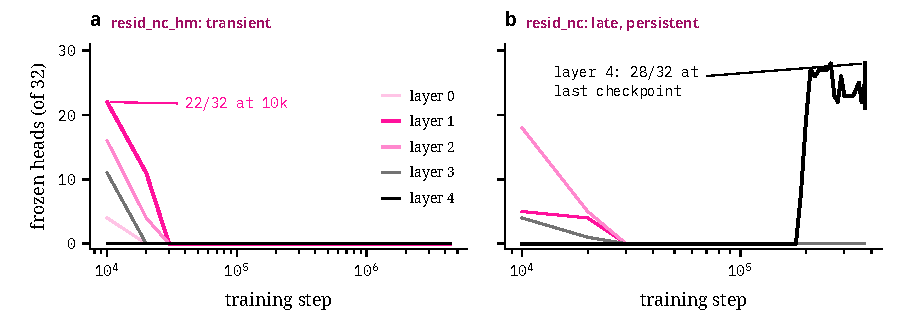
\includegraphics[width=\linewidth]{figures/fig-freeze.pdf}
\caption{Frozen heads per layer over training. (a)
\texttt{resid\_nc\_hm}, trained with the batch-mean uniformity term
$\mathrm{KL}_m$, exhibits only an early annealing transient, peaking at
22/32 frozen heads in layer 1 at step 10k and recovering to zero across
all layers by step 30k. (b) \texttt{resid\_nc} develops a persistent
post-annealing freeze in layer 4 starting near step 190k that continues
through its final checkpoint.}
\label{fig:freeze}
\end{figure}

Four 372k-step retrains of the \texttt{resid\_nc\_hm} configuration---an
unmodified control and three single-hyperparameter variants---isolate the
source of the early transient (Figure~\ref{fig:variants}). The control
reproduces the transient closely (22/32 frozen heads in layer 1 at step
10k, recovering to zero everywhere by step 30k) and exhibits no late
freeze. Extending the temperature annealing schedule from 50k to 150k
steps lowers and broadens the transient (peaking at 14/32 in layer 1 at
step 30k and clearing by step 50k). By contrast, raising winner dropout
from $0.1$ to $0.25$ tracks the control to within two heads at the peak,
and holding the logit-noise floor constant at its initial value leaves the
trajectory unchanged. Thus, the early transient is governed by the
temperature schedule alone, and every retrain finishes completely
unfrozen.

\begin{figure}[htbp]\centering
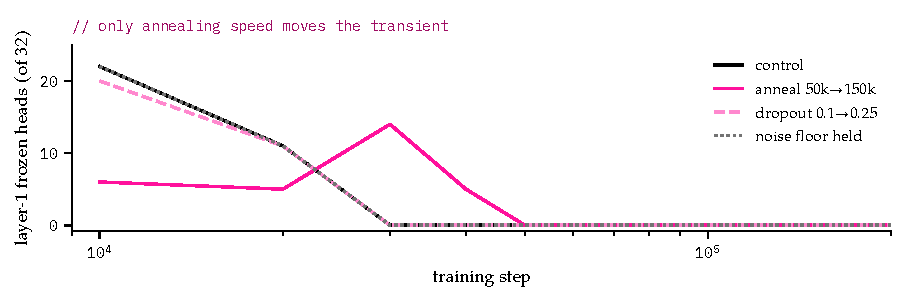
\includegraphics[width=\linewidth]{figures/fig-variants.pdf}
\caption{Layer-1 frozen head counts during the early transient across four
372k-step retrains of \texttt{resid\_nc\_hm}. Holding the logit-noise
floor constant overlaps the control curve identically, and raising winner
dropout tracks it to within two heads at the peak; only extending the
temperature annealing schedule shifts the curve, trading peak height for
duration.}
\label{fig:variants}
\end{figure}

\paragraph{An HSIC penalty in place of the auxiliary losses.} These
variants are motivated by the HSIC bottleneck~\cite{ma2020hsic}, which
trains layers without backpropagation to minimize dependence on their
inputs while maximizing dependence on ground-truth labels, both measured
by normalized HSIC. Because an autoencoder's target is its own input,
those two objectives collapse into one and neither is used directly here;
instead, reconstruction continues to optimize whitened MSE while a single
kernel penalty discourages statistical dependence among heads within a
layer. Two 372k-step arms on the \texttt{resid\_nc\_hm} configuration
penalize inter-head dependence via the pairwise head CKA of
Section~\ref{sec:hsic} computed under the biased
estimator~\cite{gretton2005}: one arm replaces the four standard auxiliary
terms with the CKA penalty, and the other adds the CKA penalty to them.
Replacing the auxiliary terms severely degrades head utilization: a
persistent late freeze overtakes 77 of 160 heads by the final checkpoint,
including all 32 heads of layer 3 from step 80k onward, while tail-mean
training MSE lands slightly behind the control ($3.7\times10^{-5}$ vs.\
$3.4\times10^{-5}$). Adding the penalty alongside the auxiliary terms
performs worse on both metrics, yielding a training MSE of
$4.4\times10^{-5}$ and leaving 41 of 160 heads frozen at completion after
layer 3 freezes completely by step 80k and only partially recovers
(Figure~\ref{fig:hsicbottleneck}).

This failure reflects the late-stage freezing mode seen in
\texttt{resid\_nc} rather than the early annealing transient, and it stems
directly from estimator bias. Because the biased CKA floor between
independent heads decreases with the number of active entries and vanishes
for a frozen head (Section~\ref{sec:hsic}), the optimizer can reduce the
penalty simply by concentrating or freezing heads, placing the penalty in
direct opposition to the batch-mean uniformity term $\mathrm{KL}_m$.
Retrained on the current codebase, the replacement arm reproduces this
freeze step for step (freezing 6, 29, and 32 of 32 heads in layer 3 at
steps 60k, 70k, and 80k, vs.\ 7, 29, and 32 originally) while its summed
CKA penalty drops by 80\%. Under the unbiased estimator, by contrast, the
same arm freezes at most 5 heads---all in layer 4---through 93k steps (one
seed per arm). Once estimator bias is removed, however, the inter-head CKA
penalty has very little residual dependence to act upon, and whether it
could replace the standard auxiliary terms over a full training run
remains untested.

\begin{figure}[htbp]\centering
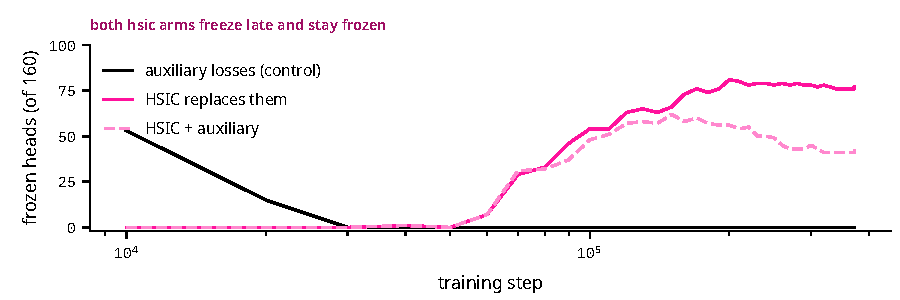
\includegraphics[width=\linewidth]{figures/fig-hsic.pdf}
\caption{Total frozen heads across all layers over 372k training steps
for three loss configurations based on \texttt{resid\_nc\_hm}. The
auxiliary-loss control exhibits only the brief early transient before
recovering, whereas both HSIC arms---whose head-CKA penalty uses the
biased estimator---develop a persistent late-stage freeze that the
standard auxiliary terms only partially mitigate.}
\label{fig:hsicbottleneck}
\end{figure}

\subsection{Development over training}
\label{sec:devinterp}

Tracking \texttt{resid\_nc\_hm} across all 448 saved checkpoints applies
the $z$-score coherence evaluation of Section~\ref{sec:prelim-orth} to
least-squares refitted end-to-end directions rather than to raw decoded
dictionary atoms. These two quantities are not directly comparable: raw
decoded atoms in \texttt{resid\_nc} repel one another
($\zeta_{\cos}{=}{-}17.6$), whereas refitted end-to-end directions at the
final checkpoint of \texttt{resid\_nc\_hm} cohere strongly
($\zeta_{\cos}{=}{+}72$), reflecting differences in both model and
measurement (since the end-to-end refit incorporates the shared decoder
and cross-layer interactions). Moreover, because a head's directions are
determined by the model's function only up to a shared per-head offset
(Section~\ref{sec:prelim-orth}), the trained parameters and a
least-squares refit fix that offset differently. Under the refitted
metric, coherence rises, peaks, and partially relaxes over training
(Figure~\ref{fig:devinterp}): mean within-head $\zeta_{\cos}$ increases
from $1.8$ at step 10k to a peak of $119$ near step 370k (median $123$,
with every head exceeding $\zeta_{\cos}{=}2$), before relaxing over the
subsequent 4M steps to $72$ at the final checkpoint (median $105$, with a
fraction $0.79$ of heads above $\zeta_{\cos}{=}2$). Meanwhile, the
assignments
themselves move in the opposite direction once the early annealing
transient resolves: mean per-sample entropy returns to $4.5$ out of the
5-bit maximum, and batch-mean KL divergence approaches zero. Relative to
initialization, training therefore consolidates the geometry written by
the assignments while the assignments themselves remain soft.

\begin{figure}[htbp]\centering
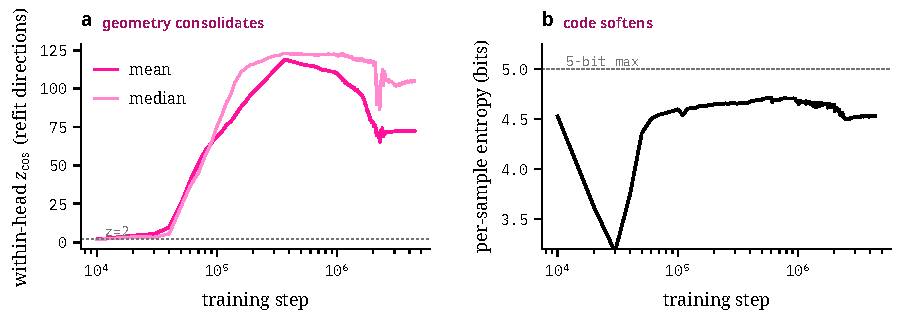
\includegraphics[width=\linewidth]{figures/fig-devinterp.pdf}
\caption{Training trajectory across all 448 saved checkpoints of
\texttt{resid\_nc\_hm}. (a) Within-head coherence of refitted end-to-end
directions, standardized against size-matched nulls, showing an initial
rise, a peak near step 370k, and subsequent partial relaxation. (b) Mean
per-sample assignment entropy, which returns toward the 5-bit maximum
following the early annealing transient.}
\label{fig:devinterp}
\end{figure}

Evaluated at the individual entry level on a single seed of
\texttt{resid\_nc}, dictionary directions stabilize after temperature
annealing concludes (Figure~\ref{fig:entrydrift}, \texttt{entrydrift.py}).
Across layers 0--3, the median cosine similarity between an active entry's
decoded atom and its final-checkpoint direction rises from $0.40$--$0.51$
at step 10k to $0.73$--$0.82$ at step 60k (immediately after annealing),
reaching $0.99$--$1.00$ from step 320k onward. By contrast, layer 4 begins
at $0.23$, plateaus near $0.53$ between steps 60k and 160k, and converges
only after freezing near step 190k (Section~\ref{sec:freeze}), retaining
142 active entries out of 1{,}024. Entry utilization instead dips
temporarily at the end of annealing: $40\%$ of layer-0 entries fall below
the usage threshold at step 60k, though all but $7\%$ recover by the end
of training.

\begin{figure}[tp]
\centering
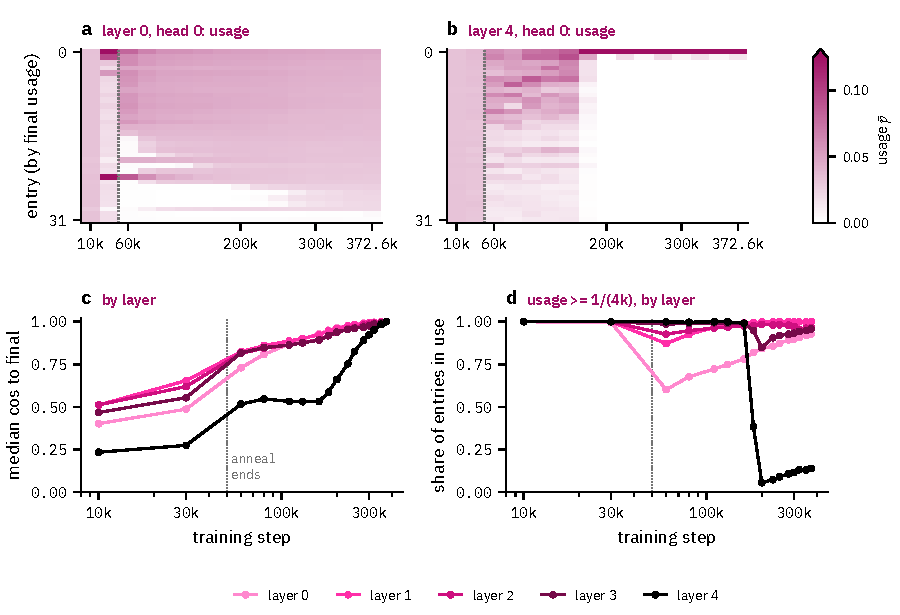
\includegraphics[width=\linewidth]{figures/fig-entrydrift.pdf}
\caption[Entry drift over training]{\textbf{Entries stabilize after
	temperature annealing.} Trajectory across the 16 retained checkpoints
	of \texttt{resid\_nc} on the held-out tail (one seed). (a, b) Mean
	usage $\bar{p}_{ij}$ across the 32 entries of head 0 in layers 0 and
	4, with one column per checkpoint (not spaced linearly in step) and
	entries ordered by final usage; the vertical dotted line marks the
	end of temperature annealing. (c) Median cosine similarity per layer
	between each active entry's decoded atom and its final direction,
	computed over entries active at the final checkpoint. (d) Fraction of
	active entries per layer ($\bar{p}_{ij}\geq 1/4k$).}
\label{fig:entrydrift}
\end{figure}

\subsection{Scaling: a star sweep}
\label{sec:starsweep}

To test whether within-head coherence improves with model scale, we
trained a seven-point star sweep around the baseline $h{=}32$, $k{=}32$,
$l{=}5$ architecture, varying one hyperparameter axis at a time for 4
epochs (62k steps, vs.\ 372k in the standard retrain schedule). None of
the swept axes produce an increase in coherence
(Figure~\ref{fig:scaling}): coherence shows no positive association with
parameter count (Spearman correlation $+0.14$ for mean $\zeta_{\cos}$ and
$-0.54$ for the fraction of heads above $\zeta_{\cos}{=}2$), entry-usage
imbalance increases with scale (Spearman $+0.86$), and the clearest
single-axis trend runs opposite to the hypothesis, with mean
$\zeta_{\cos}$ decreasing monotonically as the number of entries per head
grows ($20.2$, $6.3$, and $3.7$ at $k = 16$, $32$, and $64$). The widest
run ($h{=}64$) fails to converge within this training budget (exhibiting a
tail MSE $20\times$ higher than the other runs), so its low score is
uninformative. Overall, seven configurations trained on an abbreviated
schedule provide limited evidence in either direction; full-length scaling
runs remain a necessary control.

\begin{figure}[htbp]\centering
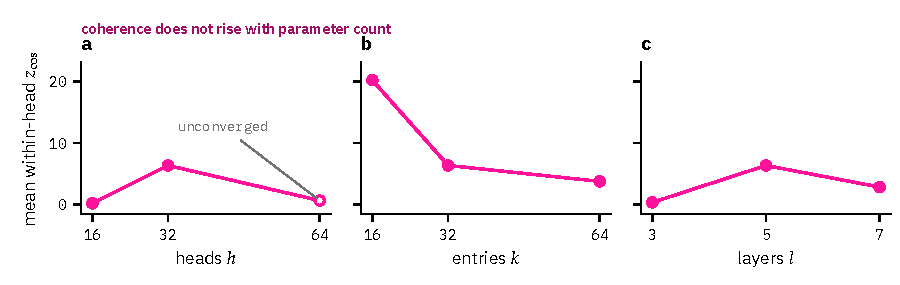
\includegraphics[width=\linewidth]{figures/fig-scaling.pdf}
\caption{Within-head coherence across each axis of the 4-epoch (62k-step)
star sweep: (a) heads $h$, (b) entries $k$, and (c) layers $l$. None of
the axes exhibit the predicted increase with scale, and coherence
decreases monotonically with $k$. The open marker in (a) denotes the
unconverged $h{=}64$ run.}
\label{fig:scaling}
\end{figure}

\subsection{Seed stability of soft partitions}
\label{sec:softseed}

Comparing a second independent seed of the \texttt{resid\_nc\_hm}
configuration against the primary run at a matched training budget (370k
steps each) reveals almost no cross-seed correspondence
(Figure~\ref{fig:softseed}): no pair of heads and at most $0.3\%$ of
individual atoms exceed a $0.3$ cosine threshold in dictionary geometry,
and activation-frame containment over a shared evaluation batch reaches at
most $0.001$ across all thresholds, compared to $0.31$, $0.24$, $0.15$,
and $0.03$ between the $k_{\mathrm{SAE}}{=}32$ SAE (\texttt{k32}) and its
seed replica at $\tau = 0.3$, $0.5$, $0.7$, and $0.9$. This near-zero
match is not due to metric insensitivity: comparing the primary run
against an earlier checkpoint of itself $2{,}600$ steps apart yields
$1.000$ geometric matching at every threshold and $0.65$ activation
containment at $\tau{=}0.3$ ($0.20$ at $\tau{=}0.9$). At matched training
steps, soft Ontologizer partitions are therefore less reproducible across
seeds than individual SAE latents, consistent with the partition-NMI and
output-contribution results for the straight-through arm in
Section~\ref{sec:seeds}. Training a second seed to the full 4.4M-step
horizon remains an open control.

\begin{figure}[htbp]\centering
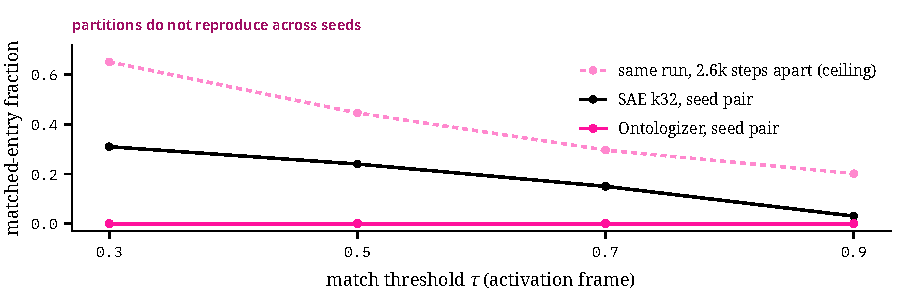
\includegraphics[width=\linewidth]{figures/fig-seed.pdf}
\caption{Cross-seed matched-entry fraction under activation-frame
containment across thresholds $\tau$. Comparing checkpoints from the same
run establishes the metric's detection ceiling ($0.65$ at $\tau{=}0.3$);
the $k_{\mathrm{SAE}}{=}32$ SAE pair reproduces partially, whereas the
softmax Ontologizer's entries show virtually no cross-seed matching.}
\label{fig:softseed}
\end{figure}

\subsection{Steering against supervised baselines}
\label{sec:steeroverlay}

On the final saved checkpoint of \texttt{resid\_nc\_hm} (step
4{,}380{,}000), a matched-budget language-steering evaluation compares
forced entries against supervised difference-of-means and linear-probe
vectors alongside a random-direction baseline
(Table~\ref{tab:steer-overlay}). As expected, each steering method
achieves the largest displacement when projected onto its own direction.
Along the shared difference-of-means direction, forcing an entry shifts
decoded embeddings $0.64\times$ as far as supervised difference-of-means
steering itself and $4.2\times$ as far as linear-probe steering. However,
none of the methods reliably reach the target language distribution: the
median hit rate is $0.06$ for difference-of-means steering and $0$ for
the remaining arms. Moreover, every method---including supervised
steering---incurs collateral text changes comparable to a random
perturbation of equal norm ($0.70$--$0.78$), matching the baseline
degradation imposed by the text round trip on SAE steering
(Section~\ref{sec:steertext}). Decoded text similarity to the unsteered
baseline decays similarly across all four arms as intervention magnitude
increases (Figure~\ref{fig:naturalness}): chrF drops from roughly $0.37$
at magnitude $0.25$ to roughly $0.15$ at magnitude $1.0$ for both
difference-of-means steering and entry forcing, while linear-probe and
random perturbations decay in parallel from $0.38$--$0.40$ to
$0.19$--$0.20$. A blinded 120-item human-evaluation sheet has been
prepared for fluency grading but has not yet been scored.

\begin{table}[htbp]\centering\small
\begin{tabular}{@{}lrrrr@{}}
\toprule
arm & effect (native) & effect (dm frame) & hit rate & collateral \\
\midrule
difference of means    & 0.474 & 0.474 & 0.062 & 0.752 \\
entry forcing          & 0.399 & 0.302 & 0.000 & 0.776 \\
linear probe           & 0.294 & 0.072 & 0.000 & 0.701 \\
random direction       & ---   & ---   & ---   & 0.705 \\
\bottomrule
\end{tabular}
\caption{Language steering under matched intervention budgets on
\texttt{resid\_nc\_hm} at step 4{,}380{,}000, reporting medians across 24
language--magnitude conditions per arm. Effect measures displacement along
each arm's own direction (native) and along the shared difference-of-means
direction (dm frame); hit rate is the fraction of steered decodes reaching
the median projection of genuine target-language rows on the shared frame;
and collateral measures content change on unrelated dimensions.}
\label{tab:steer-overlay}
\end{table}

\begin{figure}[htbp]\centering
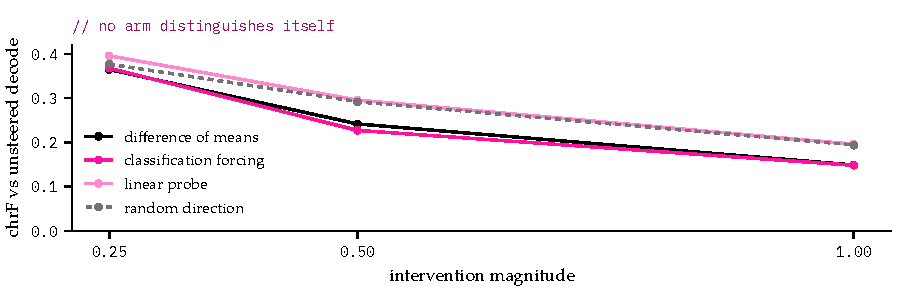
\includegraphics[width=\linewidth]{figures/fig-naturalness.pdf}
\caption{chrF similarity between steered and unsteered decodes as a
function of intervention magnitude. All four arms---including random
perturbations---degrade decoded text at nearly the same rate, with no
method preserving substantially greater similarity at matched magnitude.}
\label{fig:naturalness}
\end{figure}

\paragraph{An entry score as a training objective.} Optimizing a steering
direction on frozen \texttt{resid\_nc\_hm} to maximize a single entry's
quantile-normalized score under a fixed perturbation budget converges
rapidly in the differentiable embedding-space regime, saturating within
roughly 40 gradient-ascent steps (Figure~\ref{fig:rl}). Because gradients
pass directly through the frozen classifier without text decoding, this
regime serves only as an upper bound for decode-cycle optimization---where
rewards pass through discrete text generation and require policy-gradient
estimation such as REINFORCE~\cite{williams1992}---and does not indicate
how quickly REINFORCE would converge. Collateral variation in this setup
is mechanically bounded as well: adding a perturbation of fixed norm $0.5$
to a unit-norm embedding and renormalizing caps angular displacement at
$0.134$, and observed collateral decreases slightly from $0.105$ to
$0.083$ as the learned vector aligns partially with the clean embedding
and reduces its effective post-normalization step. More broadly, additive
output-space perturbations correspond to the residual intervention form
that latent-space steering of diffusion policies improves upon by acting
on the generator's input distribution~\cite{wagenmaker2025}, and
optimizing inputs directly against a frozen classifier can exploit
off-manifold directions along which natural data carry negligible
variance~\cite{makelov2023}. Neither the decode-cycle REINFORCE experiment
nor a sample-efficiency comparison against supervised steering has been
conducted.

\begin{figure}[htbp]\centering
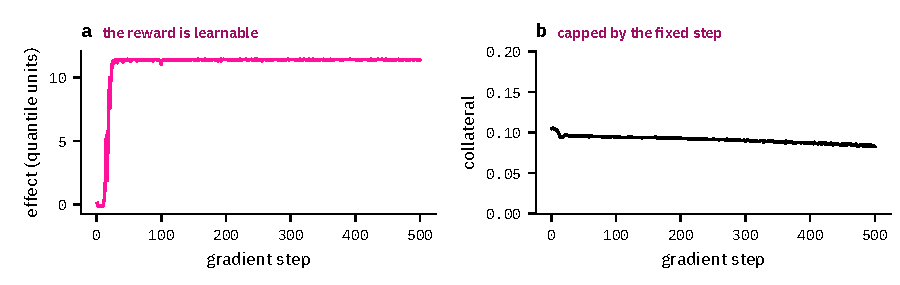
\includegraphics[width=\linewidth]{figures/fig-rl.pdf}
\caption{Optimization of an embedding-space steering vector by gradient
ascent on a single frozen entry's quantile-normalized score in
\texttt{resid\_nc\_hm}. (a) The objective saturates within roughly 40
steps. (b) Collateral displacement---bounded above at $0.134$ by the
fixed perturbation norm---declines from $0.105$ to $0.083$.}
\label{fig:rl}
\end{figure}

\subsection{Head-level autointerp}
\label{sec:headautointerp}

Because single-feature autointerp metrics evaluate individual directions
rather than contrastive partitions, they could in principle understate the
interpretability of classifier heads; we test this hypothesis directly
with a head-level evaluation on \texttt{resid\_nc} at step 372{,}600
(noting the caveat that layer-4 heads in this checkpoint are largely
frozen; Section~\ref{sec:freeze}). Partition descriptions generated from
decoded dictionary parameters alone fail completely, matching the
per-entry result (median accuracy $0.000$, identical to the null).
Activation-grounded head descriptions also fail to outperform a random
null pairing at this sample size (20 heads per condition; median accuracy
$0.083$ vs.\ $0.125$ for the null, where predicting the modal entry alone
scores roughly $0.11$). Furthermore, head-level detection accuracy is
uncorrelated with the mean describability of a head's constituent entries
(Spearman $+0.12$ across 30 head--mode pairs: $+0.25$ with $p{=}0.37$ for
activation descriptions and $+0.05$ with $p{=}0.86$ for parameter
descriptions, 15 heads each). Neither mode yields above-chance head-level
detection, so switching from per-entry to head-level scoring does not
uncover an interpretability advantage in this sample.

\paragraph{Describability and activation density.} Across the six models
in Table~\ref{tab:autointerp}, log nominal activation density correlates
at $-0.894$ with activation-description F1, accounting for roughly 80\% of
the cross-model variance. Fitting a linear regression of
contrastive-description F1 on log empirical firing rate across the four
\texttt{sae.py} runs with nonzero thresholded firing rates (slope
$-0.069$, correlation $-0.766$) while holding out the softmax Ontologizer
predicts an F1 of $0.421$ vs.\ the observed $0.392$ (a residual of $-1.8$
standard errors); thus, the Ontologizer lies close to the empirical
density trend whereas \texttt{g160top1} sits $0.120$ above it. However,
this four-point regression is fragile: the underlying correlation is
modest, \texttt{g160softmax} is excluded because its firing rate above the
$2/k$ threshold is identically zero, and that fixed threshold does not
vary monotonically with effective activation density.

\paragraph{Describability and language concentration.} Tabulating the
number of distinct languages represented among each feature's 15 evaluated
rows (\texttt{autointerp.py language}; Table~\ref{tab:autointerp-lang})
separates the sparse models from the dense ones before any text
description is generated. Within every sparse model, detection F1 declines
sharply as a feature spans more languages (Spearman $-0.47$ to $-0.67$ for
activation descriptions), whereas within the dense models it shows no
trend ($-0.06$ to $+0.03$). In \texttt{k32} and \texttt{g160top1}, a
feature's modal language accounts for $28$--$30\%$ of the held-out
positive examples evaluated by the judge, compared to roughly $1\%$ of the
negative examples and contrastive background draws. Restricting the
log-firing-rate regression of contrastive F1 to multilingual features
spanning 13--15 languages reduces \texttt{g160top1}'s residual above the
trend from $+0.120$ to $+0.018$ and shifts the softmax Ontologizer from
$0.029$ below the trend to $+0.049$ above it. Across individual features,
modal-language purity explains roughly one fifth of the variance in
detection F1 ($0.20$ for activation descriptions and $0.22$ for
contrastive descriptions), whereas log firing rate explains only
$1$--$4\%$. Controlling for language identity directly requires
language-matched negative and background examples---implemented in
\texttt{autointerp.py match} for both contrastive description generation
(\texttt{describe --mode cacts\_lang}) and detection scoring
(\texttt{score --negatives lang})---which have not yet been evaluated.

\begin{table}[htbp]\centering\small\setlength{\tabcolsep}{4pt}
\begin{tabular}{@{}lrrrrrrr@{}}
\toprule
& \multicolumn{4}{c}{features by languages spanned} & & \multicolumn{2}{c}{F1, all / 13--15 languages} \\
\cmidrule(lr){2-5}\cmidrule(l){7-8}
model & 1--3 & 4--9 & 10--12 & 13--15 & purity & \texttt{acts} & \texttt{cacts} \\
\midrule
onto (resid\_nc)   & 0  & 5  & 43 & 177 & 0.158 & 0.473 / 0.460 & 0.392 / 0.380 \\
k32                & 63 & 55 & 68 & 64  & 0.466 & 0.645 / 0.564 & 0.603 / 0.482 \\
k32\_bl            & 9  & 9  & 10 & 47  & 0.277 & 0.578 / 0.502 & 0.470 / 0.338 \\
g160top1           & 41 & 24 & 32 & 53  & 0.440 & 0.646 / 0.467 & 0.594 / 0.383 \\
g160softmax        & 0  & 5  & 72 & 179 & 0.183 & 0.449 / 0.443 & 0.364 / 0.347 \\
k5120 (dense ctrl) & 0  & 2  & 18 & 236 & 0.131 & 0.470 / 0.470 & 0.332 / 0.322 \\
\bottomrule
\end{tabular}
\caption{Detection F1 from Table~\ref{tab:autointerp} stratified by the
number of distinct languages among each feature's 15 evaluated rows (the
10 examples from which each description was generated and the 5 held-out
positives; 15 random rows span an average of $13.8$ languages). Purity is
the fraction of the 10 description rows belonging to their modal language.
One seed per run.}
\label{tab:autointerp-lang}
\end{table}

\section{Supplementary results: the straight-through arm}
\label{app:ste}

\subsection{Calibration}
\label{sec:calib}

A naive port of the live softmax configuration (\texttt{select="ste"})
trains without numerical failure, but the classifier fails to learn. The
root cause is that \textbf{the argmax forward pass is scale-invariant, so
nothing in the uncalibrated configuration drives the logits upward}: they
remain near their initialization scale throughout training (within-head
standard deviation $0.0015$, close to the $2/(d{+}1) \approx 0.0020$ scale
produced by fan-in initialization for a bilinear logit evaluated on a
unit-norm shape vector with its constant coordinate, by the degree-two
analog of the variance argument for scaled dot-product
attention~\cite[fn.~4]{vaswani2017}). VQ-VAE encounters the same
issue---an encoder scale that the discrete code does not constrain---and
addresses it with a commitment loss~\cite{vandenoord2017}. Three
hyperparameter adjustments follow from this scale invariance. First,
\emph{logit noise must be relative}: an absolute scale of
$\sigma_K{=}0.02$ is thirteen times the initial logit spread, causing
noise to dominate the argmax, whereas $\sigma_K{=}0$ eliminates
exploration and causes the codebook to collapse; setting \texttt{--noise-k
batchnorm} (Eq.~\eqref{eq:noise_batchnorm}) scales the noise by the
logit RMS. Second, \emph{the surrogate temperature must match the logit
scale}: at the softmax configuration's floor of $t{=}0.03$, the ratio
spread$/t$ is $0.05$ and the softmax surrogate is nearly flat, so training
reduces to adapting the dictionary to a fixed random partition. Third,
\emph{the batch-mean uniformity weight $s_{\mathrm{KL}_m}$ must be
rescaled}: the softmax default of $10^{-6}$ is calibrated against a
whitened MSE near $3\times10^{-6}$, whereas a hard code trains at an MSE
orders of magnitude larger, rendering a $10^{-6}$ weight effectively inert
and allowing heads to collapse. A 4{,}000-step sweep over the surrogate
temperature $t$ (learning rate $10^{-5}$, \texttt{--noise-k batchnorm
--sd-k 0.3}; one seed per arm, which suffices to rank configurations
though not to predict final converged error) illustrates the trade-off:

\begin{center}\small
\begin{tabular}{@{}lrrrr@{}}
\toprule
$t$ & spread$/t$ & max $p$ & effective entries/head & raw FVU \\
\midrule
0.01    & 0.15  & 0.043 & 23.4 & 178 \\
0.0015  & 0.78  & 0.135 & 26.4 & 193 \\
0.0005  & 3.38  & 0.681 & 14.0 & 59.2 \\
0.00015 & 16.84 & 0.974 & 3.8  & 7.3 \\
\bottomrule
\end{tabular}
\end{center}

Sharpening the surrogate enables the classifier to train and reduces raw
FVU 25-fold, but it trades off directly against entry utilization, which
must be maintained by $s_{\mathrm{KL}_m}$. At \texttt{sonar.py}'s default
learning rate of $5\times10^{-5}$, every sharp-surrogate arm collapsed
abruptly after roughly 1{,}700 steps, whereas $10^{-5}$ remains stable.
The shipped SONAR arm therefore uses $t{=}1.5\times10^{-4}$, a learning
rate of $10^{-5}$, \texttt{--noise-k batchnorm --sd-k 0.3}, and
$s_{\mathrm{KL}_m}{=}10^{-4}$, trained for 24 epochs (369{,}500 steps).
Because $t$ is manually matched to a single initial logit-scale
measurement, however, effective sharpness drifts as the logit scale
evolves: over training, the shipped arm's layer-0 logits shrink 2.9-fold,
reducing spread$/t$ from $13$ at initialization to $4.5$, while relative
batchnorm noise flips 20--29\% of layer-0 assignments throughout
(\texttt{logitscale.py}, evaluated on 2{,}048 tail rows). More generally,
scale invariance leaves the logits free to drift in either direction, and
the GPT-2 arms---trained at the naive port's uncalibrated
settings---exhibit the opposite drift. In GPT-2 \texttt{ste\_h76}, whose
classifier lacks a gate, layer-0 logits grew 452-fold; consequently, its
fixed-scale absolute noise flipped more than half of layer-0 assignments
through 50{,}000 steps, but only about 1\% from 150{,}000 steps onward. By
contrast, the sigmoid-gated classifiers in the concatenated GPT-2 seed
pair remained near their initial scale, so the same absolute noise flipped
71--90\% of layer-0 assignments across all 16 evaluated checkpoints. A
more principled calibration would either normalize logits per head or
adapt $t$ online to maintain a target spread$/t$ setpoint.

\subsection{Capacity beyond bits, and training dynamics}
\label{sec:capacity}

\paragraph{Distance from the Gaussian reference.} Evaluated relative to
the Gaussian rate--distortion reference at each code's bit rate, the full
five-layer stack lies further above the bound than a single-layer prefix.
Because the optimal distortion achievable on non-Gaussian embeddings can
only lie at or below the Gaussian reference for a covariance-matched
source, each ratio lower-bounds the code's suboptimality at its rate:

\begin{center}\small
\begin{tabular}{@{}lrrr@{}}
\toprule
code & Gaussian reference & achieved & ratio \\
\midrule
380 bits (one layer's prefix) & 0.4208 & 0.537 & 1.28$\times$ \\
1900 bits, $5\times76$ & 0.0499 & 0.1535 & 3.08$\times$ \\
1900 bits, $5\times380$, $k{=}2$ & 0.0499 & 0.1844 & 3.70$\times$ \\
\bottomrule
\end{tabular}
\end{center}

\paragraph{Bits are not the whole capacity.} At an identical 1900-bit
budget, a $5\times380$ stack of binary heads ($k{=}2$) reaches $\fvu =
0.1844$, compared to $\fvu = 0.1535$ for the $5\times76$ stack of 32-way
heads: whereas bit rate scales as $h\log_2 k$, total codebook size scales
as $h\cdot k$ (3{,}800 vs.\ 12{,}160 atoms across five layers). Because
the binary arm was also trained at half the batch size
(Table~\ref{tab:cfg-ste-sonar}), this gap reflects both the smaller
codebook and higher gradient variance. Residual vector quantizers in
neural audio codecs exhibit the same trade-off: at a fixed 80 bits per
frame, eight stages of 1{,}024 codes outperform eighty binary
stages~\cite{zeghidour2021}. Even so, the binary arm comes within 17\% of
the 32-way stack using $2.9\times$ fewer parameters while representing
each head as a single binary feature---a format directly amenable to
naming.

\paragraph{Realized bits, and what they bound.} Following standard
information-theoretic convention, this paragraph denotes random variables
in uppercase. For a deterministic hard code evaluated on a random input
$\mathbf{X}$, let $A_{\ell i}$ denote the entry selected by head
$(\ell,i)$ and let $\mathbf{A}$ denote the joint assignment across all
heads. The \emph{realized bits} are defined as the sum of marginal usage
entropies across heads,
\begin{equation}
	H_{\mathrm{real}} := \sum_{\ell,i} H(A_{\ell i})
	= \sum_{\ell,i} \big(\log_2 k - \mathrm{KL}(\bar{\mathbf{p}}_{\ell i} \,\Vert\, \mathrm{uniform})\big)
	\;\geq\; H(\mathbf{A}) = I(\mathbf{X}; \mathbf{A}),
	\label{eq:realized}
\end{equation}
where $\bar{\mathbf{p}}_{\ell i}$ is the marginal usage distribution (mean
assignment) of head $(\ell,i)$; in terms of the logged statistic
$\mathrm{KL}_m$ summed over layers, this equals
$h(l\log_2 k - \mathrm{KL}_m)$. Because $\mathbf{A}$ is a deterministic
function of $\mathbf{X}$, its joint entropy $H(\mathbf{A})$ equals the
mutual information $I(\mathbf{X}; \mathbf{A})$, which is upper-bounded by
$H_{\mathrm{real}}$ by subadditivity, with equality if and only if all
heads are mutually independent. Consequently, $H_{\mathrm{real}}$ measures
per-head entry uniformity rather than true information content: two codes
with identical $H_{\mathrm{real}}$ can carry different amounts of
information depending on inter-head redundancy, and we do not estimate the
joint entropy $H(\mathbf{A})$, which would require density estimation over
$k^{lh}$ outcomes.

\paragraph{Training dynamics.} In the shipped arm, the logged training MSE
(averaged across deep-supervision prefixes) plateaus from step 237k
onward, whereas within-head row collinearity continues to fall ($0.812 \to
0.686$, compared to ${\sim}0.64$ for random non-negative atoms). Entry
usage in the shipped arm collapses early in training and never becomes
fully uniform (Figure~\ref{fig:realized-bits}): realized bits drop to 43\%
of the nominal 1900 bits near step 6k, recover to 85\% by step 20k as the
rescaled $s_{\mathrm{KL}_m}$ penalty counteracts collapse, and finish at
90\%. Under the fixed initialization, by contrast, every head reaches
near-uniform usage by step 5k (99\% of nominal) in both the five-layer
stack and the flat arm, and remains there throughout training. We compute
realized bits from the logged $\mathrm{KL}_m$ as
$h(l\log_2 k - \mathrm{KL}_m)$ minus its finite-sample floor: because
$\mathrm{KL}_m$ is a plug-in estimate on a single batch of $b{=}256$ rows,
even perfectly uniform usage yields an expected floor of
$(k-1)/(2b\ln 2) = 0.087$ bits per layer, which accounts for nearly the
entire logged value in the converged fixed-initialization arms. After this
correction, the final values match the held-out measurements in
Table~\ref{tab:init} to within 1 bit on the fixed-initialization arms,
while overstating the shipped arm by 14 bits because the correction
assumes that all $k$ entries remain live.

\begin{figure}[tp]\centering
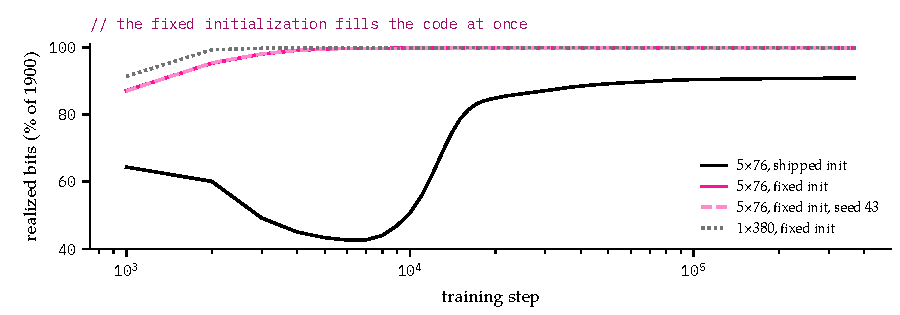
\includegraphics[width=\linewidth]{figures/fig-realized-bits.pdf}
\caption{Realized code bits over training as a fraction of the nominal
1900 bits, computed from the logged $\mathrm{KL}_m$ minus its single-batch
sampling floor. Under the shipped initialization, entry usage drops below
half of nominal capacity before recovering to 90\% (the plotted 91\%
slightly over-corrects heads with dead entries); under the fixed
initialization, every head in both the five-layer stack and the flat arm
reaches near-uniform usage within 5k steps. Realized bits upper-bound the
information carried by the code rather than measuring it directly
(Eq.~\eqref{eq:realized}).}
\label{fig:realized-bits}
\end{figure}

\subsection{Operational rate: every code quantized}
\label{sec:quantrate}

Comparing raw index bits and active coefficient counts cannot directly
rank codes that transmit continuous magnitudes against purely discrete
codes. Quantizing and entropy-coding all transmitted values
(Eq.~\eqref{eq:quantrate}) places every model on a common operational
rate--distortion axis (Figure~\ref{fig:quantrate}). Evaluating each code
at the five-layer stack's 1900-bit budget yields the following held-out
$\fvu$:

\begin{center}\small\setlength{\tabcolsep}{4pt}
\begin{tabular}{@{}lrrrr@{}}
\toprule
code & \stackhead[r]{$\fvu$\\unquantized} & \stackhead[r]{1900 bits,\\entropy-coded} & \stackhead[r]{1900 bits,\\fixed supports} & \stackhead[r]{1900 bits\\on every row} \\
\midrule
straight-through, $5\times76$ & 0.1536 & \textbf{0.155} & \textbf{0.158} & 0.158 \\
L1 SAE, $s_{\mathrm{L1}}{=}3\times10^{-6}$ & 0.0052 & \textbf{0.129} & 0.182 & \textbf{0.152} \\
softmax Ontologizer & 0.0054 & 0.145 & 0.239 & --- \\
L1 SAE, $s_{\mathrm{L1}}{=}10^{-5}$ & 0.048 & 0.175 & 0.180 & 0.200 \\
L1 SAE, $s_{\mathrm{L1}}{=}3\times10^{-5}$ & 0.219 & 0.242 & 0.243 & 0.250 \\
$\topk$ SAE, $k_{\mathrm{SAE}}{=}5120$ & 0.0001 & 0.243 & --- & 0.281 \\
$\topk$ SAE, $k_{\mathrm{SAE}}{=}160$ & 0.258 & 0.259 & 0.259 & 0.258 \\
\texttt{g160top1} & 0.274 & 0.274 & 0.274 & 0.274 \\
\texttt{g160softmax} & 0.0044 & 0.372 & 0.364 & 0.454 \\
\bottomrule
\end{tabular}
\end{center}

Under per-slot entropy coding at an average rate of 1900 bits per row, a
coarsely quantized ReLU+L1 SAE ($s_{\mathrm{L1}}{=}3\times10^{-6}$)
outperforms the hard stack ($\fvu = 0.129$ vs.\ $0.155$), and matches the
stack's gain-pinned discrete error of $0.158$ at 1{,}675 bits. Near 1900
bits, this L1 SAE transmits roughly 440 of its ${\sim}1{,}600$ active
coefficients at about 4.3 bits per coefficient including support indexing.
Because L1 latents fire with skewed frequencies, entropy coding compresses
its support indices to roughly 20\% below their fixed-length combinatorial
cost, whereas the hard stack uses entries almost uniformly (1895 of 1900
bits; Table~\ref{tab:init}) and therefore saves almost nothing under
entropy coding. At the same time, the L1 SAE's code length varies
substantially across inputs: near a 1900-bit average rate, per-row bit
lengths span 1{,}406 to 2{,}399 bits (5th to 95th percentile). By
contrast, the hard stack's gain-pinned discrete code uses exactly 1900
bits on every row at fixed length, and under entropy coding its per-row
lengths differ only by the few bits induced by minor entry-frequency
variations. When we enforce a strict 1900-bit budget on every row---choosing
for each row the finest quantization step that fits after reserving
roughly 6 bits to specify the step---the $s_{\mathrm{L1}}{=}3\times10^{-6}$
SAE reaches $\fvu = 0.152$, nearly tied with the stack, and requires
1{,}853 bits per row to match the stack's $0.158$. Fixed-support codes do
not change under per-row capping, whereas other variable-rate codes lose
ground (from $0.243$ to $0.281$ for the dense $k_{\mathrm{SAE}}{=}5120$
SAE and from $0.372$ to $0.454$ for \texttt{g160softmax}). Whereas average
rate is the standard metric for corpus compression, a per-row budget
provides a fairer comparison for a fixed-size per-input representation.
When supports are charged their fixed-length combinatorial cost, the hard
stack outperforms every SAE ($0.158$ vs.\ $0.180$).

Among fixed-sparsity baselines, the $k_{\mathrm{SAE}}{=}160$ $\topk$ SAE
plateaus at its unquantized error from roughly 1900 bits onward---consistent
with its unquantized least-squares support floor of $0.236$---and already
reaches $\fvu = 0.275$ at 1{,}121 bits, indicating that its coefficients
convey little beyond support identity; the single-layer hard variant
\texttt{g160top1} behaves similarly. Quantizing the softmax Ontologizer's
assignments around their mean reaches $\fvu = 0.145$ at 1900 average bits,
with the same value on freshly encoded out-of-sample rows held out from
all models. In the hard stack, quantizing the four scalar gains requires 4.8
bits at a step size of two standard deviations (reducing $\fvu$ from
$0.158$ to $0.155$) and 28 bits to recover the unquantized $\fvu$ of
$0.1536$. Finally, none of these checkpoints were trained for an
entropy-coded quantization pipeline: uniform usage is the worst case for
entropy coding, and none of the SAEs were trained with quantized
coefficients, so these curves rank the trained models rather than the
architectures themselves.

\paragraph{On the sentence cache.}
In the recipe-ladder sweep (\texttt{experiments/\allowbreak recipe-ladder}), we
trained both the $5\times76$ hard stack ($k{=}32$) and a $5\times54$
direct-atom stack ($k{=}128$, signed atoms) on \texttt{mc4\_sent16} for
50{,}000 steps each with all four auxiliary loss weights disabled
(\texttt{--s-bcossim 0 --s-support 0 --s-l1f 0 --s-hm 0}). Evaluating both
stacks alongside SAEs trained on the same cache at a 1900-bit budget
yields:

\begin{center}\small\setlength{\tabcolsep}{4pt}
\begin{tabular}{@{}lrrrr@{}}
\toprule
code & \stackhead[r]{$\fvu$\\unquantized} & \stackhead[r]{averaged\\over rows} & \stackhead[r]{on every\\row} & \stackhead[r]{one step\\every row fits} \\
\midrule
direct-atom stack & 0.1611 & 0.161 & 0.164 & \textbf{0.164} \\
hard stack & 0.1681 & 0.172 & 0.189 & 0.189 \\
$\topk$ SAE, $k_{\mathrm{SAE}}{=}256$ & 0.1260 & \textbf{0.128} & \textbf{0.129} & 0.185 \\
L1 SAE, $s_{\mathrm{L1}}{=}4.64\times10^{-7}$ & 0.0526 & 0.142 & 0.174 & 0.499 \\
$\topk$ SAE, $k_{\mathrm{SAE}}{=}160$ & 0.1872 & 0.187 & 0.187 & 0.188 \\
\bottomrule
\end{tabular}
\end{center}

\noindent A wider $\topk$ SAE ($k_{\mathrm{SAE}}{=}256$ active out of
11{,}264 latents) outperforms both stacks both at 1900 average bits and
under a 1900-bit per-row cap using per-row step selection. Because its
per-row code lengths vary much less than those of the L1 SAE (1{,}734 to
2{,}133 bits from the 5th to 95th percentile, vs.\ 974 to 3{,}359 bits),
imposing a per-row budget penalizes it very little. The hard stacks lead
only when a single global quantization step must fit every row, which
penalizes a code according to its longest row: under that constraint, the
$k_{\mathrm{SAE}}{=}256$ SAE averages only 1{,}107 bits per row, leaving
roughly 800 bits unused. By contrast, the $k_{\mathrm{SAE}}{=}160$ SAE
trails the direct-atom stack under every accounting, and trails the
$5\times76$ hard stack at average rate ($0.187$ vs.\ $0.172$) while
roughly matching it under strict per-row caps ($0.187$--$0.188$ vs.\
$0.189$). Each code is evaluated from a single training seed.

\begin{figure}[tp]\centering
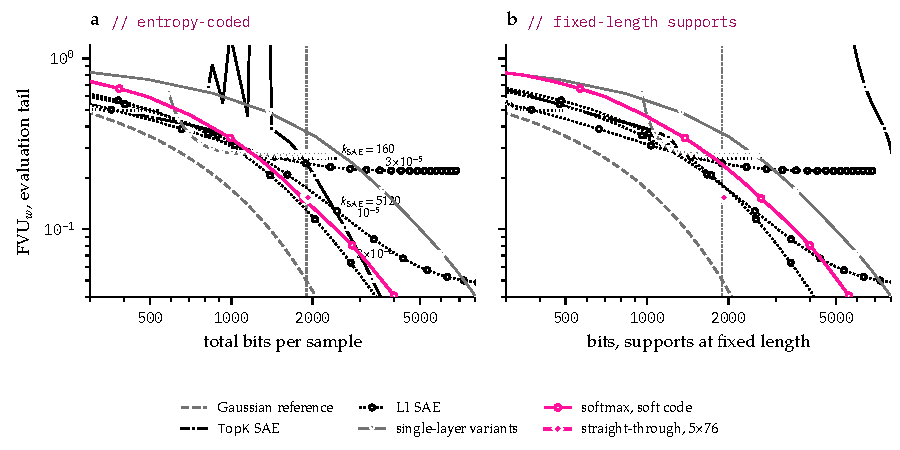
\includegraphics[width=\linewidth]{figures/fig-quantrate.pdf}
\caption{Operational rate--distortion curves on the evaluation tail with
all transmitted values quantized across a sweep of step sizes
(Eq.~\eqref{eq:quantrate}): (a) per-slot entropy coding of all symbols,
and (b) fixed-length combinatorial support costs with entropy-coded
nonzero values. ReLU+L1 SAEs are labeled by $s_{\mathrm{L1}}$; the
unlabeled $\topk$ curve is $k_{\mathrm{SAE}}{=}32$, and the single-layer
variants are \texttt{g160top1} (flat) and \texttt{g160softmax}
(downward-sloping). The straight-through stack spans 1895--1923 bits. The
vertical dotted line marks 1900 bits and the dashed curve shows the
Gaussian rate--distortion reference (Eq.~\eqref{eq:ratefloor}). Although
the softmax Ontologizer included the evaluation tail during training,
re-evaluating on freshly encoded rows held out from all models changes
every curve's $\fvu$ at 1900 bits by at most $0.0004$
(Appendix~\ref{app:data}).
Each curve represents a single seed.}
\label{fig:quantrate}
\end{figure}

\subsection{Depth: eliminations and mechanism}
\label{sec:depthdetail}

\paragraph{Over training.} Evaluated on the held-out tail every 10k steps
(Figure~\ref{fig:depth-curves}), the five-layer stack outperforms the
flat arms from the first checkpoint onward: the error ratio relative to
the matched flat arm is $1.59\times$ at step 10k, peaks at $1.83\times$
near step 200k, and finishes at $1.79\times$. Neither architecture has
fully converged. Over the final quarter of training, $\fvu$ improves by
$0.86\%$ in the stack and by $2.3$--$2.75\%$ in the flat arms, indicating
that the gap narrows slowly and that longer runs would be required to
determine its asymptote. Seed replicas overlap closely at every
checkpoint.

\begin{figure}[tp]\centering
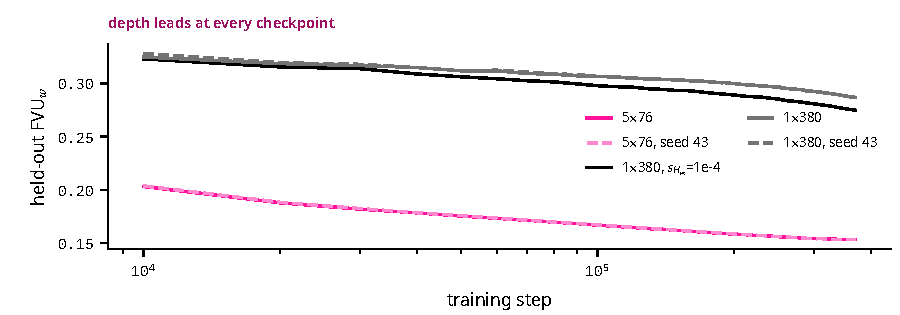
\includegraphics[width=\linewidth]{figures/fig-depth-curves.pdf}
\caption{Held-out $\fvu$ over training for the $5\times76$ stack and the
$1\times380$ flat arms at matched bit budget and parameter count, with
seed replicas. The flat arm trained with the stack's batch-mean
uniformity weight ($s_{\mathrm{KL}_m}{=}10^{-4}$) is the configuration
compared in Section~\ref{sec:depth}.}
\label{fig:depth-curves}
\end{figure}

Two earlier, confounded versions of this comparison under the shipped
initialization help isolate what residual depth contributes. First, an
unadjusted flat arm reached $\fvu = 0.5822$ at 484 realized bits (25.5\%
of nominal), a $2.5\times$ gap relative to the shipped stack. Because
$\mathrm{KL}_m$ averages across a layer's $h$ heads before summing across
layers, per-head uniformity pressure from $\mathrm{KL}_m$ scales as
$s_{\mathrm{KL}_m}/h$ per layer, meaning that the $1\times380$ flat arm
had trained under one fifth of the per-head uniformity pressure of the
$5\times76$ stack; matching per-head uniformity pressure raised realized
usage to 1{,}199 bits and reduced $\fvu$ to $0.4307$. Second, inserting a
frozen ZCA whitener (\texttt{make\_zca.py}) before the flat classifier
increased the input's effective dimension from 107 to 901 and drove usage
to 1{,}900 of 1{,}900 bits (4.999 of 5 bits per head, exceeding the
shipped stack's own utilization), yet reconstruction remained $1.7\times$
worse than the stack ($\fvu = 0.3842$). Two conclusions survive from
these ablations. First, \textbf{entry utilization does not explain the
benefit of depth}---nor does maximizing realized bits optimize
distortion, since reducing $s_{\mathrm{KL}_m}$ by $100\times$ in the
shipped stack costs 176 realized bits while \emph{improving} $\fvu$ to
$0.2095$. Second, \textbf{a jointly learned input transform collapses
where a frozen whitener succeeds}: prepending a trainable \texttt{Linear}
encoder causes every head to collapse onto exactly two entries at $\fvu =
0.6853$, performing worse than no encoder at all.

\paragraph{The input each classifier receives.} Measuring the geometry of
the exact input vector passed to each layer's classifier in the shipped
arm (\texttt{inputgeom.py}) reveals a sharp conditioning transition after
layer 0:

\begin{center}\small
\begin{tabular}{@{}lrrr@{}}
\toprule
layer & mean direction & mean pairwise cos & effective dim / 1024 \\
\midrule
0 & 0.5638 & 0.3146 & 107.5 \\
1 & 0.0932 & 0.0087 & 611.3 \\
2 & 0.1522 & 0.0233 & 596.3 \\
3 & 0.1983 & 0.0396 & 548.8 \\
4 & 0.2348 & 0.0553 & 507.1 \\
\bottomrule
\end{tabular}
\end{center}

Layer 0 (like every single-layer flat arm) classifies raw embeddings
concentrated in a narrow spherical cap, whereas layers 1--4 classify
residuals whose effective dimension spans more than half of the
1024-dimensional space. In the shipped arm, layer 0 was the only layer
whose heads left most entries unused (10.6 live entries and 216 realized
bits, compared to ${\sim}375$ bits in each deeper layer), providing a
within-model control that holds architecture and hyperparameters fixed
while varying only the input distribution.

\paragraph{What the cascade contributes: pairing.}
Without retraining, \texttt{blendablate.py} interpolates the subtracted
term $\mathrm{dec}(\mathbf{r}_\ell)$ in layer $\ell$'s input toward a
reference distribution with matched marginals but no sample-level
pairing---another row's reconstruction (shuffle), the corpus mean, or
Gaussian noise rescaled to match the shuffled reconstruction's per-sample
magnitude:

\begin{center}\small
\begin{tabular}{@{}lrrrrr@{}}
\toprule
blend & shuffle & mean & noise & eff.\ dim L1 (shuffle) & (noise) \\
\midrule
0.000 & 0.2292 & 0.2292 & 0.2292 & 499.1 & 499.1 \\
0.125 & 0.2460 & 0.2374 & 0.2426 & 476.0 & 504.7 \\
0.250 & 0.3084 & 0.2652 & 0.2838 & 394.2 & 518.3 \\
0.500 & 0.6910 & 0.4100 & 0.4665 & 193.4 & 539.6 \\
0.750 & 1.8154 & 0.7497 & 0.8502 & 103.0 & 527.6 \\
1.000 & 4.6613 & 1.4302 & 1.5992 & 68.5 & 496.2 \\
\bottomrule
\end{tabular}
\end{center}

Sample-specific pairing is critical well before the residual link is
completely severed: a 0.25 blend increases $\fvu$ by 35\%, and
substituting another row's reconstruction degrades reconstruction more
than magnitude-matched Gaussian noise at every blend level, showing that
the degradation reflects lost pairing rather than generic perturbation
sensitivity. This sweep cannot, however, separate pairing from
conditioning: effective dimension drops in lockstep with rising error
because a residual is small and nearly isotropic precisely when it
subtracts the sample's own coarse reconstruction. That observation
reconciles this ablation with the ZCA-whitened flat arm: whitening
provides isotropic conditioning without residual pairing, yielding uniform
entry usage while improving $\fvu$ by only ${\sim}7\%$. (Training with
\texttt{forward="labels"}, which would test this directly by removing the
residual stream altogether, has not been run under the fixed
initialization. Forwarding upstream assignments \emph{alongside} the
residual via \texttt{forward="resid\_labels"} performed poorly in a
three-epoch pilot, finishing at held-out $\fvu = 0.826$ vs.\ $0.249$
despite leading by $50\times$ early in training; because the residual by
construction isolates what upstream codes failed to explain, appending
those codes adds parameters without adding information.)

\paragraph{The code is not the whole channel.} Each layer decomposes its
input into a unit direction---which is all that the classifier
receives---and a scalar L2 norm (gain) that multiplies the layer's output,
allowing one continuous scalar per layer per sample to reach the decoder
outside the discrete bottleneck. Pinning each gain to its held-out mean
(\texttt{gainablate.py}) increases the stack's $\fvu$ by $+3.0\%$ in
total, or $+0.6\%$ to $+0.8\%$ per active layer (layer 0's gain is
identically $1$ because the cached embeddings are L2-normalized, whereas
raw SONAR embeddings are not~\cite{sonar}), compared to the 79\% margin
by which the matched flat arm trails the stack. Thus, while the continuous
gain channel is real, it does not explain the advantage of depth. With
its gains pinned, the stack becomes a purely discrete 1900-bit code
($\fvu = 0.158$), which is the variant compared against SAEs at matched
total rate in Section~\ref{sec:ste}. The gain channel is, however, a
nontrivial confound for the ZCA-whitened flat arm, where whitening
introduces a varying layer-0 gain whose pinning costs $+4.5\%$ in
$\fvu$, accounting for roughly 40\% of whitening's apparent benefit.

\paragraph{The decoder is dense, and not because of the offset.}
Magnitude-pruning the smallest half of the trained decoder's weights
drives $\fvu$ into the thousands, and its weight distribution closely
resembles that of a dense Gaussian matrix. Because dictionary atoms are
non-negative, the accumulator's mean vector dwarfs its sample-to-sample
variation ($\lVert\mathbb{E}\mathbf{r}\rVert / \mathbb{E}\lVert
\mathbf{r}-\mathbb{E}\mathbf{r}\rVert = 11.6$), and the bias-free decoder
attenuates that constant component to match the corpus embedding mean
(norm $0.581$ vs.\ $0.564$). Adding an explicit decoder bias
(\texttt{--biased-dec}), however, changes training MSE by only $-0.62\%$
at a matched step (that run terminated early at 23\% of its schedule, so
its held-out $\fvu = 0.2464$ is not comparable to the converged arm):
fixing $W_{\mathrm{dec}}\,\mathbb{E}\mathbf{r}$ imposes 1{,}024 linear
constraints on a $1024\times2048$ matrix, or $0.05\%$ of its degrees of
freedom. The decoder is dense simply because transporting an
approximately 900-dimensional signal requires a dense full-rank linear
map.

\paragraph{How the layers' partitions relate.} Each head's winning entry
partitions the evaluation tail, and Figure~\ref{fig:headnmi} compares all
pairs among the 380 heads of \texttt{ste\_h76} under the shipped
initialization (\texttt{headnmi.py}). Heads partition the inputs nearly
independently except within layer 0: mean chance-adjusted NMI within a
layer is $0.0075$ at layer 0 and $0.0006$--$0.0028$ in layers 1--4, and
at most $0.0004$ between layers (in the GPT-2 stack, $0.054$ at layer 0
and at most $0.004$ elsewhere), indicating that deeper layers do not
redundantly subdivide partitions created by earlier layers. Causal
coupling---measured by effective information, or how much forcing one head
shifts another head's assignment distribution---tracks partition overlap
only when intervening at layer 0: across head pairs, its Spearman
correlation with adjusted NMI is $0.76$, $0.50$, $0.38$, and $0.23$ from
layer 0 into layers 1--4, respectively, and at most $0.08$ from any
deeper layer, whose heads shift every downstream head by a comparable
$0.003$--$0.02$ bits regardless of partition overlap. Results are reported
for a single seed.

\begin{figure}[tp]
\centering
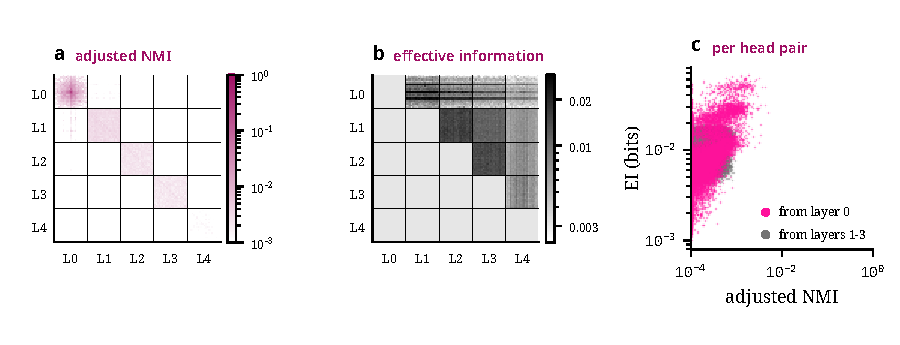
\includegraphics[width=\linewidth]{figures/fig-headnmi.pdf}
\caption[Head partitions against each other and against
intervention]{\textbf{Partitions overlap and track causal coupling only
	from layer 0.} Evaluation of the 380 heads of \texttt{ste\_h76}
	(shipped initialization) on the evaluation tail, grouped by layer and
	ordered within each layer by hierarchical clustering. (a)
	Chance-adjusted NMI between all pairs of heads' winning-entry
	partitions ($0 = \text{chance}$, log scale; diagonal shaded gray). (b)
	Effective information from the row head to the column head under
	uniform interventions over the source head's live entries
	(non-downstream pairs shaded gray). (c) Effective information vs.\
	adjusted NMI per head pair, stratified by source layer. Evaluated on
	a single seed.}
\label{fig:headnmi}
\end{figure}

\subsection{Steering by target layer, and head-health levers}
\label{sec:steerlayer}

Stratifying the five-layer stack's steering realization rate by target
layer (at step strength $1.0$, across 12 entries per layer) reverses the
aggregate ranking of steering directions:

\begin{center}\small
\begin{tabular}{@{}lrrrrr@{}}
\toprule
layer & decode & grad & margin & adjoint & random \\
\midrule
0 & 0.216 & \textbf{0.583} & 0.547 & 0.237 & 0.034 \\
1 & 0.464 & 0.089 & 0.367 & 0.000 & 0.023 \\
2 & 0.742 & 0.130 & 0.216 & 0.000 & 0.055 \\
3 & \textbf{0.966} & 0.130 & 0.091 & 0.000 & 0.034 \\
4 & 0.362 & 0.047 & 0.036 & 0.005 & 0.047 \\
\bottomrule
\end{tabular}
\end{center}

At layer 0, where the input perturbation reaches the classifier directly,
directions derived from the classifier's own geometry (\texttt{grad} and
\texttt{margin}) outperform \texttt{decode} three- to tenfold. At deeper
layers, however, classifier-local directions fail: a gradient computed
with respect to layer $\ell$'s residual input is valid only locally, and
an input-space perturbation arrives at layer $\ell$ only after earlier
layers have re-encoded and subtracted from it. By contrast, the
\texttt{decode} direction shifts the input toward the vector emitted when
the target entry is active, remaining self-consistent across the residual
cascade. Layer 4 is difficult to steer along any direction because its
residual is nearly exhausted. Practically, layer 0 is best steered via
classifier gradients and layers 1--3 via decoded atoms.

\paragraph{Head-health levers and steering.} We evaluated three training
interventions intended to improve head health and steerability on the
shipped stack. First, \emph{batch-mean uniformity pressure from
$\mathrm{KL}_m$ does not account for reduced steerability}: a twin
trained at $s_{\mathrm{KL}_m}{=}10^{-6}$ achieves a raw text-cycle
steering effect of $0.043$ vs.\ $0.027$, both an order of magnitude below
\texttt{top2} and \texttt{top8} models trained at the same weight. Hard
argmax selection itself, rather than the $\mathrm{KL}_m$ uniformity
penalty, therefore accounts for the loss of steerability, while lowering
$s_{\mathrm{KL}_m}$ substantially degrades entry usage (increasing usage
imbalance from $2.71$ to $5.00$ bits). Second, \emph{head-independence
penalties based on HSIC/CKA optimized finite-sample estimator bias rather
than genuine dependence} (Section~\ref{sec:hsic}). Third, \emph{a
row-collinearity setpoint substantially improves steerability}: capping
within-head atom cosine at $0.5$ (compared to $0.774$ in the uncontrolled
run) increases embedding-space realization across every steering direction
(\texttt{decode} $+15\%$, \texttt{grad} $+17\%$, \texttt{margin} $+52\%$,
and oriented \texttt{adjoint} $+122\%$) while reducing collateral
($0.591 \to 0.552$) and slightly improving held-out $\fvu$ ($0.2157$ vs.\
$0.2293$). The setpoint controller acts only transiently during early
training (Figure~\ref{fig:kcos}): as the maximum within-head atom cosine
across heads and layers climbs past $0.8$, the multiplier
$s_{\mathrm{kcossim}}$ rises to $4.9\times10^{-3}$ near step 35k and
drives the statistic down to the $0.5$ setpoint by step 50k; from roughly
step 60k onward, the multiplier projects to zero and the maximum cosine
remains at or below $0.5$ without further penalty, finishing at $0.473$
vs.\ $0.774$ in the uncontrolled run. Why this early transient improves
steerability remains unexplained: the controlled statistic is evaluated in
the $e$-dimensional dictionary space, where 74--78\% of each atom's
energy lies in the decoder's null space (Section~\ref{sec:rowcos}), and
the decoded atoms were already nearly orthogonal. That the
classifier-derived directions exhibit the largest gains suggests an
indirect effect on classifier training rather than on the decoded
dictionary, though nothing establishes this mechanism directly. Finally,
the setpoint provides no benefit on the single-layer flat arm, where
realization is already saturated ($0.992$ vs.\ $0.966$).

\begin{figure}[tp]\centering
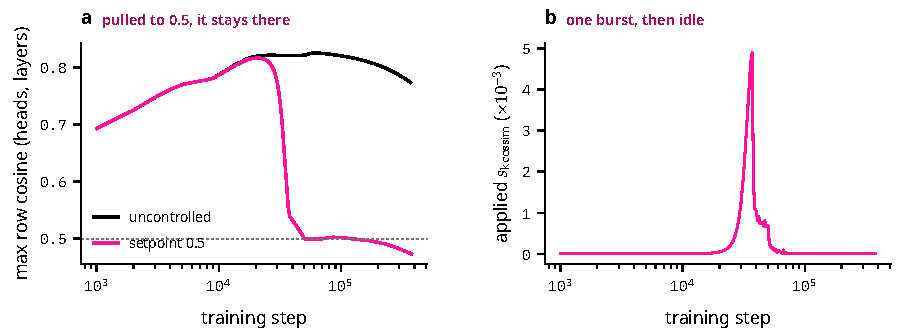
\includegraphics[width=\linewidth]{figures/fig-kcos.pdf}
\caption{Row-collinearity setpoint controller dynamics on the shipped
stack, taken from the training log. (a) Maximum within-head row cosine
across heads and layers---the statistic monitored by the
controller---compared to the uncontrolled twin; the dotted line marks the
$0.5$ setpoint. (b) Applied multiplier $s_{\mathrm{kcossim}}$, averaged
over 1{,}000-step windows.}
\label{fig:kcos}
\end{figure}

\subsection{Supervised vectors at their own step size}
\label{sec:steersupnative}

Whereas Table~\ref{tab:steersup} compares steering directions at a fixed
step size, each native intervention also carries a natural step magnitude:
for an Ontologizer, the decoded output change produced by forcing the
target entry; for an SAE latent, its decoder direction scaled by its mean
nonzero activation; and for the difference of means, the unrescaled
mean-difference vector itself, matching the step taken by activation
addition. Evaluating each direction at its native step length yields the
following rates (reported as realized / collateral, followed in
parentheses by the median step norm as a fraction of
$\lVert\mathbf{x}\rVert$, alongside the collateral of a norm-matched
isotropic random step):

\begin{center}\small\setlength{\tabcolsep}{4pt}
\begin{tabular}{@{}lrrr@{}}
\toprule
model & \stackhead[r]{own\\(step)} & \stackhead[r]{diff.\ of means\\(step)}
& \stackhead[r]{random:\\own / dm} \\
\midrule
softmax stack & 0.19 / 0.25 (0.064) & 0.18 / 0.25 (0.079) & 0.25 / 0.30 \\
hard-code stack & 0.08 / 0.54 (0.129) & \textbf{0.27} / 0.47 (0.064) & 0.53 / 0.48 \\
hard-code flat & 0.17 / 0.04 (0.028) & \textbf{0.54} / 0.12 (0.087) & 0.05 / 0.17 \\
untrained stack & 0.00 / 0.00 (0.001) & \textbf{0.53} / 0.17 (0.162) & 0.00 / 0.17 \\
random-projection heads & \textbf{0.67} / 0.28 (0.206) & 0.55 / 0.20 (0.146) & 0.27 / 0.20 \\
\texttt{g160top1} & 0.41 / \textbf{0.01} (0.186) & 0.57 / 0.04 (0.053) & 0.18 / 0.07 \\
\texttt{g160softmax} & 0.54 / 0.07 (0.050) & 0.57 / 0.13 (0.107) & 0.08 / 0.16 \\
$\topk$ SAE, $k_{\mathrm{SAE}}{=}32$ ($m{=}5120$) & 0.46 / 0.06 (0.072) & \textbf{0.77} / 0.15 (0.180) & 0.07 / 0.17 \\
$\topk$ SAE, $k_{\mathrm{SAE}}{=}32$ ($m{=}11264$) & 0.50 / 0.08 (0.076) & \textbf{0.82} / 0.17 (0.172) & 0.09 / 0.19 \\
SAE, bilinear encoder & 0.82 / 0.04 (0.078) & 0.88 / 0.08 (0.121) & 0.04 / 0.07 \\
\bottomrule
\end{tabular}
\end{center}

Across most models, the difference of means achieves higher realization,
though in the SAEs and the flat hard-code arm this comes partly from
taking $2$--$3\times$ larger steps. In the five-layer hard-code stack,
however, direction rather than step length is decisive: the supervised
vector reaches its target entries more than three times as often using
half the step norm ($0.27$ vs.\ $0.08$ at step $0.064$ vs.\ $0.129$).
Likewise, on the untrained $5\times76$ stack at its native step
($0.162$), the difference of means reaches roughly twice as many targets
as on the trained stack ($0.53$ vs.\ $0.27$) at roughly a third of the
collateral ($0.17$ vs.\ $0.47$), while empirical cell-centroid swaps on
random-projection heads reach $0.67$ at their native step ($0.206$). On
the softmax stack, the model's native step and the supervised vector
perform nearly identically. Finally, \texttt{g160top1}'s native
intervention is the most selective step achieved by any method, flipping
only $1.4\%$ of unrelated heads compared to $18\%$ for a norm-matched
random step.

\subsection{Data-shaped controls, and where a decode step realizes}
\label{sec:steernull}

The main steering curves benchmark each intervention against an isotropic
random step in raw embedding coordinates. However, SONAR's evaluation tail
is strongly anisotropic---158 of its 1{,}024 principal components hold
50\% of its variance, and 474 hold 80\%---so a unit Euclidean step in raw
coordinates is three times as long in Mahalanobis distance (normalized by
the typical distance between two tail rows) as a covariance-shaped random
step of the same Euclidean length, whereas the objective's diagonal
whitening barely registers the difference ($1.045$ vs.\ $1.005$). To
account for this anisotropy, \texttt{steerembed.py} evaluates three
additional random controls of equal Euclidean norm: an isotropic Gaussian
draw shaped by the covariance's square root (shaped), an isotropic draw
shaped by its inverse square root (inverse, concentrated along directions
of minimal data variance), and a step toward another randomly sampled
tail row. Evaluating collateral at step strength $0.25$ on the targets
and rows of Table~\ref{tab:steersup} gives:

\begin{center}\small\setlength{\tabcolsep}{4pt}
\begin{tabular}{@{}lrrrrrr@{}}
\toprule
model & isotropic & shaped & to a row & inverse & decode & diff.\ of means \\
\midrule
softmax stack   & 0.539 & 0.408 & 0.410 & 0.803 & 0.549 & 0.424 \\
hard-code stack & 0.653 & 0.634 & 0.640 & 0.754 & 0.658 & 0.629 \\
hard-code flat  & 0.367 & 0.315 & 0.309 & 0.521 & 0.328 & 0.274 \\
\bottomrule
\end{tabular}
\end{center}

Compared to the covariance-shaped random controls, the softmax stack's
\texttt{decode} direction flips $0.14$ more unrelated heads, and its
gradient, margin, and adjoint directions flip $0.15$--$0.20$ more, though
all remain within $0.07$ of the isotropic baseline. In the five-layer
hard-code stack, every steering direction stays within $0.025$ of the
data-shaped controls. In the single-layer flat arm, the \texttt{decode}
direction and the difference of means remain within $0.041$ of the
data-shaped controls, while the gradient-based directions lie
$0.06$--$0.07$ higher, matching the isotropic baseline. Across all models,
inverse-covariance steps along low-variance directions disturb the
largest fraction of heads.

Splitting the \texttt{decode} direction into its projection onto the
leading principal subspace (capturing 50\% or 80\% of corpus variance)
and its orthogonal complement---and stepping along each component at the
full step's Euclidean length---isolates which spectral band drives target
realization. In both five-layer stacks, the component lying in the bottom
20\% of variance realizes 95\% (hard) and 100\% (softmax) of the full
step's realization rate, whereas the component in the top 50\% realizes
only 20\% and 8\%, respectively; by contrast, the flat hard-code arm
realizes targets through either subspace ($0.958$ from the top-80\%
subspace alone vs.\ $0.996$ for the full step). Even without splitting,
the \texttt{decode} vector tilts toward low-variance directions: corpus
variance along \texttt{decode} is $1.6$--$1.8\times$ the mean eigenvalue,
compared to $6.2$--$6.7\times$ for a covariance-shaped random step and
$7.1$--$11.7\times$ for the difference of means. This reflects the
classifier sensitivity to low-variance directions that Ilyas et
al.~\cite{ilyas2019} associate with non-robust features. Because equal
Euclidean length is the budget enforced throughout our steering suite,
this decomposition characterizes classifier sensitivity per unit raw
norm; whether the pretrained SONAR text decoder responds to the
low-variance component remains untested. Each model is evaluated on a
single seed.

\subsection{What a removal does downstream}
\label{sec:removals}

Ablating individual heads reveals how the residual cascade responds to an
untrained perturbation (\texttt{textstrip.py --removals}). Across 16
randomly sampled heads per layer and 512 tail rows, we replace a head's
assignment with the uniform distribution, its marginal mean assignment,
its runner-up entry (matching the perturbation applied during winner
dropout), or another sample's assignment. We then recompute the output
either \emph{live}, allowing downstream layers to reclassify the modified
residual, or \emph{frozen}, holding all other head assignments fixed so
that only the ablated head's contribution changes. We record two whitened
quantities, each expressed as a fraction of the unablated
reconstruction's squared error: the excess error introduced by the
ablation, and the squared distance between the ablated and unablated
reconstructions. In the hard-code stack, live downstream reclassification
reduces the excess error of a layer-0 ablation to $0.23\times$ its frozen
value ($0.48\times$, $0.68\times$, and $0.84\times$ at layers 1, 2, and
3, respectively), with the largest reduction for runner-up replacement
($0.13\times$ at layer 0), analogous to backup heads compensating for
ablated heads in indirect object identification~\cite{wang2023ioi}. Yet
the live output moves $19\times$ further from the unablated
reconstruction than the frozen output does ($31\times$, $19\times$, and
$7\times$ at layers 1, 2, and 3): rather than restoring the original
reconstruction, downstream layers re-approximate the input along a
different path.

Decoding to text confirms this behavior. Evaluating 12 tail rows on the
two heads per layer whose uniform ablation perturbs the reconstruction
furthest, a live uniform ablation adds no excess per-token negative
log-likelihood when scoring the original input's decoded text relative to
the unablated reconstruction ($-0.011$ nats, vs.\ $+0.036$ nats when
frozen and $+0.016$ nats for a norm-matched random step toward another
row), even though scoring against the unablated reconstruction's own
decoded text registers substantial divergence ($+0.139$ vs.\ $+0.040$
nats). In the reference softmax Ontologizer, downstream layers cancel a
layer-0 uniform ablation almost completely: frozen ablation increases
error by $505\%$, whereas live ablation increases it by only $0.5\%$.
These text evaluations execute in \texttt{float32} precision on CPU;
under JAX's default GPU matrix-multiplication precision, 226 of the hard
stack's 4{,}560 selected entries change on these 12 rows (including 159
of the 912 entries at layer 4), so entry-level comparisons across devices
require matched precision. Each model is evaluated on a single seed.

\subsection{Head independence: a measurement artifact}
\label{sec:hsic}

An initial head-independence penalty (\texttt{--s-hsic-heads}, defined as
the mean pairwise RBF-kernel CKA~\cite{kornblith2019} between batch
assignments within each layer at the median-heuristic bandwidth) appeared
to detect substantial inter-head dependence. In fact, it was measuring
estimator bias: standard CKA normalizes the biased V-statistic HSIC
estimator~\cite[Eq.~3]{kornblith2019}, whose expectation is strictly
positive even for mutually independent heads:

\begin{center}\small
\begin{tabular}{@{}lrrrrrr@{}}
\toprule
layer & 0 & 1 & 2 & 3 & 4 & mean \\
\midrule
unbiased & 0.0041 & 0.0005 & 0.0005 & 0.0004 & 0.0002 & \textbf{0.0011} \\
biased   & 0.0315 & 0.1062 & 0.1018 & 0.0963 & 0.0976 & 0.0867 \\
\bottomrule
\end{tabular}
\end{center}

The biased estimator registers chance co-occurrence between independent
categorical heads as spurious dependence, with a positive floor that
increases as the batch size decreases ($0.109$ at $b{=}256$ and $0.029$
at $b{=}1024$, vs.\ $0.0001$ across all batch sizes for the unbiased
estimator). This bias floor also decreases when a head concentrates onto
fewer entries, and vanishes identically when a head freezes onto a
constant entry: on synthetic independent heads at $b{=}256$ and $k{=}32$,
the biased estimator yields $0.108$ under uniform usage, $0.016$ at
roughly four effective entries, and $0.026$ when half of the heads are
frozen (\texttt{cka\_floor.py}). At the training batch size, this bias
floor exceeded genuine inter-head dependence, leaving the penalty nothing
to reduce except estimator bias---which decreases only by concentrating
or freezing heads. Reconstruction pressure prevented collapse in the
hard-code stack, whereas replacing the softmax Ontologizer's auxiliary
losses with this biased penalty froze an entire layer
(Section~\ref{sec:freeze}).

We therefore updated \texttt{hsic.pairwise\_head\_cka} to normalize Song
et al.'s unbiased HSIC estimator~\cite[Eq.~5]{song2012} (``debiased''
CKA, as in the minibatch CKA of~\cite{nguyen2021}), whose expectation is
identically zero for independent heads at any batch size while still
measuring $0.06$ and $0.41$ at planted factor correlations of $0.5$ and
$0.8$, respectively. Conditioning on language or script accounts for none
of the small remaining layer-0 value ($0.0041$). Overall, \textbf{this
architecture produces nearly independent heads without explicit
regularization}; training under the corrected estimator leaves
reconstruction and independence unchanged while reducing language
localization (best-head language NMI $0.199$ vs.\ $0.269$). Two lessons
generalize: first, any candidate regularizer should be verified on a null
distribution where it ought to vanish; second, a term's share of the
loss value need not reflect its share of gradient norm---at
$s_{\mathrm{HSIC}}{=}10^{-4}$, the penalty accounted for 12\% of the
scalar loss, whereas the measured MSE-to-CKA gradient-norm ratio at the
classifier (the only module receiving CKA gradients) was $1{,}265$,
placing equal gradient magnitude near $8\times10^{-4}$.

\subsection{Seed reproducibility, measure by measure}
\label{sec:seedsdetail}

\emph{Partitions.} Under Hungarian matching across random seeds, the
single best-matched head pair reaches an NMI of $0.42$, but the mean
across all heads is $0.012$ compared to a $0.005$ permutation null, and
entry containment (\texttt{splitting.py}) is $0.000$. Neither result is
an artifact of the metric: comparing a single run against its own
checkpoint 19{,}500 steps earlier under the same partition NMI yields
$0.38$ overall and $0.87$ at layer 0.

\emph{Contributions.} Two heads could in principle partition inputs
differently while writing similar output contributions, but they do not:
matched head contributions have a centered cosine similarity of $0.0074$
vs.\ a $0.0015$ null (without centering, the cosine is $0.205$,
reflecting the shared mean offset of the non-negative dictionary). A
standardized re-implementation in \texttt{headcontrib.py}
(Hungarian-matched decoded, whitened, centered contributions evaluated on
4{,}096 rows) yields $0.019$ vs.\ a $0.0017$ null on the same seed pair;
although the exact script configuration of the earlier $0.0074$ readout
was not recorded, the qualitative conclusion is identical under both.

\emph{Subspaces.} The top-8 eigenspaces of per-layer head contributions
align $25$--$33\times$ above chance across seeds, yet each seed aligns to
the same extent with the \emph{cache's own} principal subspace (for
example, at layer 1: $123.7\times$ between seeds vs.\ $101.3\times$ and
$101.2\times$ between each seed and the data), showing that subspace
agreement reflects shared data variance rather than architectural
identifiability. At layer 4, each seed aligns with the data ${\sim}23\times$
above chance while agreeing with the other seed at only $9\times$ chance,
indicating that different seeds select \emph{different} data-aligned
subspaces.

\emph{Atom Gram matrices.} Evaluating within-head atom Gram structure
(\texttt{atomgram.py}), per-layer mean row collinearity agrees to four
digits across seeds ($0.2880$ vs.\ $0.2891$ at layer 0), but the Gram
spectrum is nearly one-parameter: non-negativity forces a dominant
eigenvalue equal to $1+(k-1)\,\kappa_i$ that carries 82\% of the
spectrum's Frobenius norm. Comparing two heads' Gram matrices entrywise
requires a correspondence between their entries. When entries within each
head are sorted in canonical order (by mean cosine similarity to the
remaining entries in the head), Gram matrices match near chance against a
within-layer head-pairing null both across seeds ($1.06$--$1.11\times$)
and within a single run across checkpoints separated by 19{,}500 steps
($1.05$--$1.14\times$). That within-run failure is an artifact of the
canonical sort rather than head instability: because the Gram matrix is
nearly equicorrelated, every entry has nearly the same mean cosine, so
canonical sorting is sensitive to minor fluctuations between checkpoints
and matches only 33--66\% of heads to themselves within a run. Because
training never permutes entry indices (dead-entry revival is disabled in
both runs), stored index order preserves the true within-run
correspondence; under stored order, each head's Gram matrix matches its
earlier checkpoint at $8.5$--$10.7\times$ chance ($7.5$--$10.0\times$ on
decoded atoms), and its decoded atoms align at cosine $0.98$--$0.99$
compared to $0.05$--$0.08$ for other heads in the same layer. Across
seeds, even when entries are aligned via optimal linear assignment on
their centered decoded atoms, Gram agreement remains near chance
($1.05$--$1.19\times$) and matched decoded atoms achieve cosines of only
$0.07$--$0.15$ vs.\ $0.06$--$0.10$ for unmatched heads. Heads therefore
persist within a training run, but do not replicate across random seeds.

\paragraph{Identifiability theory and next-sentence transition probes.}
This cross-seed non-identifiability aligns with classical impossibility
results for static unsupervised learning, although empirically it
demonstrates instability of our training runs rather than proving that
all global optima disagree. Without auxiliary supervision or structural
constraints matched to the data-generating process, unsupervised
disentanglement is unidentifiable from marginal observations
alone~\cite{locatello2019}. Uniqueness guarantees for sparse coding
require noiseless linear reconstruction, a dictionary satisfying the
spark condition, and sufficient samples across supports, and even then
determine the dictionary only up to permutation and
scaling~\cite{hillar2015}; lossy codes fall outside this regime. When
three or more discrete views are conditionally independent given a latent
class, Kruskal's three-way array theorem identifies the latent
distribution up to permutation if the class-conditional view
distributions satisfy a rank condition---always when each view's
conditionals are linearly independent, and generically whenever each view
has at least as many outcomes as latent classes~\cite{allman2009}. While
Unsupervised Disentanglement Ranking uses pairwise cross-seed similarity
to select identifiable models without ground-truth labels~\cite{udr2020},
in the Ontologizer the heads are learned partitions rather than fixed
external views. An established alternative is to train on paired
observations---such as adjacent sentences or augmented views---where
identifiability up to permutation follows from nonstationary temporal
contrast~\cite{pcl2017}, sparse Laplace transition priors~\cite{slowvae2021},
shared latent factors across paired corruptions~\cite{locatello2020},
auxiliary variable conditioning~\cite{ivae2020}, or contrastive alignment
of conditional distributions~\cite{zimmermann2021}.

To test whether adjacent sentences in \texttt{mc4\_sent16} provide a
usable temporal signal (\texttt{experiments/\allowbreak next-sentence/}),
we first fit a linear ridge predictor of $\mathbf{x}_{t+1}$ from
$\mathbf{x}_t$ on 500{,}000 training pairs and evaluated it on 8{,}683
held-out pairs (\texttt{eval\_next.py}, with coordinate~837 masked). The
linear baseline achieves $\mathrm{FVU}_{\mathrm{next}} = 0.8962$
($\alpha{=}10^3$; predicting $\hat{\mathbf{x}}_{t+1} = \mathbf{x}_t$
yields $1.418$), indicating that $\mathbf{x}_t$ linearly explains $10.4\%$
of $\mathbf{x}_{t+1}$'s whitened variance, and encoding $\mathbf{x}_t$
first through the trained Ontologizer or \texttt{k32} SAE reaches
$0.9035$ and $0.9186$ ($93\%$ and $78\%$ of the linear signal,
respectively). Directly analyzing transition geometry
(\texttt{transitions.py}) shows that this cross-sentence signal is
concentrated in direction rather than norm: raw cosine similarity
distinguishes adjacent from random sentence pairs with AUC $0.923$
(median cosine $0.680$ vs.\ $0.369$), whereas whitened Euclidean distance
reaches only AUC $0.685$ because $68\%$ of its pair variance arises from
sentence-length norm fluctuations. Trained solely for single-sentence
reconstruction on \texttt{mc4\_sent16}
(\texttt{sent16/\allowbreak ste\_h76\_init01\_no837}, 50{,}000 steps),
the five-layer hard stack fails to capture slow document state: its heads
switch entries on $91.6\%$ of adjacent pairs in layer~0 and
$92.3$--$92.5\%$ in layers~1--4 (compared to $96.9\%$ on random pairs),
retaining their entry across adjacent sentences barely above chance
(Cohen's kappa $0.054$ in layer~0 and $0.045$--$0.047$ in layers~1--4,
with a maximum of $0.081$ for any head). In a one-epoch pilot sweep
(\texttt{pilot.sh}; 5{,}011 steps), we trained a single-layer model
($l{=}1$, $h{=}380$, $k{=}32$) on pairs of sentences separated by at
least two positions within the same document, adding a cross-sentence
disagreement penalty ($1 - \sum_j p_{a,ij} p_{b,ij}$) on its first 38
heads. That penalty had little effect for $s_{\mathrm{pair}} \le
3\times10^{-5}$ and collapsed the regularized heads to $0.04$--$0.09$
realized bits for $s_{\mathrm{pair}} \ge 10^{-4}$, overwhelming the
batch-mean uniformity penalty at $s_{\mathrm{KL}_m}{=}10^{-4}$ because a
constant head incurs a bounded $\mathrm{KL}_m$ cost while achieving zero
disagreement.

\paragraph{Slow heads from a Fano pair term.}
To prevent collapse, we replaced the disagreement penalty with a Fano
lower bound (\texttt{pair\_term=fano}, \texttt{pairloss.py}) on the
mutual information between the entries that each slow head assigns to the
two paired sentences. Because predicting one sentence's entry from the
other's errs precisely when the head switches entries, Fano's inequality
upper-bounds the conditional entropy by the binary entropy of the head's
switch rate plus that switch rate multiplied by $\log_2(k-1)$;
subtracting this quantity from the head's batch marginal entropy and
dividing by $\log_2 k$ yields the normalized Fano objective. Under this
bound, a collapsed head has zero marginal entropy and therefore scores
zero, removing the incentive to collapse. Across the 5{,}011-step pilot
sweep, no slow head collapsed ($5.00$ realized bits at every
$s_{\mathrm{pair}}$ up to $10^{-2}$), held-out $\fvu$ stayed within
$0.0002$ of the unregularized control, and adjacent-pair Cohen's kappa on
the slow heads rose from $0.072$ to at most $0.097$.

When trained at $s_{\mathrm{pair}}{=}10^{-3}$ for three epochs over the
3.9M pairs of the first 4M rows (\texttt{long.sh}), the 38 slow heads
reach a mean Cohen's kappa of $0.463$ on adjacent pairs and $0.407$ at a
separation of twelve sentences by step 45{,}000 (vs.\ $0.067$--$0.072$
for the control's first 38 heads), while retaining $4.85$ of $5$ realized
bits per head. Replicas at seeds 43 and 44 follow the same trajectory
($0.457$ and $0.460$ at step 45{,}000), and the three seeds' slow blocks
learn matching partitions. Under one-to-one Hungarian matching by NMI at
step 46{,}250 (\texttt{seedmatch.py}, Eq.~\eqref{eq:headmatch}, on the
final 32{,}768 rows), each pair of seeds' 38 slow heads agrees at NMI
$0.412$--$0.414$ against a $0.005$ null, and every slow head in one seed
is matched to a slow head in the other (chance 10\%); by contrast, the
remaining 342 unregularized heads match at $0.017$, and the control's
first 38 heads match at $0.016$--$0.017$. Most of this agreement is not
merely language identity: evaluated separately within each of 84
languages across 260{,}453 held-out rows, the slow heads agree at NMI
$0.312$--$0.314$ (vs.\ a $0.041$ null), compared to $0.069$--$0.070$
(vs.\ $0.051$) for the control. Regularizing the slow heads costs
$1.8$--$1.9\%$ in held-out $\fvu$ ($0.4679$ vs.\ $0.4593$ for seed 42,
$0.4668$ vs.\ $0.4586$ for seed 43, and $0.4685$ vs.\ $0.4596$ for seed
44).

However, this reproducibility holds at the level of the 38-head block
rather than for individual heads. Because two slow heads within a single
seed already agree with one another at NMI $0.40$, a random one-to-one
bijection between two seeds' slow blocks achieves nearly the same mean
NMI as the optimal Hungarian assignment:

\begin{center}\small\setlength{\tabcolsep}{4pt}
\begin{tabular}{@{}lrrr@{}}
\toprule
slow heads, NMI & seeds 42, 43 & 42, 44 & 43, 44 \\
\midrule
matched one to one & 0.414 & 0.412 & 0.412 \\
any one-to-one pairing (mean) & 0.399 & 0.398 & 0.397 \\
two heads of one seed (mean) & 0.400 / 0.398 & 0.400 / 0.396 & 0.398 / 0.396 \\
best partner over runner-up (median) & 0.004 & 0.003 & 0.003 \\
\bottomrule
\end{tabular}
\end{center}

\noindent Moreover, the pairwise matchings do not compose transitively:
chaining the matching from seed 42 to 43 with that from 43 to 44 agrees
with the direct matching from 42 to 44 for only 6 of the 38 slow heads,
compared to 1 expected by chance for unrelated matchings (and 2 for the
control's first 38 heads). What reproduces across seeds is the subspace
shared among the slow heads rather than individually identified heads;
likewise, because the within-language NMI is evaluated on these
near-arbitrary pairings, it confirms that the shared signal extends
beyond language without establishing head-level identifiability. Note
that all three seeds traverse the training rows in the same order (as do
the unregularized control seeds, which fail to reproduce), and that this
experiment uses a single-layer model.

\paragraph{Against linear slow features.}
Linear slow-feature analysis (SFA) characterizes the highest
cross-sentence correlation achievable by any linear projection of the raw
embedding on these pairs: its directions are the generalized eigenvectors
of the pair's symmetrized cross-covariance with respect to the pooled
covariance, equivalent to canonical correlation analysis with a single
projection shared across both sentences. Fitted on the training pairs of
the first 4M rows (\texttt{sfa.py}) and evaluated on the held-out tail,
its slowest direction maintains a cross-sentence correlation of $0.935$
within a document, 31 directions exceed $0.5$, and the 38 slowest
directions average $0.636$; after removing each language's mean, the
slowest direction maintains $0.739$, 12 directions exceed $0.5$, and the
38 slowest average $0.462$. Source language dominates the top of the
linear slow spectrum, accounting for 86\% of cross-sentence covariance
along the eight slowest directions and 54\% across the 38 slowest.
Applying the same linear SFA procedure to the slow heads' one-hot code
($38\times32$ binary indicators, fitted on 262{,}144 rows of the training
prefix and evaluated on the held-out tail) achieves higher
cross-sentence correlation than the linear embedding optimum at every
subspace rank:

\begin{center}\small\setlength{\tabcolsep}{4pt}
\begin{tabular}{@{}lrrrrrr@{}}
\toprule
& \multicolumn{3}{c}{\stackhead[c]{mean correlation\\over the slowest}} & \multicolumn{3}{c}{\stackhead[c]{the same, language\\means removed}} \\
\cmidrule(lr){2-4}\cmidrule(l){5-7}
directions & 1 & 8 & 38 & 1 & 8 & 38 \\
\midrule
linear (the embedding) & 0.935 & 0.847 & 0.636 & 0.739 & 0.636 & 0.462 \\
slow heads' code, seed 42 & 0.956 & 0.909 & 0.727 & 0.781 & 0.690 & 0.524 \\
slow heads' code, seed 43 & 0.954 & 0.905 & 0.718 & 0.776 & 0.690 & 0.523 \\
\bottomrule
\end{tabular}
\end{center}

\noindent The slow-head code also spans the leading linear slow
directions: ridge regression from the 38 slow heads' one-hot code
explains $0.76$--$0.77$ of the held-out variance of the eight slowest
linear directions, compared to $0.39$--$0.40$ for any other block of 38
heads in either arm or seed, and $0.64$ vs.\ $0.38$--$0.40$ after
removing language means, with the two seeds agreeing within $0.04$ at
every rank. Nevertheless, the slow heads remain highly redundant: each
slow head is best explained by either the first or second linear slow
direction (with 34 and 29 of the 38 best explained by the single slowest
direction), indicating that the block concentrates at the top of the slow
spectrum rather than spreading across distinct slow factors.

\subsection{Gain, atom spread, and depth in layer-0 reproducibility}
\label{sec:l0size}

Because layer-0 heads make the largest output contributions and are also
the most reproducible across random seeds, cross-seed agreement in layer 0
could simply reflect head magnitude rather than layer depth. To separate
these factors, \texttt{headcontrib.py} defines a head's size as its
centered contribution energy divided by the whitened target variance.
Because a head's output contribution on each sample is the product of its
layer's scalar input gain and the decoded atom selected on that sample,
head size decomposes into squared input gain times squared atom spread
(the usage-weighted RMS distance of the head's decoded atoms from their
mean); across both stacks, this product matches the measured head size
with a log correlation of $1.000$ (Table~\ref{tab:gainatoms}).

\begin{table}[htbp]\centering\small
\begin{tabular}{@{}lrrrrrr@{}}
\toprule
& \multicolumn{3}{c}{GPT-2 concat} & \multicolumn{3}{c}{SONAR stack} \\
layer & agreement & gain & atom norm ($10^{-4}$) & agreement & gain & atom norm \\
\midrule
0 & 0.171 & 122.2 & 4.6 & 0.080 & 1.000 & 0.043 \\
1 & 0.017 & 67.9 & 5.3 & 0.005 & 0.588 & 0.054 \\
2 & 0.007 & 62.3 & 4.4 & 0.004 & 0.490 & 0.052 \\
3 & 0.005 & 59.2 & 3.7 & 0.003 & 0.417 & 0.051 \\
4 & 0.004 & 57.2 & 3.2 & 0.003 & 0.359 & 0.043 \\
\bottomrule
\end{tabular}
\caption{Cross-seed head agreement (matched centered contribution cosine)
and the two factors of head size, reported as medians across each layer's
heads using decoded, whitened atoms. SONAR values compare
\texttt{ste\_h76\_init01} vs.\ \texttt{ste\_h76\_i01\_s43} over 4{,}096
rows.}
\label{tab:gainatoms}
\end{table}

Across layers, layer 0's larger contributions come entirely from input
gain rather than atom magnitude. Layer 0 receives the unreduced input
(GPT-2 activations of norm ${\sim}122$ vs.\ residuals of ${\sim}60$, and
unit-norm SONAR embeddings vs.\ residuals of $0.36$--$0.59$), whereas its
decoded atoms are no larger than layer 1's on either dataset---and on
SONAR are smaller than those of layers 1--3 and equal in norm to
layer 4's. Because input gain is a single scalar per layer and sample
shared by all heads in that layer, cross-layer variation in head size is
largely a proxy for layer index. Controlling for atom spread in a
regression of log agreement on log spread and a layer-0 indicator
(coefficients of determination $0.979$ on GPT-2 and $0.941$ on SONAR),
layer 0 still reproduces $14\times$ better than deeper layers on GPT-2 and
$23\times$ better on SONAR.

\paragraph{Comparison with the flat arm at matched size.} Within a
residual stack, head size and layer depth do not overlap sufficiently to
separate their effects. The single-layer flat arm ($1\times380$) breaks
this confound because all of its heads receive the raw input at unit gain
with no downstream layers. On SONAR, cross-seed agreement within the flat
arm correlates strongly with log head size (correlation $0.876$), rising
from $0.008$ for its smallest heads ($0.057$--$0.060\%$ of target
variance) to $0.150$ for heads above $0.071\%$, and reaching $0.78$ and
$0.56$ for its two largest heads. Because input gain is constant in the
flat arm, this relationship reflects atom magnitude alone. However, the
five-layer stack falls far below this size--agreement curve at every
depth, including layer 0:

\begin{center}\small
\begin{tabular}{@{}lrrrr@{}}
\toprule
stack layer & size, median & stack agreement & flat heads at that size ($\pm$10\%) & gap \\
\midrule
0 & 0.31\% & 0.080 & 0.67 (2 heads) & $\sim$8$\times$ \\
1 & 0.16\% & 0.005 & 0.12 (1 head) & $\sim$23$\times$ \\
2 & 0.11\% & 0.004 & 0.19 (3 heads) & $\sim$49$\times$ \\
3 & 0.073\% & 0.003 & \textbf{0.059} (115 heads) & $\sim$\textbf{19}$\times$ \\
4 & 0.039\% & 0.003 & below the flat range & --- \\
\bottomrule
\end{tabular}
\end{center}

Residual depth thus reduces cross-seed reproducibility at matched head
size across every layer. Although layer 0 receives the exact same input as
the flat arm, its heads reproduce roughly eight times worse than
size-matched flat heads: in a residual stack, the partition learned by a
layer-0 head depends on how subsequent layers reconstruct its residual, so
the input distribution alone no longer determines it. Deeper layers
degrade even further. This cross-seed ambiguity mirrors the input-space
entanglement reported in Section~\ref{sec:entangle}, where the residual
cascade doubles the collateral flips of a single-head perturbation to
66\% of unrelated heads while leaving individual head partitions
underdetermined by the data. Evaluated along the flat arm's
size--agreement curve, the gain reduction from layer 0 to layer 3 accounts
for roughly one third of layer 0's log-agreement advantage. Because nearly
all flat-arm heads are small, only layer 3 has a dense size match (115
flat heads vs.\ 1--3 heads for layers 0--2), making this fraction
approximate even though its direction is clear. This matched-size
comparison is available only on SONAR, as no flat arm was trained on
GPT-2.

\paragraph{Within-layer variation in layer 0.} Because SONAR's layer-0
input gain is identically $1$, head-size variation within layer 0 reflects
atom magnitude alone; there, log agreement correlates with atom norm at
$0.62$ and with atom spread at $0.64$ (and raw agreement cosine correlates
with log head size at $0.91$), compared to $0.17$ and $0.42$ in GPT-2's
layer 0. Beyond layer 1, atom magnitude has no predictive power on either
dataset. Atom spread and atom norm are nearly identical across all layers
(with ratios of $0.99$--$1.08$), indicating that each head's
usage-weighted mean decoded atom is close to zero and that the decoder
cancels the positive offset of the non-negative dictionary before reaching
output space.

\subsection{Distribution of entry energy within each layer}
\label{sec:entries}

An entry contributes to the reconstruction only on samples where its head
selects it, writing the layer's scalar input gain times its decoded atom;
its mean squared contribution over the data is therefore
$\mathbb{E}\big[\mathbf{1}[\text{selected}]\,\mathrm{gain}^2\big]\,
\lVert\text{atom}\rVert^2$. Evaluating entry energy per layer across
32{,}768 held-out rows (\texttt{entryshare.py}) yields the breakdown in
Table~\ref{tab:entries}.

\begin{table}[htbp]\centering\small
\begin{tabular}{@{}llrrrrr@{}}
\toprule
run & layer & Gini & \stackhead[r]{top 10\%\\carry} & \stackhead[r]{max/\\median}
& \stackhead[r]{from atom\\norm} & \stackhead[r]{within\\heads} \\
\midrule
GPT-2 concat, $k{=}256$ & 0 & \textbf{0.587} & 42\% & 38.7 & 76\% & 60\% \\
& 1 & 0.155 & 16\% & 30.3 & 44\% & 100\% \\
& 2--4 & 0.11--0.12 & 14\% & $\sim$2 & $\sim$40\% & 100\% \\
SONAR stack, $k{=}32$ & 0 & \textbf{0.326} & 32\% & 46.3 & 92\% & 83\% \\
& 1--3 & 0.06--0.10 & 12--14\% & 1.5--1.9 & 16--24\% & $\sim$100\% \\
& 4 & 0.195 & 18\% & 3.2 & 77\% & 87\% \\
SONAR flat, $1\times380$ & --- & 0.190 & 23\% & 64.1 & 90\% & 76\% \\
\bottomrule
\end{tabular}
\caption{Inequality of entry energy within each layer. ``From atom norm''
reports the covariance share of log entry-energy variance attributable to
atom norm (the remainder comes from selection frequency, as input gain
conditional on selection contributes ${\sim}0$). ``Within heads'' reports
the fraction of variance not explained by head membership. No entry is
dead in any layer.}
\label{tab:entries}
\end{table}

Entry energy is nearly uniform across entries in layers 1--3, whereas
layer 0 exhibits substantial inequality driven by atom norms. In
layers 1--3, the effective number of entries reaches 95--99.5\% of the
nominal count and the largest entry carries roughly twice the median
energy; the modest variation that remains comes primarily from selection
frequency, which is itself nearly uniform (coefficient of variation
$0.14$--$0.18$). Layer 0 has similarly even selection frequencies---on
SONAR, every entry fires on $2.1$--$4.5\%$ of rows, compared to uniform
$1/k = 3.1\%$---but its atom norms vary five to ten times as widely (CV
$0.34$--$0.52$ vs.\ $0.02$--$0.10$ in deeper layers), predominantly within
individual heads. The single-layer flat arm displays a milder version of
the same pattern, indicating that atom-norm dispersion arises when
classifying the unreduced input. By contrast, inequality in SONAR's
layer 4 reflects the opposite tail: a subset of atoms shrinks nearly to
zero (minimum-to-median norm ratio $0.017$), consistent with the inert
final-layer behavior analyzed in Section~\ref{sec:lastlayer}. Across
layers as a whole, total entry energy is dominated by input gain, with
layer 0 accounting for 67\% of total entry energy on GPT-2 and 49\% on
SONAR, compared to 4--5\% in layer 4.

\paragraph{Distribution of large atoms in layer 0.} The two substrates
distribute their largest layer-0 atoms very differently across heads
(\texttt{bigatoms.py}):

\begin{center}\small
\begin{tabular}{@{}>{\raggedright\arraybackslash}p{0.34\linewidth}%
>{\raggedright\arraybackslash}p{0.28\linewidth}%
>{\raggedright\arraybackslash}p{0.28\linewidth}@{}}
\toprule
& GPT-2 concat, 20 heads & SONAR stack, 76 heads \\
\midrule
\multicolumn{3}{@{}l}{\emph{within a head} (atom norm $/$ the head's own median, mean over heads)} \\
\quad largest & 3.7 (1.4--5.1 across heads) & 2.0 (1.5--4.3 across heads) \\
\quad 2nd / 8th / 16th largest & 3.2 / 2.0 / 1.7 & 1.7 / 1.2 / 1.0 \\
\quad largest entry's share of head energy & 6.1\% (uniform 0.4\%) & 9.9\% (uniform 3.1\%) \\
\multicolumn{3}{@{}l}{\emph{across the layer} (atom norm $/$ the layer median)} \\
\quad atoms $>2\times$ & 1030 (20\%), in all 20 heads & 63 (2.6\%), in 28 heads \\
\quad atoms $>3\times$ & 58, in \textbf{all 20} heads (at most 15 each) & 11, in \textbf{4} heads \\
\quad atoms $>5\times$ & 1 & 5, \textbf{all in head 54} \\
\quad largest head's energy share & 15.5\% (3$\times$ uniform) & 9.2\% (7$\times$ uniform) \\
\multicolumn{3}{@{}l}{\emph{usage}} \\
\quad Spearman(atom norm, usage) in heads & $+0.81$ & $+0.27$ ($-0.04$ to $+0.58$) \\
\quad usage of atoms $>3\times$ / of the rest & 0.0062 / 0.0037 ($1/k$ 0.0039) & 0.033 / 0.031 ($1/k$ 0.031) \\
\multicolumn{3}{@{}l}{\emph{direction}} \\
\quad $\lvert\cos\angle\rvert$ between heads' largest atoms & 0.022 (random pairs 0.048) & 0.023 (random pairs 0.028) \\
\quad energy in the data's top 10 PCs & 4\% (all atoms 13\%) & 9\% (all atoms 3\%) \\
\bottomrule
\end{tabular}
\end{center}

On GPT-2, every layer-0 head exhibits a graded upper tail---its
eighth-largest atom remains twice the head median---and large atoms are
selected more frequently than average ($1.6\times$ uniform usage).
Cross-seed agreement varies narrowly across heads ($0.135$--$0.235$) and
correlates only moderately with atom statistics (Spearman correlation
$0.49$ with head energy share and $0.34$ with largest-atom norm;
Table~\ref{tab:bigatoms}). On SONAR, by contrast, large atoms are
concentrated in a small subset of heads and fire at roughly the uniform
rate. In particular, head 54 contains 8 of the 11 atoms exceeding
$3\times$ the layer median and all 5 exceeding $5\times$, accounts for
9\% of total layer-0 energy, and achieves a cross-seed agreement of
\textbf{0.844} vs.\ $0.249$ for the second most reproducible head. Across
SONAR's layer-0 heads, agreement tracks largest-atom norm (Spearman
$0.62$) and within-head peakedness ($0.62$) rather than median atom norm
($-0.14$). Thus, the within-layer correlation between atom size and
agreement in SONAR's layer 0 is driven by a few heads with outlier atoms.
However, outlier heads do not explain layer 0's overall advantage over
deeper layers: excluding head 54 lowers the layer-0 mean agreement only
from $0.080$ to $0.070$, which remains roughly $20\times$ that of
layers 1--4. Head 54 is the recurring topic and genre head analyzed in
Section~\ref{sec:lang}.

\begin{table}[htbp]\centering\small
\begin{tabular}{@{}lrrrrr@{}}
\toprule
head & agreement & \stackhead[r]{energy\\share} & \stackhead[r]{largest $/$\\layer median}
& \stackhead[r]{atoms\\$>3\times$} & \stackhead[r]{largest $/$\\head median} \\
\midrule
\multicolumn{6}{@{}l}{\emph{SONAR stack, layer 0} (uniform share 1.3\%)} \\
54 & \textbf{0.844} & 9.2\% & 6.81 & 8 & 3.41 \\
46 & 0.249 & 2.5\% & 3.21 & 1 & 2.24 \\
6  & 0.181 & 1.5\% & 2.76 & 0 & 2.83 \\
18 & 0.150 & 1.9\% & 4.50 & 1 & 4.34 \\
\quad lowest four & 0.008--0.021 & 1.0--1.1\% & 1.51--1.84 & 0 & 1.48--1.84 \\
\midrule
\multicolumn{6}{@{}l}{\emph{GPT-2 concat, layer 0} (uniform share 5\%)} \\
6  & 0.235 & 3.1\% & 4.31 & 2 & 4.77 \\
17 & 0.220 & 15.5\% & 4.99 & 5 & 1.90 \\
19 & 0.215 & 3.4\% & 3.82 & 3 & 4.16 \\
0  & 0.202 & 3.1\% & 3.95 & 1 & 4.19 \\
\quad lowest four & 0.135--0.141 & 2.6--3.0\% & 3.13--4.17 & 1--2 & 3.45--4.56 \\
\bottomrule
\end{tabular}
\caption{Top and bottom layer-0 heads ranked by cross-seed agreement
(\texttt{bigatoms.py}; matched centered contribution cosine against the
seed-43 replica). Spearman correlations with cross-seed agreement across
heads (SONAR / GPT-2): head energy share, $+0.53$ / $+0.49$; largest-atom
norm, $+0.62$ / $+0.34$; within-head peakedness (largest $/$ head median),
$+0.62$ / $+0.09$; median atom norm, $-0.14$ / $+0.16$.}
\label{tab:bigatoms}
\end{table}

The two substrates therefore exhibit qualitatively different layer-0
regimes. On SONAR, a single outlier head dominates every atom metric and
is the sole strongly reproducible head, while the remaining heads form a
long, nearly flat tail whose agreement scales with within-head atom
peakedness. On GPT-2, no individual head stands out: every head contains
multiple large atoms, cross-seed agreement spans a narrow band, and the
head carrying the largest share of layer-0 energy (head 17) has a flat
profile of uniformly large atoms rather than a few outliers yet reproduces
no better than neighboring heads; across GPT-2 heads, peakedness is
uncorrelated with agreement (Spearman $+0.09$).

Across heads, these large atoms point along distinct directions: the
largest atoms of different heads are nearly orthogonal, with median
$\lvert\cos\angle\rvert$ of $0.022$--$0.023$ (below that of random atom
pairs). On SONAR, the largest atoms align disproportionately with the top
ten principal components of the data ($9\%$ of atom energy vs.\ $3\%$ for
typical atoms), consistent with cross-seed agreement concentrating along
high-variance data directions; on GPT-2, the reverse holds ($4\%$ vs.\
$13\%$). All comparisons in this subsection use one seed pair per
dataset.

\subsection{Probing source language across heads}
\label{sec:langdetail}

Table~\ref{tab:headlang} reports single-head NMI and sparse ridge-probe
accuracy for held-out source-language identity across 86 languages (dense
ridge-probe ceiling $0.721$; chance accuracy $0.012$).

\begin{table}[htbp]\centering\small
\begin{tabular}{@{}llrrrr@{}}
\toprule
arm & shape & best-head NMI & less null & probe $h'{=}1$ & $h'{=}32$ \\
\midrule
\texttt{ste\_h76\_init01} & $5\times76$ & 0.180 & 0.169 & 0.103 & 0.420 \\
\quad seed 43 & $5\times76$ & 0.165 & 0.154 & 0.089 & 0.430 \\
softmax reference & $5\times32$ & 0.055 & 0.044 & 0.036 & 0.275 \\
\midrule
\multicolumn{6}{@{}l}{\emph{unfixed initialization}} \\
\texttt{ste\_h76} & $5\times76$ & 0.269 & 0.261 & 0.165 & 0.385 \\
\quad + collinearity setpoint & $5\times76$ & 0.287 & 0.279 & 0.139 & 0.317 \\
\quad $-$ batch-mean $\mathrm{KL}_m$ & $5\times76$ & 0.085 & 0.078 & 0.038 & 0.321 \\
\quad + head independence & $5\times76$ & 0.199 & 0.189 & 0.097 & 0.389 \\
flat & $1\times380$ & 0.277 & 0.276 & 0.102 & 0.259 \\
\quad + collinearity setpoint & $1\times380$ & 0.247 & 0.246 & 0.080 & 0.273 \\
\bottomrule
\end{tabular}
\caption{Source-language probing across Ontologizer arms
(\texttt{headlang.py}). Heads are ranked by NMI on the probe-training
rows and evaluated on the held-out tail, with each probe's ridge penalty
selected on a validation split of the training rows. Because a 5-bit head
is compared against the 6.43-bit language label, the maximum attainable
single-head NMI is $0.875$. Auxiliary head-regularization ablations
(including removing the batch-mean uniformity term $\mathrm{KL}_m$) and
the flat arm were evaluated only under the unfixed initialization.}
\label{tab:headlang}
\end{table}

As expected for a language-agnostic embedding space, no individual head
encodes source language outright: the strongest head under the fixed
initialization reaches $0.180$ out of an attainable $0.875$, and none of
the auxiliary regularizers lifts any arm past $0.287$ (moreover, a single
$k{=}32$ head has at most $\log_2 32 = 5 < 6.43$ bits and cannot represent
all 86 languages). Nevertheless, the learned partitions capture language
well above chance, and the hard code retains substantially more language
information than the softmax reference: $3.5$--$3.9\times$ higher
null-corrected best-head NMI ($0.154$--$0.169$ vs.\ $0.044$) and higher
32-head probe accuracy ($0.420$--$0.430$ vs.\ $0.275$), consistently
across seeds. Relative to the unfixed initialization, the fixed
initialization distributes language across more heads, lowering
null-corrected best-head NMI ($0.15$--$0.17$ vs.\ $0.26$) while raising
32-head probe accuracy ($0.42$--$0.43$ vs.\ $0.38$). Under the unfixed
initialization, the five-layer stack also outperforms the flat arm at
every head budget ($0.385$ vs.\ $0.259$ at $h'{=}32$).

\emph{Completeness.} A ridge probe on the top 32 heads---all located in
layer 0---reaches $0.42$--$0.43$ accuracy, recovering 73--74\% of the
$0.57$--$0.58$ accuracy achieved using all 380 heads. However, these 32
heads are not complete in the sense of the IOI circuit criterion of Wang
et al.~\cite{wang2023ioi}, under which removing a complete subset should
leave the remainder of the code unable to perform the task: probing the
remaining 348 heads still reaches $0.34$--$0.36$, the remaining 44
layer-0 heads alone reach $0.26$, and the 304 deeper-layer heads together
reach $0.13$ (vs.\ $0.03$ for 32 random deeper heads). Language signal is
therefore spread across layer 0 rather than concentrated in a few heads.
(Although \texttt{summary.json}'s \texttt{info\_share\_best} metric
appears to favor the flat arm, it normalizes by summed plug-in mutual
information whose per-head finite-sample bias differs eightfold between
the two architectures, making it unsuitable for cross-architecture
comparison.)

\paragraph{Script, cells, and conjunctions.} Writing-script identity
exhibits the same pattern, with best-head NMI reaching $0.191$ of a
$0.671$ ceiling and the same head (layer 0, head 50) ranking first for
both language and script. Individual cells act as high-recall,
permissive detectors: the best cell per language achieves recall of
$0.74$--$0.98$ at a false-positive rate of $1.6$--$2.2\%$, yet no
language reaches $0.8$ precision. Conjoining top cells from distinct
heads does not yield sharp detectors: F1 peaks at $h'{=}2$ conjoined
cells (7\% above a single cell), and maximum precision reaches $0.598$ at
$4.8\%$ recall. Whereas recall compounds nearly independently across heads
($0.234$ observed vs.\ $0.262$ predicted under independence), false
positives are strongly correlated (precision $0.43$ at $h'{=}2$ vs.\
$0.83$ under independence) because many heads assign the same confusable
inputs to the same neighboring language (for example, grouping Finnish
with Estonian or Japanese with Korean). Consequently, the code captures
language \emph{neighborhoods} rather than exact language identity.

\paragraph{Embedding geometry of language neighborhoods.} This
neighborhood structure reflects the residual language signal in SONAR's
embedding space. Language accounts for 6.51\% of total embedding variance
and script for 2.26\%. Adjusted for label cardinality (\texttt{headeta.py}),
ground-truth language remains a stronger partition than 90\% of learned
heads ($51\times$ its random baseline, vs.\ $5\times$ for the median head
and $235\times$ for the strongest head), but languages form weakly
separated regions rather than distinct directions: mean pairwise cosine
similarity is $0.3596$ within a language vs.\ $0.3160$ between languages,
with the shared mean direction accounting for $0.3178$ and leaving a
within-language excess of $+0.044$ ($0.30$ standard deviations of the
pairwise distribution). Because an unsupervised partition code splits
along directions of local residual variance, cuts at a separation of
$0.30$ standard deviations pass through language clusters rather than
around them. Meanwhile, layer-4 heads sit near chance ($2\times$ their
random baseline), providing an independent view of the inert final layer
analyzed in Section~\ref{sec:lastlayer}.

\paragraph{Entries of the recurring topic head.} Parameter decoding and
autointerp were evaluated on layer-0 head 54 of the
shipped-initialization run, which shares its index with the recurring
topic head in the fixed-initialization run (Section~\ref{sec:lang}).
Decoded as deviations from the head's mean atom, its entries correspond to
broad topics and document genres. Blinded contrastive autointerp (against
a $0.273$ null) groups the entries into four categories, all of which
exceed the null: genre or topic (16 entries, F1 $0.523$), multilingual or
code-switched passages (8 entries, F1 $0.476$), text artifacts such as
duplication and mojibake (3 entries, F1 $0.395$), and script or region (5
entries, F1 $0.394$).

\section{Supplementary results: GPT-2 hard codes}
\label{app:gpt2}

\subsection{Contribution of each design choice}
\label{sec:gpt2ablation}

Single-epoch runs on the 10M-token cache isolate the contribution of each
design choice (reporting unwhitened $\mathrm{FVU}$ throughout this
section):

\begin{center}\small
\begin{tabular}{@{}lrr@{}}
\toprule
variant (800 bits unless noted) & $\mathrm{FVU}$ & loss recovered \\
\midrule
STE alone (latent dictionary + decoder) & 0.327 & 93.3\% \\
+ gain & 0.290 & 94.3\% \\
+ gain, concatenated heads & 0.288 & 94.2\% \\
+ gain, direct atoms & \textbf{0.217} & \textbf{96.95\%} \\
\quad seed 43 & 0.219 & 96.85\% \\
\quad $k{=}64$ (960 bits) & 0.186 & 97.6\% \\
\quad $k{=}128$ (1120 bits) & 0.165 & 97.9\% \\
\bottomrule
\end{tabular}
\end{center}

Both the gain--shape decomposition and direct atoms reduce reconstruction
error, with direct atoms providing the largest single-epoch gain. Part of
that advantage reflects faster convergence: over 40M tokens, concatenated
heads close the gap and finish slightly ahead ($\mathrm{FVU} = 0.186$ vs.\
$0.195$). Without direct atoms and input gain, adding entries per head
causes collapse rather than improvement ($\mathrm{FVU} = 0.75$ at $k{=}64$
and $0.80$ at $k{=}128$), and the other straight-through configurations
froze their final layer at $4.8$--$5.0$ bits with every head outputting a
constant entry, whereas the direct-atom model's deepest layer never froze.
Across random seeds, the baseline 800-bit result reproduces to within
$0.002$ in $\mathrm{FVU}$. Temperature annealing is likewise critical:
straight-through selection at a constant $t{=}1$ reaches only
$\mathrm{FVU} = 0.50$, and a scheduled soft-to-hard mix reaches $0.39$.
Finally, placing sparse encoders ahead of the classifier never outperforms
the dense classifier: at one epoch, front-ends of width 32 and 640 reach
$\mathrm{FVU} = 0.25$--$0.29$ vs.\ $0.217$ for the dense classifier, and
over 40M tokens a 4096-wide, 64-active encoder per head with dead-latent
resampling reaches $0.225$ vs.\ $0.195$ for the dense front-end, with 88\%
of its layer-1 latents going dead at no cost to that layer.

\paragraph{Layer-by-layer behavior of the 40M-token runs.} Every layer
contributes to reconstruction: prefix $\mathrm{FVU}$ decreases across
layers as $0.472 \to 0.347 \to 0.278 \to 0.231 \to 0.195$ for the
direct-atom code and from $0.451$ to $0.186$ for concatenated heads. Entry
usage remains nearly uniform in every layer (imbalance $0.01$--$0.16$ bits
out of 5, and $0.30$ bits in the final layer of the concatenated-head
code), and the observed residual gain closely approximates the optimal
per-sample scale for each layer's contribution (optimal multiplier
$0.89$--$1.09$, coefficient of variation $0.05$--$0.08$). Replacing the
shared decoder in the 40M-token concatenated-head model with a separate
decoder $W_{\mathrm{dec},\ell}$ per layer reduces held-out $\mathrm{FVU}$
from $0.186$ to $0.169$ ($97.3\% \to 97.7\%$ loss recovered; prefix
$\mathrm{FVU}$ of $0.449 \to 0.312 \to 0.244 \to 0.199 \to 0.169$) and
reduces cross-layer coupling between co-indexed heads from $97\%$ to $6\%$
(chance $3\%$). This confirms that the coupling was an artifact of
projecting head $i$'s slice through a single shared $768\times 48$ decoder
block across all five layers; because using five decoders multiplies
decoder parameters by $l{=}5$, a width-matched shared-decoder control
($d_{\mathrm{head}}{=}240$) remains to be run. Without per-head logit
normalization (\texttt{logit\_norm}), classifier logits also rescale during
training to offset temperature annealing after the initial transient.
Because these runs rely on two options not implemented on this branch
(\texttt{resid\_first} and \texttt{gain\_clip}), they reproduce only on
the \texttt{headline} branch, although direct atoms, concatenated heads,
fibers, and head dropout have been ported.

\section{Supplementary results: dictionary geometry}
\label{app:geom}

\subsection{Gauge freedom in within-head atom collinearity}
\label{sec:rowcos}

The within-head atom cosine $\kappa_i$ (\texttt{cossim\_k},
\texttt{rowcos}; with $\bar\kappa$ denoting its mean across heads) is
evaluated on \texttt{dicts()} in the $e$-dimensional dictionary space.
Because the $d\times e$ decoder has full rank, $e-d$ dimensions of the
dictionary space lie in $\ker(W_{\mathrm{dec}})$; in the SONAR
straight-through arm, 74--78\% of atom energy resides in that null space,
where it neither affects the output nor receives reconstruction gradients.
When evaluated on decoded atoms in output space, the same statistic drops
from $0.12$--$0.29$ in $\mathbb{R}^e$ to $0.023$ in layer 0 and $-0.015$
to $-0.020$ in layers 1--4. Geometric dictionary statistics should
therefore be computed after decoding into output space.

On GPT-2 layer 8 ($e{=}1536$, $d{=}768$), four candidate functional
explanations for this null-space mass each failed empirical checks: null
components across heads add coherently ($3.3$--$11\times$ above the
expectation for canceling vectors), ruling out interference debris; the
null fraction does not track feature noise; the per-atom visible energy
fraction stays flat at 22\% throughout training while the decoder's row
space rotates by only $2.6$--$3.5^\circ$, ruling out an active staging
subspace; and achieving mixed-sign visible projections requires no
non-negative null-space offset. Two baseline calculations also had to be
corrected: for $\lvert\mathcal{N}(0,1)\rvert$ atoms, the chance visible
energy fraction is 18.26\% (not 50\%) and the chance alignment with
$\mathbf{1}$ is 63.7\% (not ${\sim}0$), meaning that the trained
dictionary is \emph{less} null-heavy than random initialization; likewise,
an apparent 49\% share of the reconstruction gradient in
$\ker(W_{\mathrm{dec}})$ was a parameterization artifact that drops to
$3\times10^{-8}$ with respect to the non-negative atoms
$\lvert\mathsf{D}\rvert$. Finally, the apparent share of the null-space
component depends strongly on the choice of norm: 2.43\% under squared
$\mathrm{L2}$, 23.20\% under $\mathrm{L2}$, and 56.55\% under
$\mathrm{L1}$.

\paragraph{Positive span of a random decoder.} Wendel's
theorem~\cite{wendel1962} characterizes the probability that
non-negativity restricts the output space at initialization. If the $e$
decoder directions (columns of $W_{\mathrm{dec}}$) are drawn from any
sign-symmetric distribution in general position (including an i.i.d.\
Gaussian initialization), they lie in a common open half-space through the
origin---so that the cone $\{W_{\mathrm{dec}}\mathbf{r} : \mathbf{r}\geq0\}$
misses directions in $\mathbb{R}^d$---with probability
$2^{1-e}\sum_{q<d}\binom{e-1}{q}$. This probability equals $1$ for a
square decoder and transitions sharply through $1/2$ at $e{=}2d$ over a
window of width $O(\sqrt{d})$ (for $d{=}768$, falling from $0.98$ at
$e{=}1456$ to $0.02$ at $e{=}1616$). Both GPT-2's $e{=}1536$ and the SONAR
softmax models' $e{=}2048$ sit directly at this $e{=}2d$ midpoint, though
this calculation describes random initialization only.

\subsection{Coordinate sharing across heads}
\label{sec:support}

The disjoint-support argument in Section~\ref{sec:disjoint} relies on
between-head orthogonality: if non-negative heads are orthogonal, they
occupy disjoint coordinate blocks of the dictionary space as a static
property of the weights. Because all models in the main comparison were
trained before the support-overlap statistic $\omega$ existed (most with
its predecessor penalty active instead), we evaluate $\omega$ post hoc on
their final checkpoints (\texttt{headsupport.py}; one seed per row):

\begin{center}\small\setlength{\tabcolsep}{4pt}
\begin{tabular}{@{}lrrr@{}}
\toprule
model & $\omega$, dictionary (null) & spread & $\omega$, decoded (null) \\
\midrule
SONAR \texttt{resid\_nc} (372.6k steps) & 0.818 (0.815) & 0.83 & 0.917 (0.910) \\
SONAR \texttt{resid\_nc\_hm} (8.27M steps) & 0.113 (0.118) & 0.13 & 0.892 (0.878) \\
SONAR \texttt{softmax\_shm} & 0.731 (0.738) & 0.74 & 0.938 (0.930) \\
SONAR \texttt{top2\_shm} & 0.862 (0.860) & 0.87 & 0.972 (0.958) \\
SONAR straight-through, shipped init & 0.942 (0.942) & 0.94 & 0.721 (0.719) \\
SONAR straight-through, $5\times76$ & 0.962 (0.961) & 0.96 & 0.980 (0.965) \\
SONAR straight-through, $1\times380$ & 0.977 (0.977) & 0.98 & 0.974 (0.963) \\
GPT-2 abs, $e{=}1536$ & 0.739 (0.643) & 0.65 & 0.948 (0.925) \\
GPT-2 abs, $e{=}768$ & 0.596 (0.486) & 0.52 & 0.875 (0.852) \\
GPT-2 signed, $e{=}1536$ & 0.937 (0.636) & 0.64 & 0.964 (0.943) \\
GPT-2 signed, $e{=}768$ & 0.955 (0.950) & 0.95 & 0.965 (0.943) \\
GPT-2 concat, $d_{\mathrm{head}}{=}32$ & 0 by construction & --- & 0.846 (0.788) \\
\midrule
\texttt{g160top1} (160 trained heads) & --- & --- & 0.648 (0.644) \\
\texttt{g160softmax} (160 trained heads) & --- & --- & 0.983 (0.975) \\
\texttt{k32} discovered groups (359) & --- & --- & 0.899 (0.892) \\
\bottomrule
\end{tabular}
\end{center}

Across all summed models, no coordinate partition forms between heads. The
support overlap $\omega$ sits at or above its coordinate-shuffled null
everywhere, and each head's profile spans 52--98\% of dictionary
coordinates rather than the ${\sim}3\%$ required for a 32-way partition.
Where $\omega$ departs from the null, it lies \emph{above} it: the summed
GPT-2 arms concentrate their heads onto the same coordinates, most
strongly in the wide signed arm. The sole exception is
\texttt{resid\_nc\_hm}, which trains the reference configuration $22\times$
longer: its head profiles become sparse and $\omega$ dips 4\% below the
null in four of five layers. However, that reduction reflects individual
head sparsification from extended training rather than a partition---at a
spread of $0.13$, each head still uses four times an equal coordinate
share---and the same configuration at 372.6k steps (\texttt{resid\_nc})
remains dense and at its null. Thus, the retired predecessor penalty
($s_{\mathrm{cossim}_h}{=}10^{-6}$, or $10^{-5}$ for \texttt{resid\_nc})
did not induce a partition, and none of the models in the table trained
with $\omega$ itself as a loss term. Concatenated heads remain the only
route to disjoint support here, achieving it by construction.

This overlap is not confined to the decoder's null space. Decomposing each
atom into its row-space (visible) and null-space projections and scoring
each against the same null shows that visible-subspace overlap sits at
chance on SONAR and above chance on GPT-2 ($0.955$ vs.\ $0.706$ in the wide
signed arm); moreover, the square-decoder GPT-2 arms ($e{=}768$), which
have no null space, sit at or above the null directly in dictionary space.
Because the decoder's row space is not coordinate-aligned, coordinate
support of the visible part is basis-dependent; decoded $\omega$ provides
the closest basis-free check and yields the same conclusion. Decoded
$\omega$ itself, however, cannot separate architectures: every model's
decoded atoms are dense across SONAR's output coordinates, and all fifteen
rows---including trained and discovered SAE groups---fall within 7\% of
their nulls. The structural property that $\omega$ tests exists only in
dictionary space, which the SAE variants lack.

Nothing in the training objective favors a coordinate partition. Mixing
the dictionary coordinates by any invertible matrix $T$ that preserves
atom non-negativity while setting the decoder to $W_{\mathrm{dec}}T^{-1}$
leaves the reconstruction unchanged, so a partitioned dictionary is only
one of infinitely many achieving the same error. Prior results show that a
coordinate partition between variables of a non-negative code is selected
by a quadratic activity cost paired with a weight-scale penalty or norm
bound~\cite{whittington2023,dorrell2025}. Our models include neither: all
configurations train with Adam and zero weight decay
(Appendix~\ref{app:configs}), and apart from $\omega$ and its retired
predecessor, no term couples distinct heads. Because features are
non-negative, the feature $\mathrm{L1}$ penalty sums additively over heads
and assigns identical cost to mixed and modular codes~\cite{dorrell2025},
while $\mathrm{cossim}_b$ compares each head only with itself across
samples (Eq.~\eqref{eq:cossim_b}). Even under a quadratic cost, two
variables partition onto disjoint coordinates only when their joint range
is sufficiently rectangular---roughly, when every combination of their
extreme values occurs~\cite{dorrell2025}. For categorical heads, that
condition corresponds to every pair of entries across two heads
co-occurring, which the SONAR data satisfy (\texttt{headrange.py}; one
seed per model above). Among cells of two heads' winning-entry contingency
table that would receive at least ten counts on the evaluation tail under
independence, at most 0.24\% are empty in any layer of a SONAR model
(layer 0 of \texttt{sweep\_top2\_shm}), and most layers contain zero or a
handful of empty cells, compared to ${\sim}10^{-6}$ under a row-shuffle
null. The exception is GPT-2's layer 0, where 2.6--3.4\% of tested cells
are empty (0.9\% with concatenated heads): because its heads track token
class and position (Figure~\ref{fig:enrich}), two heads sensitive to token
class can assign mutually exclusive entries that never co-occur. Deeper
GPT-2 layers cover their joint range as completely as SONAR's do. Where
entry pairs exclude each other, their atoms overlap slightly less, rather
than more, than those of co-occurring pairs at matched expected counts. On
SONAR, the empirical joint range is therefore no obstacle to a partition;
what is missing is an energetic incentive to form one.

\paragraph{Directly penalizing $\omega$.} Adding $\omega$ to the loss does
induce a dictionary-space partition, but only in directions that do not
affect the reconstruction. On GPT-2 with a signed dictionary ($e{=}1536$;
three epochs, one seed per penalty weight), dictionary-space $\omega$
falls below its null starting at $s_\omega{=}10^{-4}$ ($0.61\times$ the
null, and $0.15\times$ at $s_\omega{=}10^{-3}$), at the cost of
increasing held-out $\fvu$ by 10\%, 21\%, and 43\% at
$s_\omega{=}10^{-5}$, $10^{-4}$, and $10^{-3}$, respectively. In decoded
output space, however, overlap does not improve: every penalized arm
remains 8--10\% above its null, matching the unpenalized baseline. The
penalized arms move 73--95\% of atom energy into $\ker(W_{\mathrm{dec}})$,
giving each head a few large, disjoint coordinates in the null space while
leaving the visible projection dense and increasingly overlapping as
$s_\omega$ grows. A square decoder ($e{=}768$) produces the same behavior
to within a few percent by developing an effective near-null space instead
(condition number $1.0\times10^4$ unpenalized vs.\ $5.1\times10^5$ at
$s_\omega{=}10^{-3}$), with each penalized head placing nearly all of its
energy in directions that the decoder shrinks tenfold or more. Penalizing
$\omega$ on dictionary weights can thus be bypassed through any learned
decoder, mirroring the disconnect between regularized and downstream
representations documented by Locatello et al.\ when total-correlation
penalties on sampled latents increase the correlation of the mean
code~\cite[§5.1]{locatello2019}.

\subsection{Geometry of concatenated heads}
\label{sec:concatgeom}

With concatenated heads at $d_{\mathrm{head}}{=}32$, each head projects to
output space through its own $768\times32$ decoder block: 32 non-negative
generators in a 32-dimensional subspace form a simplicial cone with zero
per-head null space. Although the geometric lower bound on a head's mean
pairwise atom cosine is $(k/d_{\mathrm{head}} - 1)/(k-1)$, which equals
$0$ at $d_{\mathrm{head}}{=}k{=}32$, achieving $\kappa_i{=}0$ when
$d_{\mathrm{head}}{=}k$ requires dedicating one coordinate per atom. Rather
than facing a raised cosine floor, the $d_{\mathrm{head}}{=}32$
concatenated arm faces a rigid expressivity tradeoff. Optimization favored
correlated atoms, yielding the highest $\bar\kappa$, the lowest effective
and numerical rank (rank99 of $17.1$ out of $32$, vs.\ $30.2$ for summed
heads), and the worst reconstruction error among the orthant arms
(Table~\ref{tab:orthant}). This penalty reflects cone reachability rather
than $\bar\kappa$ alone: at step 90k, the concatenated arm had slightly
lower $\bar\kappa$ than \texttt{abs}/768 ($0.571$ vs.\ $0.578$) yet
substantially higher held-out $\fvu$ ($0.806$ vs.\ $0.463$). In the
\texttt{headline}-branch GPT-2 runs (Section~\ref{sec:gpt2hard}), widening
each head's slice beyond its entry count ($d_{\mathrm{head}}{=}48 > k{=}32$)
and annealing classifier temperature removes this bottleneck, allowing
concatenated heads to reach an unwhitened $\mathrm{FVU}$ of $0.186$ (and
$0.164$ at $k{=}64$), outperforming the direct-atom model's $0.195$.

\subsection{Selection rule, training duration, and final-layer activity}
\label{sec:lastlayer}

\paragraph{Selection softness vs.\ training duration.} Across all ten arms
of the SONAR selection sweep, per-head numerical rank is full (rank99 of
$30.7$--$31.8$ out of $32$), while effective rank varies sevenfold without
varying monotonically with selection softness; instead, the two sweep
families (with and without the batch-mean uniformity term $\mathrm{KL}_m$)
order the selection rules oppositely at convergence. Tracking each arm over
training resolves this reversal: training duration outweighs the selection
rule by $3.8\times$ (mean $\bar\kappa$ falls from $0.750$ to $0.217$
between steps 10k and 369.5k, whereas the spread across selection rules at
a fixed step averages $0.140$), and the within-family orderings cross near
step 100k (Figure~\ref{fig:sweep-curves}b, showing the \texttt{\_shm}
family). Late in training, the soft arm's $\bar\kappa$ plateaus while its
reconstruction error continues to fall, whereas the harder arms do the
reverse: between steps 150k and 369.5k, \texttt{softmax} reduces $\fvu$ by
85\% while $\bar\kappa$ changes by only 3\%, whereas \texttt{top8} changes
$\fvu$ by 3\% while reducing $\bar\kappa$ by 45\%, \texttt{top16} leaves
$\fvu$ unchanged while reducing $\bar\kappa$ by 29\%, and \texttt{top2}
reduces both by 12\% and 34\%, respectively
(Figure~\ref{fig:sweep-curves}). Under a hard code, a head's output
\emph{is} one of its atoms, so collinear atoms make the output insensitive
to which entry wins; atom collinearity therefore directly costs a hard code
capacity, whereas continuous mixture weights allow a soft code to
compensate. At convergence, the softest code consequently has the
\emph{most} collinear dictionary. Comparing arms at matched $\fvu$ rather
than matched training step reverses that ordering at moderate error:
\texttt{softmax} has the lowest $\bar\kappa$ at $\fvu = 0.60$ and $0.40$
($0.60$ and $0.58$, vs.\ $0.72$--$0.78$ for the harder arms). Only at
$\fvu = 0.25$ does \texttt{top2} drop below \texttt{softmax} ($0.53$ vs.\
$0.56$), and because \texttt{top2} reaches that error at step 80k vs.\
steps 21k--36k for the wider rules, its lower $\bar\kappa$ there again
reflects training duration. Each arm uses one seed; because these runs
trained on the evaluation tail, their $\fvu$ is in-sample, although the
softmax arm's $\fvu$ changes by only 0.13\% on freshly encoded rows that no
model saw during training (Appendix~\ref{app:data}).

\begin{figure}[tp]\centering
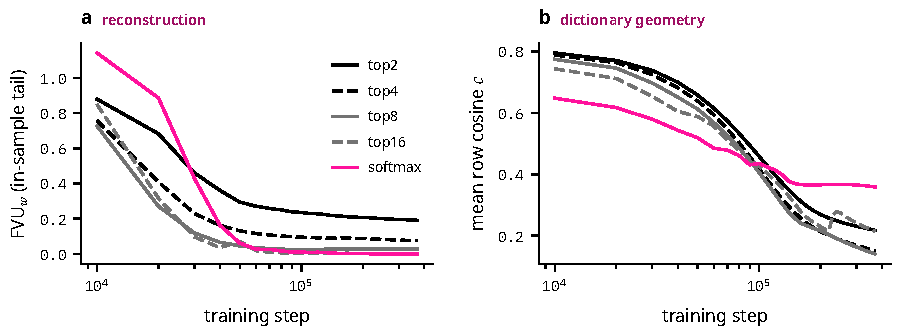
\includegraphics[width=\linewidth]{figures/fig-sweep-curves.pdf}
\caption{Training trajectories of the \texttt{\_shm} arms in the SONAR
selection sweep: (a) $\fvu$ on the (in-sample) evaluation tail, scored from
each checkpoint, and (b) mean within-head atom cosine $\bar\kappa$. The
soft arm's $\bar\kappa$ flattens near $0.36$ while its error continues to
fall, whereas the harder arms continue decorrelating their atoms.}
\label{fig:sweep-curves}
\end{figure}

\paragraph{Inertness of the final layer at low residual error.} Whereas
within-head atom collinearity decreases monotonically with depth in every
hard arm, it spikes in the final layer of the soft arms (reaching
$\bar\kappa{=}0.799$ and effective rank $1.54$ in layer 4 of
\texttt{softmax\_shm}). To separate collinearity from exhausted residual
variance, \texttt{lastlayer.py} ablates the final layer's heads in two
ways---uniform ablation (emitting each head's mean atom) and zero ablation
(emitting zero):

\begin{center}\small
\begin{tabular}{@{}llrrrrr@{}}
\toprule
arm & select & L4 $\bar\kappa$ & L4 eff & \stackhead[r]{prefix $\fvu$\\before L4} & L4 adds & zero-ablate \\
\midrule
top1         & top1    & $+0.246$ & 10.60 & 0.7511 & $+4.3\%$  & $+4.5\%$ worse \\
top2\_shm    & top2    & $+0.188$ & 14.89 & 0.2378 & $+19.7\%$ & $+24.5\%$ worse \\
top8\_shm    & top8    & ---      & ---   & 0.0304 & $+5.5\%$  & $+5.8\%$ worse \\
top16\_shm   & top16   & $+0.433$ & 3.46  & 0.0043 & $+0.0\%$  & $+0.0\%$ \\
softmax      & softmax & $+0.263$ & 6.00  & 0.0023 & $-1.2\%$  & $-1.1\%$ better \\
softmax\_shm & softmax & $+0.799$ & 1.54  & 0.0007 & $-1.9\%$  & $-1.8\%$ better \\
\bottomrule
\end{tabular}
\end{center}

Whether the final layer helps depends on the residual error entering it
rather than on its atom collinearity: layer 4 of \texttt{softmax} is not
collapsed ($\bar\kappa{=}0.263$) yet is equally unhelpful. Once prefix
$\fvu$ before layer 4 falls below roughly $0.005$, the final layer becomes
inert or slightly harmful, which accounts for the mildly harmful layer 4 of
\texttt{resid\_nc} (prefix $\fvu = 0.0051$) without invoking its frozen
heads. Nevertheless, the two low-error regimes end differently: in
\texttt{top16\_shm}, layer 4 shrinks its atom norms to 4\% of those in
earlier layers and emits virtually nothing, whereas in
\texttt{softmax\_shm}, layer 4 retains comparable atom magnitudes that
become highly collinear, emitting a nearly constant vector whose removal
slightly reduces reconstruction error (reflecting mild overfitting rather
than a useful bias).

\paragraph{Comparison against an unpartitioned kernel smoother.} The
leave-one-out noise2self partition score corresponding to
$\mathrm{L2}_{\mathrm{pwak}}$ can be evaluated post hoc on the selection
sweep (Figure~\ref{fig:selection}, \texttt{selection.py}), measuring how
accurately a sample's co-classified neighbors predict its layer input
relative to the same heat-kernel smoother with all samples placed in a
single cell (none of the sweep arms trained with
$\mathrm{L2}_{\mathrm{pwak}}$ active). Across all arms, gating by a head's
partition improves over that smoother by at most $0.020$ in layer 0
(\texttt{top4\_shm}), by at most $0.005$ in layers 1--3, and by $0.031$ in
layer 4 only for \texttt{softmax} (where layer 4 is already inert). A
random partition with matched cell sizes never improves over the smoother,
and a single-entry code (\texttt{top1}) performs worse than the smoother
above layer 0. Because this leave-one-out score is not
$\mathcal{J}$-invariant (Appendix~\ref{app:methods}), the row-permuted
partition serves as a floor only for partitions that do not depend on the
input: any partition computed from the input---whether trained or
not---can improve on the smoother without clustering genuine modes. Each
arm uses one seed and was trained on the evaluation tail.

\paragraph{$\mathcal{J}$-invariant evaluation and random-projection baselines.}
Evaluating the coordinate-split $\mathcal{J}$-invariant estimator
(Appendix~\ref{app:methods}) across all 76 heads per layer of
\texttt{ste\_h76\_init01} resolves both the bandwidth and self-leakage
confounds (\texttt{selection.py --jinv}; one seed). Bandwidth selection
under the split estimator chooses $0.05$ in layers 0 and 4 and $0.03$ in
layers 1--3; in layer 0, narrowing the unpartitioned smoother's bandwidth
from Figure~\ref{fig:selection}'s $0.2$ to $0.05$ lowers its error by
$0.112$, exceeding the largest gain achieved by any single head or
multi-head gate at bandwidth $0.2$ (at most $0.060$). Furthermore, a
random-projection head acts as an angular locality-sensitive
hash~\cite{harpeled2012}: because the probability that it places two rows
in the same cell decreases as the angle between them grows, gating a wide
heat kernel by random projections sharpens the kernel much like reducing
its bandwidth. At bandwidth $0.2$, a single random-projection head improves
over the smoother by $0.017$ under the leave-one-out score but by $-0.001$
(no gain) under the split estimator, showing that its single-head gain came
from self-leakage, whereas the joint gate of eight random heads and the
random collision kernel retain gains of $0.042$ and $0.047$ because they
sharpen an over-wide kernel. At the selected bandwidth, single trained
heads score worse than the unpartitioned smoother in every layer (by
$0.040$ in layer 0, $0.065$--$0.069$ in layers 1--3, and $0.030$ in
layer 4), matching single random-projection heads ($0.030$ and
$0.063$--$0.068$). Likewise, the joint gate across a layer's trained heads
improves over the smoother by $0.034$ in layer 0 and $0.005$--$0.006$ in
layers 1--4, closely tracked by the random-projection collision kernel
($0.039$ and $0.005$--$0.009$). Because trained heads depend on all input
coordinates, comparisons involving trained heads use the leave-one-out
estimator; relative to random-projection heads, learned partitions exhibit
no structure beyond angular locality. On isotropic inputs, the
coordinate-split estimator maintains its null floor down to a bandwidth of
$0.05$, whereas the leave-one-out estimator drops below the floor by
$0.010$ at bandwidth $0.2$ and by $0.090$ at bandwidth $0.02$, quantifying
its self-prediction leak.

\begin{figure}[tp]
\centering
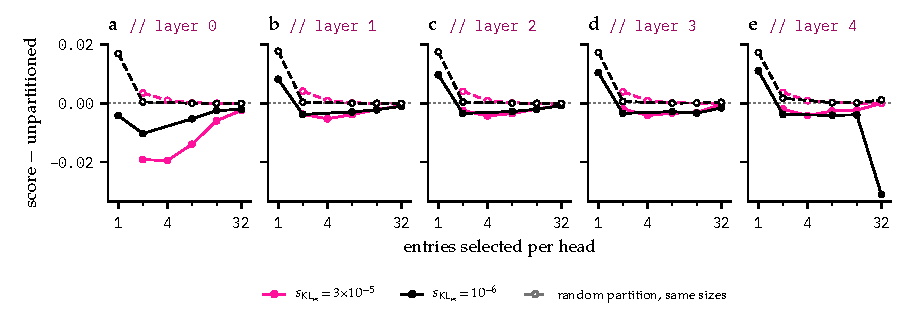
\includegraphics[width=\linewidth]{figures/fig-selection.pdf}
\caption[Held-out noise2self score against the selection
rule]{\textbf{Learned partitions barely improve over an unpartitioned
	smoother.} Leave-one-out noise2self score per layer across the SONAR
	selection sweep as a function of the number of selected entries per head
	($1$ for argmax, $32$ for softmax), shown relative to the same run's
	score when all rows are placed in a single cell (values below $0$
	indicate an improvement from partitioning), both with and without the
	batch-mean uniformity term $\mathrm{KL}_m$. Filled markers show mean
	scores across learned head partitions; hollow markers with dashed lines
	show row-permuted assignments (random partitions with matched cell
	sizes). Evaluated with a bandwidth-$0.2$ heat kernel on each layer's
	input in batches of 2{,}048 rows; one seed per arm on the in-sample
	tail.}
\label{fig:selection}
\end{figure}

\subsection{Bilinear classifier geometry from model weights}
\label{sec:bilinspec}

Each classifier logit is computed by a single bilinear factor pair
$(\mathbf{w}\cdot\mathbf{u})(\mathbf{v}\cdot\mathbf{u})$, so the factor
alignment $\lvert\cos\angle(\mathbf{w},\mathbf{v})\rvert$ characterizes the
quadratic form directly. When $\lvert\cos\angle(\mathbf{w},\mathbf{v})\rvert$
is near $1$, the form approaches rank 1 and is proportional to
$(\mathbf{w}\cdot\mathbf{u})^2$, which is even in $\mathbf{u}$ and
therefore invariant to flipping the input's sign along $\mathbf{w}$. When
$\lvert\cos\angle(\mathbf{w},\mathbf{v})\rvert$ is near $0$, the form
defines an indefinite saddle that distinguishes whether its two projections
share the same sign, yet remains equally even on the semantic coordinates
because $(\mathbf{w}\cdot(-\mathbf{u}))(\mathbf{v}\cdot(-\mathbf{u})) =
(\mathbf{w}\cdot\mathbf{u})(\mathbf{v}\cdot\mathbf{u})$. Thus, rank
changes the shape of the region to which a feature responds rather than its
sign symmetry, which only the appended constant coordinate can break (see
Appendix~\ref{app:methods} for protocol details).
Figure~\ref{fig:bilinspec} evaluates this alignment directly from the
weights of the softmax stack (\texttt{resid\_nc}) and the hard-code stack
(\texttt{ste\_h76\_init01}).

The softmax stack's classifiers converge toward rank-1 forms in
intermediate layers, whereas the hard-code stack's classifiers mostly do
not. At the final checkpoint, median $\lvert\cos\angle\rvert$ in the
softmax stack reaches $0.94$ in layer 1 and $0.52$--$0.80$ in layers 2--3,
whereas layers 1--3 of the hard-code stack remain at $0.10$--$0.16$
(compared to $0.021$ for random vector pairs). Layer 0 reaches
$0.54$--$0.64$ in both models, while layer 4 of the softmax stack falls to
$0.18$. Factor alignment develops relatively late in training: every layer
starts at the random floor, with the softmax stack departing between 30k
and 50k steps as temperature annealing finishes, and the hard-code stack
departing only after 80k steps in layer 0 and 220k steps in layers 3--4
(with layers 1--2 exceeding $0.05$ only at the final checkpoint). The
dominant eigenvalue is negative for 63--98\% of features in the softmax
stack and 97--99\% in the hard-code stack, meaning that a rank-1 feature
takes its largest values where the input is orthogonal to $\mathbf{w}$
rather than aligned with it---implementing the quadratic invariances that
bilinear layers learn in place of constants~\cite{pearce2025}. Finally, the
constant coordinate can break the sign symmetry of a rank-1 feature for
inputs weakly aligned with $\mathbf{w}$: across layers 1--4, its weight
magnitude equals $0.18$--$0.24$ of the norm of the remaining coordinates of
$\mathbf{w}$ in the softmax stack, compared to $0.017$--$0.025$ in the
hard-code stack. This analysis uses one seed per run and inspects model
weights only.

\begin{figure}[tp]
\centering
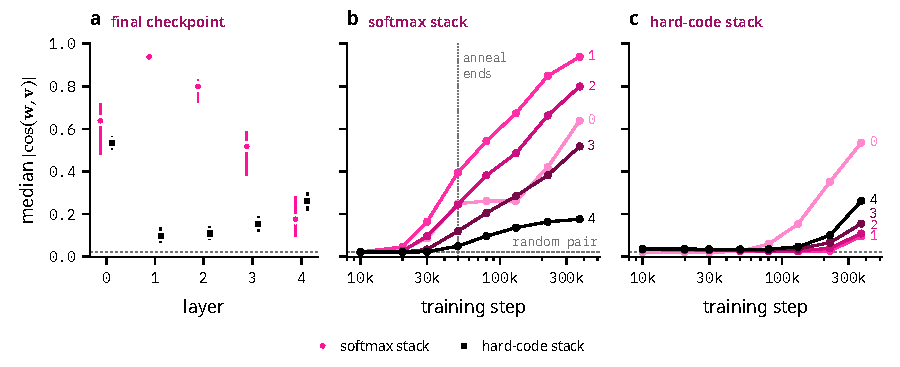
\includegraphics[width=\linewidth]{figures/fig-bilinspec.pdf}
\caption[Classifier geometry from the weights]{\textbf{Bilinear classifiers
	approach rank 1 in the softmax stack but remain mostly rank 2 in the
	hard-code stack.} Median factor alignment
	$\lvert\cos\angle(\mathbf{w},\mathbf{v})\rvert$ across bilinear feature
	pairs per layer (\texttt{bilinspec.py}; $1$ indicates a rank-1 feature).
	(a) Final-checkpoint medians and interquartile ranges by layer for the
	softmax stack (\texttt{resid\_nc}, step 372.6k) and the hard-code stack
	(\texttt{ste\_h76\_init01}, step 369.5k). (b, c) Evolution over training,
	with one curve per layer labeled at its right endpoint; temperature
	annealing in the softmax stack ends at step 50k, whereas the hard-code
	stack uses a constant temperature. Dashed lines mark the median for a
	random pair in the 1024-dimensional semantic block ($0.021$). One seed
	per run.}
\label{fig:bilinspec}
\end{figure}
